% Organizing document for the Infernal User's Guide
%
% SVN $Id$


\documentclass[10pt]{article}
%\usepackage{helvetic}
\usepackage{times}
\usepackage{fullpage}
\usepackage{fancybox}  % Must include fancybox *before* fancyvrb;
\usepackage{fancyvrb}  % don't know why.
\usepackage[pdftex]{graphicx}
\usepackage{url}
%\usepackage[backref,colorlinks]{hyperref}
\usepackage[authoryear]{natbib}

\usepackage{verbatim}

\setcounter{secnumdepth}{1}
\renewcommand{\familydefault}{\sfdefault}
% customizations used in the User's Guide


% Description-like environment for documenting functions/APIs.
% puts the description label in a minipage with a large hanging
% indent.
% Good christ this took a long time to develop.
% hanging indent trick stolen from Peter Wilson's hanging.sty @CTAN
% minipage allows multi-line label, and puts item on next line.
% customized list inspired by Kopka/Daly _Guide to LaTeX_ p.213
% SRE, Wed Dec 27 11:37:18 2000
%
\newenvironment{sreapi}{%
     \begin{list}{}{%
       \renewcommand{\makelabel}[1]{%
         \begin{minipage}{\textwidth}%
           \hangindent10em\hangafter1\noindent%
           {\bfseries\texttt{##1}\vspace{0.8em}}%
         \end{minipage}%
     }}}%
     {\end{list}}


% Description-like environment for producing lists like:
%
%     label  stuff, stuff, stuff
%
%    label2  more stuff, more stuff,
%            more stuff.
% \begin{sreitems}{Longest label} \item[label] stuff, ... \end{sreitems}
% SRE, Wed Dec 27 11:59:43 2000
%
\newenvironment{sreitems}[1]{%
     \begin{list}{}{%
       \settowidth{\labelwidth}{#1}%
       \setlength{\leftmargin}{\labelwidth}%
       \addtolength{\leftmargin}{\labelsep}%
       }}
     {\end{list}}
       
\DefineVerbatimEnvironment{sreoutput}{Verbatim}{fontsize=\scriptsize,xleftmargin=2.0\parindent}%
\DefineVerbatimEnvironment{tinysreoutput}{Verbatim}{fontsize=\tiny,xleftmargin=2.0\parindent}%

\makeatletter
\newcommand{\listoffaqs}{\@starttoc{faq}}
\newenvironment{srefaq}[1]
{\addcontentsline{faq}{faq}{#1}\begin{sloppypar}\noindent\slshape\small\begin{quote}\textbf{$\triangleright$ #1}}
{\end{quote}\end{sloppypar}}
\newcommand{\l@faq}[2]{\@dottedtocline{0}{0pt}{0pt}{#1}{#2}}
\makeatother


% Consistent font styles
%   \software{}   for the name of a software package
%   \database{}   for the name of a database
%   \prog{}       for a program or file name
%   \emprog{}     for an emphasized program or file name
%   \user{}       for a typed user command
%   \scriptuser{} scriptsize typed user command
%   \response{}   for an output line following a \user command
%   \ccode{}      for an inlined C code phrase
\newcommand{\software}[1]{\textsc{#1}}
\newcommand{\database}[1]{\textsc{#1}}
\newcommand{\prog}[1]{{\small\bfseries\texttt{#1}}}
\newcommand{\emprog}[1]{{\small\bfseries\texttt{#1}}}
\newcommand{\user}[1]{\indent\indent{\small\bfseries\texttt{> #1}}}
\newcommand{\scriptuser}[1]{\indent\indent{\scriptsize\bfseries\texttt{> #1}}}
\newcommand{\response}[1]{\indent\indent{\small\bfseries\texttt{#1}}}
\newcommand{\ccode}[1]{{\small\texttt{#1}}}

\DefineVerbatimEnvironment{cchunk}{Verbatim}{fontsize=\scriptsize,xleftmargin=2.0\parindent}%

% The ``wideitem'' environment is mostly obsolete, but
% it gets used in converted manpages.
%
\newenvironment{wideitem}{\begin{list} 
     {}
     { \setlength{\labelwidth}{2in}\setlength{\leftmargin}{1.5in}}}
     {\end{list}}


% The following are used as temp vars in how man pages are 
% converted into LaTeX w/ rman; see ``make manpages'' in Makefile.
\newlength{\sresavei}
\newlength{\sresaves}

\def\argmax{\mathop{\mathrm{argmax}}\limits}
\def\argmin{\mathop{\mathrm{argmin}}\limits}

% The sidebar environment, for inserting ``asides''.
% Requires the ``fancybox'' package.
% Example:
%   \usepackage{fancybox}
%   ...
%   \begin{sidebar}
%   \sidebarhead{An aside on string theory.}
%   String theory is not mentioned in this document.
%   \end{sidebar}
%
% SRE, Sun Nov  6 14:45:32 2005
%
\newenvironment{sidebar}%
  {\begin{Sbox}\begin{minipage}{\textwidth}\setlength{\parskip}{0.5em}}%
  {\end{minipage}\end{Sbox}%
   \begin{figure}[htp]\shadowbox{\TheSbox}\end{figure}%
   \setlength{\parskip}{0em}}
\newcommand{\sidebarhead}[1]{{\bfseries{#1}}\vspace{0.3em}}


\begin{document}

\bibliographystyle{apalike}

\begin{titlepage}
{\Large

\vspace*{\fill}

\begin{latexonly}
\noindent
{\Huge \textsf{INFERNAL User's Guide}} \\ 
\rule[2pt]{\textwidth}{1pt} \\
\hspace*{\fill} {\large \textsf{Sequence analysis using profiles of RNA secondary structure consensus}\\}
\end{latexonly}

\begin{htmlonly}
\begin{center}
{\Huge \textbf{INFERNAL User's Guide}}\\
{\large \textbf{Sequence analysis using profiles of RNA secondary
structure consensus}}\\
\end{center}
\end{htmlonly}

\vspace*{\fill}

\begin{center}
\textsl{\htmladdnormallink{http://infernal.wustl.edu/}{http://infernal.wustl.edu/}}\\
Versions 0.x; March 2003 \\ 

\vspace*{\fill}

Sean Eddy\\
Howard Hughes Medical Institute and Dept. of Genetics\\
Washington University School of Medicine\\
660 South Euclid Avenue, Box 8232\\
Saint Louis, Missouri 63110, USA\\
\textsl{eddy@genetics.wustl.edu} \\
\end{center}

\vspace*{\fill}

}
\end{titlepage}

\vspace*{\fill}
\begin{flushleft}
Copyright (C) 2012 Howard Hughes Medical Institute.\vspace{5mm}

\vspace{5mm}
Permission is granted to make and distribute verbatim copies of this
manual provided the copyright notice and this permission notice are
retained on all copies.\vspace{5mm}

\vspace{5mm} INFERNAL is licensed and freely distributed under the GNU
General Public License version 3 (GPLv3). For a copy of the License,
see \url{http://www.gnu.org/licenses/}.

\vspace{5mm}
\end{flushleft}




\newpage
\tableofcontents

\newpage
\section{Introduction}
\label{section:introduction}
\setcounter{footnote}{0}

Infernal is used to search sequence databases for homologs of
structural RNA sequences, and to make sequence- and structure-based
RNA sequence alignments. Infernal builds a \emph{profile} from a
structurally annotated multiple sequence alignment of an RNA family
with a position-specific scoring system for substitutions, insertions,
and deletions. Positions in the profile that are basepaired in the
  h consensus secondary structure of the alignment are modeled as
dependent on one another, allowing Infernal's scoring system to
consider the secondary structure, in addition to the primary sequence,
of the family being modeled. Infernal profiles are probabilistic
models called ``covariance models'', a specialized type of stochastic
context-free grammar (SCFG) \citep{Lari90}.

Compared to other alignment and database search tools based only on
sequence comparison, Infernal aims to be significantly more accurate
and more able to detect remote homologs because it models sequence
and structure. But modeling structure comes at a high computational
cost, and the slow speed of CM homology searches has been a serious
limitation of previous versions. With
version 1.1, typical homology searches are now about 100x faster,
thanks to the incorporation of accelerated HMM methods from the HMMER3
software package (\url{http://hmmer.org}), making Infernal a much more
practical tool for RNA sequence analysis.

\subsection{How to avoid reading this manual}

If you're like most people, you don't enjoy reading documentation.
You're probably thinking: \pageref{manualend} pages of documentation,
you must be joking! I just want to know that the software compiles,
runs, and gives apparently useful results, before I read some
\pageref{manualend} exhausting pages of someone's documentation. For
cynics that have seen one too many software packages that don't work:

\begin{itemize}
\item Follow the quick installation instructions on page
      \pageref{section:installation}. An automated test suite
      is included, so you will know immediately if something
      went wrong.\footnote{Nothing should go wrong.}
\item Go to the tutorial section on page
\pageref{section:tutorial}, which walks you through some examples of
using Infernal on real data.
\end{itemize}

Everything else, you can come back and read later.

\subsection{What covariance models are}

Covariance models (CMs) are statistical models of structurally
annotated RNA multiple sequence alignments, or even of single
sequences and structures. CMs are a specific formulation of profile
stochastic context-free grammars (profile SCFG), which were introduced
independently by Yasu Sakakibara in David Haussler's
group \citep{Sakakibara94c} and by Sean Eddy and Richard
Durbin \citep{Eddy94}. CMs are closely related to profile hidden Markov
models (profile HMMs) commonly used for protein sequence analysis, but
are more complex. CMs and profile HMMs both capture position-specific
information about how conserved each column of the alignment is, and
which residues are likely. However, in a profile HMM each position of
the profile is treated independently, while in a CM basepaired
positions are dependent on one another.  The dependency between paired
positions in a CM enables the profile to model \emph{covariation} at
these positions, which often occurs between basepaired columns of
structural RNA alignments. For many of these basepairs, it is not the
specific nucleotides that make up the pair that is conserved by
evolution, but rather that the pair maintain Watson-Crick
basepairing. The added signal from covariation can be significant when
using CMs for homology searches in large
databases. Section~\ref{section:cmbuild} of this guide explains how a
CM is constructed from a structurally annotated alignment using a toy
example. 

CMs do have important limitations though. For example, a CM can only
model what is called a ``well-nested'' set of basepairs. Formally, in
a well-nested set of basepairs there are no two basepairs between
positions $i:j$ and $k:l$ such that $i<k<j<l$. CMs cannot model
pseudoknots in RNA secondary structures. Additionally, a CM only
models a single consensus structure for the family it models. 

\subsection{Applications of covariance models}

Infernal can be useful if you're intereseted in a particular RNA
family. Imagine that you've carefully collected and aligned a set of
homologs and have a predicted (or known) secondary structure for the
family. Homology searches with BLAST using single sequences from your
set of homologs may not reveal any additional homologs in sequence
databases. You can build a CM from your alignment and redo your search
using Infernal (this time only a single search) and you may find new
homologs thanks to the added power of the profile-based sequence and
structure scoring system of CMs. The Rfam database \citep{Gardner11}
essentially does just this, but on a much larger scale. The Rfam
curators maintain about 2000 RNA families, each represented by a
multiple sequence alignment (called a \emph{seed} alignment) and a CM
built from that alignment. Each Rfam release involves a search through
a large EMBL-based nucleotide sequence database with each of the CMs
which identifies putative structural RNAs in the database. The
annotations of these RNAs, as well as the CMs and seed alignments are
freely available.

Automated genome annotation of structural RNAs can be performed with
Infernal and a collection of CMs from Rfam, by searching
through the genome of interest with each CM and collecting information
on high-scoring hits. Previous versions of Infernal were too slow to
be incorporated into many genome annotation pipelines, but we're
hoping the improved speed of version 1.1 changes this.

Another application is the automated construction and maintenance of
large sequence- and structure-based multiple alignment databases.  For
example, the Ribosomal Database Project uses CMs of 16S small subunit
ribosomal RNA (16S SSU rRNA) to maintain alignments of millions of 16S
sequences \citep{Cole09}. The CMs (one archaeal 16S and one bacterial
16S model) were built from training alignments of only a few hundred
representative sequences. The manageable size of the training
alignments means that they can be manually curated prior to building
the model. Rfam is another example of this application too because
Rfam creates and makes available multiple alignments (called \emph{full}
alignments) of all of the hits from the database its curators believe
to be real RNA homologs.

Infernal can also be used to determine what types of RNAs exist in a
particular sequence dataset. Suppose you're performing a metagenomics
analysis and have collected sequences from an exotic environmental
sample. You can download all the CMs from Rfam and use Infernal to
search through all your sequences for high-scoring hits to the
models. The types of structural RNAs identified in your sample can be
informative as to what types of organisms are in your sample, and what
types of biological processes they're carrying out. Version 1.1
includes a new program called \prog{cmscan} which is designed for just
this type of analysis.

\subsection{Infernal and HMMER, CMs and profile HMMs}

Infernal is closely related to HMMER. In fact, HMMER is used as a
library within the Infernal codebase. This allows Infernal to use the
highly optimized profile HMM dynamic programming implementations in
HMMER to greatly accelerate its homology searches. Also, the design
and organization of the Infernal programs (e.g. \ccode{cmbuild},
\ccode{cmsearch}, \ccode{cmalign}) follows that in HMMER
(\ccode{hmmbuild}, \ccode{hmmsearch}, \ccode{hmmalign}). And there are
many functions in Infernal that are based on analogous ones in
HMMER. The formatting of output is often very similar between
these two software packages, and the user guide's are even organized
and written in a similar (and, in some places, identical) way. 

This is, of course, on purpose. Since both packages are developed in
the same lab, consistency simplifies the development and maintenance
of the code, but we also do it to make the software (hopefully) easier
to use (someone familiar with using HMMER should be able to pick up
and use Infernal very easily, and vice versa). However, Infernal
development tends to lag behind HMMER development as new ideas and
algorithms are applied to the protein or DNA world with profile HMMs,
and then later extended to CMs for use on RNAs.
%Some of the current features of HMMER are on
%the 00TODO list for Infernal (and by the time they're implemented they
%will have been replaced on that list).

This consistency is possible because profile HMMs and covariance
models are related models with related applications.  Profile HMMs are
profiles of the conserved sequence of a protein or DNA family and CMs
are profiles of the conserved sequence \emph{and} well-nested
secondary structure of a structural RNA family. Applications of
profile HMMs include annotating protein sequences in proteomes or
protein sequence database and creating multiple alignments of protein
domain families. And similarly applications of CMs include annotating
structural RNAs in genomes or nucleotide sequence databases and
creating sequence- and structure-based multiple alignments of RNA.
The crucial difference is that CMs are able to model dependencies
between a set of well-nested (non-pseudoknotted) basepaired positions
in a structural RNA family. The statistical signal inherent in these
dependencies is often significant enough to make modeling the family
with a CM a noticeably more powerful approach than modeling the family
with a profile HMM.

\subsection{Differences between Infernal 1.1x and earlier versions}

The most important difference between version 1.1 and the previous
version (1.0.2) is the improved search speed that results from a new
filter pipeline. The pipeline is explained more in
section~\ref{section:pipeline}. Another important change is the
introduction of the \prog{cmscan} program, for users who want to know
what structural RNAs are present in a collection of sequences, such as
a metagenomics dataset\footnote{\prog{cmscan} is similar to
\prog{cmsearch} but is more convenient for some applications. One
difference between the two programs is that results from \prog{cmscan}
are organized per-sequence instead of per-model.}. Another new feature
of version 1.1 is better handling of truncated RNAs, for which part of
one or both ends of the RNA is missing due to a premature end of the
sequence \citep{KolbeEddy09}. These types of fragmentary sequences are
common in whole genome shotgun sequencing datasets. While previous
versions of Infernal were prone to misalignment of these sequences,
version 1.1 includes implementations of CM search and alignment
algorithms specialized for truncated sequences \citep{KolbeEddy09} in
\prog{cmsearch}, \prog{cmscan} and \prog{cmalign}.

Model parameterization has changed in several minor ways. Mixture
Dirichlet priors for emissions and single component Dirichlet priors
for transitions have been reestimated using larger and more diverse
datasets than the ones the previous priors were derived from
(discussed in \citep{NawrockiEddy07}). Also, the definition of match
and insert columns, previously determined by a simple majority rule
using absolute counts (columns in which $\geq 50\%$ of columns include
residues were match, all others were insert), now use \emph{weighted}
counts (and same $>=50\%$ rule) after a sequence weighting algorithm
is applied. And inserts before the first and after the final match
position of alignments are now ignored by the CM construction
procedure and thus no longer contribute to parameterizing the
transition probabilities of the model (specifically, the
\ccode{ROOT\_IL} and \ccode{ROOT\_IR} states). These changes mean
that for a given input alignment a model built with version 1.1 may
have different numbers of states and nodes, and will have (usually)
slightly different parameters, than a model built from the same
alignment with version 1.0.2.  Finally, the important \prog{cmbuild}
command line options \prog{--rf} and \prog{--gapthresh} have been
renamed to \prog{--hand} and \prog{--symfrac}\footnote{To reproduce
the behavior obtained in previous versions with \prog{--gapthresh <x>}
use \prog{--symfrac <1-x>}.}.

The formatting of \prog{cmsearch} output has also changed. It mirrors
the output format of the \prog{hmmsearch} program from HMMER3, for
examples see the tutorial section of this guide. Another change is
that the most compute-intensive programs in Infernal 1.1
(\prog{cmcalibrate}, \prog{cmsearch}, \prog{cmscan} and
\prog{cmalign}) support multicore parallelization using threads.

\subsection{How to learn more about CMs and profile HMMs}

Section~\ref{section:cmbuild} of this guide may be a good place to
start. That section walks through an example of how a CM is
constructed from a structurally annotated multiple sequence alignment.
The tutorial section is also recommended for all users.

As for other available publications: two papers published in 1994
introduced profile SCFGs in computational biology
\citep{Sakakibara94c,Eddy94}, and our lab has published several papers
\citep{Eddy02b,KleinEddy03,NawrockiEddy07,Nawrocki09,KolbeEddy09,KolbeEddy11},
book chapters \citep{Eddy06b,Nawrocki14}, and a few doctoral
theses \citep{Klein03,Nawrocki09b,Kolbe10} related to
CMs\footnote{Eddy lab publications are available from
\url{http://eddylab.org/publications.html}}. The book
\emph{Biological Sequence Analysis: Probabilistic Models of Proteins
and Nucleic Acids} \citep{Durbin98} has several chapters devoted to
HMMs and CMs. Profile HMM filtering for CMs was introduced by Weinberg
and Ruzzo
\citep{WeinbergRuzzo04,WeinbergRuzzo04b,WeinbergRuzzo06}. There are
two papers from our lab on HMMER3 profile HMMs that are directly
related to Infernal's accelerated filter pipeline
\citep{Eddy08,Eddy11}.

Since CMs are closely related to, but more complex than, profile HMMs,
readers seeking to understand CMs who are unfamiliar with profile HMMs
may want to start there.  Reviews of the profile HMM literature have
been written by our lab \citep{Eddy96,Eddy98} and by Anders Krogh
\citep{Krogh98}. And to learn more about HMMs from the perspective of
the speech recognition community, an excellent tutorial introduction
has been written by Rabiner \citep{Rabiner89}. For details on how
profile HMMs and probabilistic models are used in computational
biology, see the pioneering 1994 paper from Krogh et
al. \citep{Krogh94} and again the \emph{Biological Sequence Analysis}
book \citep{Durbin98}.

Finally, Sean Eddy writes about HMMER, Infernal and other lab projects in
his blog \textbf{Cryptogenomicon} \url{http://cryptogenomicon.org/}).

\subsection{How do I cite Infernal?}

If you'd like to cite a paper, please cite the Infernal 1.1 application
note in \emph{Bioinformatics}:

Infernal 1.1: 100-fold faster RNA homology searches.
EP Nawrocki and SR Eddy.
Bioinformatics, 29:2933-2935, 2013.

The most appropriate citation is to the web site,
\url{http://eddylab.org/infernal/}. You should also cite what version
of the software you used. We archive all old versions, so anyone
should be able to obtain the version you used, when exact
reproducibility of an analysis is an issue.

The version number is in the header of most output files. To see it
quickly, do something like \prog{cmscan -h} to get a help page, and
the header will say:

\begin{sreoutput}
# cmscan :: search sequence(s) against a CM database
# INFERNAL 1.1.5 (Sep 2023)
# Copyright (C) 2023 Howard Hughes Medical Institute.
# Freely distributed under the BSD open source license.
# - - - - - - - - - - - - - - - - - - - - - - - - - - - - - - - - - - - -
\end{sreoutput}

So (from the second line there) this is from Infernal 1.1.5.

\subsection{How do I report a bug?}

Open an issue on our issue tracker at GitHub\footnote{GitHub issue
  tracker: \url{https://github.com/EddyRivasLab/infernal/issues}} or email us,
at \url{eric.nawrocki@nih.gov}.

Before we can see what needs fixing, we almost always need to
reproduce a bug on one of our machines. This means we want to have a
small, reproducible test case that shows us the failure you're seeing.
So if you're reporting a bug, please send us:

\begin{itemize}
 \item A brief description of what went wrong.
 \item The command line(s) that reproduce the problem.
 \item Copies of any files we need to run those command lines.
 \item Information about what kind of hardware you're on, what
   operating system, and (if you compiled the software yourself rather
   than running precompiled binaries), what compiler and version you
   used, with what configuration arguments.
\end{itemize}

Depending on how glaring the bug is, we may not need all this
information, but any work you can put into giving us a clean
reproducible test case doesn't hurt and often helps.

The information about hardware, operating system, and compiler is
important. Bugs are frequently specific to particular configurations
of hardware/OS/compiler.  We have a wide variety of systems available
for trying to reproduce bugs, and we'll try to match your system as
closely as we can.

If you first see a problem on some huge compute (like running a
zillion query sequence over a huge profile database), it will really,
really help us if you spend a bit of time yourself trying to isolate
whether the problem really only manifests itself on that huge compute,
or if you can isolate a smaller test case for us. The ideal bug report
(for us) gives us everything we need to reproduce your problem in one
email with at most some small attachments. 

Remember, we're not a company with dedicated support staff -- we're a
small lab of busy researchers like you. Somebody here is going to drop
what they're doing to try to help you out. Try to save us some time,
and we're more likely to stay in our usual good mood.

If we're in our usual good mood, we'll reply quickly.  We'll probably
tell you we fixed the bug in our development code, and that the fix
will appear in the next Infernal release. This of course doesn't help you
much, since nobody knows when the next Infernal release is going to be.
So if possible, we'll usually try to describe a workaround for the
bug.

If the code fix is small, we might also tell you how to patch and
recompile the code yourself. You may or may not want to do this.













  











\newpage
\section{Installation}

\subsection{Quick installation instructions from source}

Download the source tarball (\prog{infernal.tar.gz}) from 
\htmladdnormallink{ftp.genetics.wustl.edu/pub/eddy/software/infernal/}
                  {ftp://ftp.genetics.wustl.edu/pub/eddy/software/infernal/}
or 
\htmladdnormallink{www.genetics.wustl.edu/eddy/infernal/}
                  {http://www.genetics.wustl.edu/eddy/infernal/}.


Unpack, configure, make, and test the software:
  
\begin{center}\begin{minipage}{5.5in}
\user{tar xvf infernal.tar.gz}
\user{cd infernal}
\user{./configure}
\user{make}
\user{make check}
\end{minipage}\end{center}

All the tests should pass.

The programs are in the \prog{src/} subdirectory. The user's guide
(this document) is in the \prog{documentation/userguide}
subdirectory. The man pages are in the \prog{documentation/manpages}
subdirectory. You can manually move or copy all of these to
appropriate locations if you want. You will want the programs to be in
your \$PATH.

More complete instructions follow, including how to install the
package automatically with \prog{make install}.

\subsection{Detailed installation notes}

\subsection{Supported platforms}

\subsection{Configuration options}

\package{Infernal} uses a GNU configure script to automatically
configure the source code for your platform. Normally 

\begin{sreitems}
\item[--enable-lfs] 
\item[




\newpage
% EPN, Mon Oct 21 12:57:38 2013
% Actual commands run on: 
% login-eddy

\section{Tutorial}
\label{section:tutorial}
\setcounter{footnote}{0}

Here's a tutorial walk-through of some small projects with
Infernal. This should suffice to get you started on work of your own,
and you can (at least temporarily) skip the rest of the Guide,
such as all the nitty-gritty details of available command line
options.

\subsection {The programs in Infernal}


\begin{tabular}{ll}
\multicolumn{2}{c}{\textbf{Core programs}}\\
 & \\ 
\textbf{cmbuild}     & Build a covariance model from an input multiple alignment.\\
\textbf{cmcalibrate} & Calibrate E-value parameters for a covariance model.\\
\textbf{cmsearch}    & Search a covariance model against a sequence database.\\
\textbf{cmscan}      & Search a sequence against a covariance model database.\\
\textbf{cmalign}     & Make a multiple alignment of many sequences to a common covariance model.\\
 & \\ 
\multicolumn{2}{c}{\textbf{Other utilities}}\\ 
 & \\ 
\textbf{cmconvert} & Convert CM formats to/from Infernal v1.1 format.\\ 
\textbf{cmemit}    & Generate (sample) sequences from a covariance model.\\
\textbf{cmfetch}   & Get a covariance model by name or accession from a CM database.\\
\textbf{cmpress}   & Format a CM database into a binary format for \prog{cmscan}.\\
\textbf{cmstat}    & Show summary statistics for each model in a CM database.\\ 
\end{tabular} \\
\\

In this section, we'll show examples of running each of these
programs, using examples in the \otext{tutorial/} subdirectory of the
distribution.

\subsection{Files used in the tutorial}

The subdirectory \otext{/tutorial} in the Infernal distribution contains the
files used in the tutorial, as well as a number of examples of various
file formats that Infernal reads. The important files for the tutorial
are:

\begin{sreitems}{\emprog{minifam.i1\{m,i,f,p\}}}
\item[\otext{tRNA5.sto}] A multiple alignment of five tRNA
  sequences. This file is a simple example of \emph{Stockholm
  format} that Infernal uses for structurally-annotated alignments.
%
\item[\otext{tRNA5.c.cm}] An example CM file. Built with
  \prog{cmbuild} from \otext{tRNA5.sto} and calibrated using
  \prog{cmcalibrate}. Included so you don't need to calibrate your own
  model file, which takes about 20 minutes. 
%
\item[\otext{mrum-genome.fa}] The 3 Mb genome of the methanogenic archeaon 
  \emph{Methanobrevibacter ruminantium}, in
  FASTA format, downloaded from the NCBI Nucleotide database
  (accession: NC\_13790.1). 
%
\item[\otext{tRNA5-mrum.out}] An example \prog{cmsearch} output file,
  obtained by searching \otext{tRNA5.c.cm} against \otext{mrum-genome.fa}.
%
\item[\otext{5S\_rRNA.sto}] The Rfam 10.1 5S ribosomal RNA (RF00001) 
  ``seed'' alignment. 
%
\item[\otext{5S\_rRNA.c.cm}] A CM file built from
  \otext{5S\_rRNA.sto} using \prog{cmbuild}
  and calibrated using \prog{cmcalibrate}.
%
\item[\otext{Cobalamin.sto}] The Rfam 10.1 Cobalamin riboswitch (RF00174) 
  ``seed'' alignment. 
%
\item[\otext{Cobalamin.c.cm}] A CM file built from
  \otext{Cobalamin.sto} using \prog{cmbuild}
  and calibrated using \prog{cmcalibrate}.
%
\item[\otext{minifam.cm}] A CM file including three calibrated CMs.
  This is actually just a concatenation 
  of the files \otext{tRNA5.c.cm}, \otext{5S\_rRNA.c.cm} and
  \otext{Cobalamin.c.cm}.
%
\item[\otext{minifam.i1\{m,i,f,p\}}] Binary compressed files
  corresponding to \otext{minifam.cm}, produced by \prog{cmpress}.
%
\item[\otext{metag-example.fa}] A FASTA sequence file containing 3
  sequences hand-selected from a metagenomics dataset \citep{Tringe05},
  used for demonstrating \prog{cmscan}. 
%
\item[\otext{minifam-metag.out}] An example \prog{cmscan} output file,
  obtained by searching \otext{minifam.cm} against \otext{metag-example.fa}.
%
\item[\otext{mrum-tRNAs10.fa}] A FASTA sequence file containing 10
  tRNAs predicted using \prog{cmsearch} in the \emph{M. ruminantium} genome.
%
\item[\otext{mrum-tRNAs10.out}] An example \prog{cmalign} output
  alignment, obtained by aligning the sequences in
  \otext{mrum-tRNAs10.fa} to the model in \otext{tRNA5.c.cm} with \prog{cmalign}.
%
\item[\otext{Cobalamin.fa}] A FASTA sequence file containing 1
  \prog{cmscan}-predicted Cobalamin riboswitch extracted from \otext{metag-example.fa}.
%
\item[\otext{tRNA5-noss.sto}] A Stockholm alignment file identical
  to \otext{tRNA5.sto} except without secondary structure annotation.
  Used to demonstrate HMM searches for models without secondary
  structure.
%
\item[\otext{tRNA5-hand.sto}] A Stockholm alignment file identical
  to \otext{tRNA5.sto} except it includes column reference annotation.
  Used to demonstrate expert annotation of model positions with
  \otext{cmbuild --hand}.
%
\item[\otext{tRNA5-hand.c.cm}] A CM file built from
  \otext{tRNA5-hand.sto} with \prog{cmbuild} and calibrated with
  \prog{cmcalibrate}. 
\end{sreitems}

\subsection{Searching a sequence database with a single covariance model}

\subsubsection{Step 1: build a covariance model with cmbuild}

Infernal starts with a multiple sequence alignment file that you
provide. It must be in Stockholm format and must include consensus
secondary structure annotation. The file \otext{tutorial/tRNA5.sto} is
an example of a simple Stockholm file. It is shown below, with a
secondary structure of the first sequence shown to the right for
reference (yeast Phe tRNA, labeled as ``tRNA1'' in the file):

\vspace{1em}
\begin{minipage}{4.0in}
\begin{sreoutput}[xleftmargin=0em]
# STOCKHOLM 1.0

tRNA1             GCGGAUUUAGCUCAGUUGGG.AGAGCGCCAGACUGAAGAUCUGGAGGUCC
tRNA2             UCCGAUAUAGUGUAAC.GGCUAUCACAUCACGCUUUCACCGUGGAGA.CC
tRNA3             UCCGUGAUAGUUUAAU.GGUCAGAAUGGGCGCUUGUCGCGUGCCAGA.UC
tRNA4             GCUCGUAUGGCGCAGU.GGU.AGCGCAGCAGAUUGCAAAUCUGUUGGUCC
tRNA5             GGGCACAUGGCGCAGUUGGU.AGCGCGCUUCCCUUGCAAGGAAGAGGUCA
#=GC SS_cons      <<<<<<<..<<<<.........>>>>.<<<<<.......>>>>>.....<

tRNA1             UGUGUUCGAUCCACAGAAUUCGCA
tRNA2             GGGGUUCGACUCCCCGUAUCGGAG
tRNA3             GGGGUUCAAUUCCCCGUCGCGGAG
tRNA4             UUAGUUCGAUCCUGAGUGCGAGCU
tRNA5             UCGGUUCGAUUCCGGUUGCGUCCA
#=GC SS_cons      <<<<.......>>>>>>>>>>>>.
//
\end{sreoutput}
\end{minipage}
\begin{minipage}{1.5in}
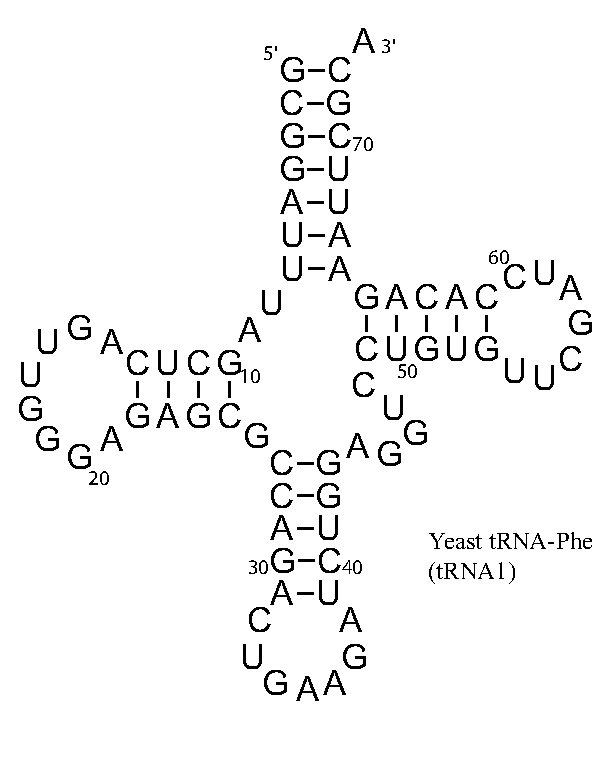
\includegraphics[scale=0.4]{Figures/trna1-DF6280}
\end{minipage}
\vspace{1em}

This is a simple example of a multiple RNA sequence alignment with
secondary structure annotation, in \emph{Stockholm format}.  Stockholm
format, the native alignment format used by HMMER and Infernal and the
Pfam and Rfam databases, is documented in detail later in the guide in
section~\ref{section:formats}.

For now, what you need to know about the key features of the input file is:
\begin{itemize}
\item The alignment is in an interleaved format.
Lines consist of a name, followed by an aligned sequence;
long alignments are split into blocks separated by blank lines.
\item Each sequence must have a unique name that has zero spaces in it. (This is important!)
\item For residues, any one-letter IUPAC nucleotide code is accepted,
      including ambiguous nucleotides. Case is ignored; residues
      may be either upper or lower case.
\item Gaps are indicated by the characters \otext{.}, \otext{\_}, -, or \verb+~+.
      (Blank space is not allowed.)
\item A special line starting with \otext{\#=GC SS\_cons} indicates
      the secondary structure consensus. Gap characters annotate
      unpaired (single-stranded) columns. Base pairs are indicated
      by any of the following pairs: \otext{<>}, \otext{()}, \otext{[]},
      or \otext{\{\}}. No pseudoknots are allowed; the
      open/close-brackets notation is only unambiguous for strictly
      nested base-pairing interactions.
      For more on secondary structure annotation see the WUSS format
      description in section~\ref{section:formats}.
\item The alignment begins with the special tag line
      \otext{\# STOCKHOLM 1.0}, and ends with \otext{//}.
      Stockholm alignments
      can be concatenated to create an alignment database flatfile
      containing many alignments.
\end{itemize}

The \prog{cmbuild} command builds a covariance model from an alignment (or
CMs for each of many alignments in a Stockholm file), and saves the
CM(s) in a file. For example, type:

\user{cmbuild tRNA5.cm tutorial/tRNA5.sto}

and you'll see some output that looks like:

\begin{sreoutput}
# cmbuild :: covariance model construction from multiple sequence alignments
# INFERNAL 1.1.1 (July 2014)
# Copyright (C) 2014 Howard Hughes Medical Institute.
# Freely distributed under the GNU General Public License (GPLv3).
# - - - - - - - - - - - - - - - - - - - - - - - - - - - - - - - - - - - -
# CM file:                                            tRNA5.cm
# alignment file:                                     tutorial/tRNA5.sto
# - - - - - - - - - - - - - - - - - - - - - - - - - - - - - - - - - - - -
#                                                                      rel entropy
#                                                                      -----------
# idx    name                     nseq eff_nseq   alen  clen  bps bifs    CM   HMM description
# ------ -------------------- -------- -------- ------ ----- ---- ---- ----- ----- -----------
       1 tRNA5                       5     3.73     74    72   21    2 0.783 0.489 
#
# CPU time: 0.57u 0.00s 00:00:00.56 Elapsed: 00:00:00.57
\end{sreoutput}

If your input file had contained more than one alignment, you'd get
one line of output for each model. The information on these lines is
almost self-explanatory. The \otext{tRNA5} alignment consisted of 5
%  VERIFY WHEN UPDATING                                           ^
sequences with 74 aligned columns. Infernal turned it into a model of
%              ^^
72 consensus positions, which means it defined 2 gap-containing
%^                                             ^
alignment columns to be insertions relative to consensus. The 5
%                                                             ^
sequences were only counted as an ``effective'' total sequence number
(\otext{eff\_nseq}) of 3.73. The model includes 21 basepairs and 2
%                      ^^^^                     ^^               ^
bifurcations. The model ended up with a relative entropy per position
(\otext{rel entropy, CM}; information content) of 0.783 bits. If the
%                                                 ^^^^^
secondary structure information of the model were ignored the relative
entropy per position (\otext{rel entropy, HMM}) would be 0.489 bits.
%                                                        ^^^^^         
This output format is rudimentary. Infernal knows quite a bit more
information about what it's done to build this CM, but it's not
displaying it. You don't need to know more to be able to use the
model, so we can press on here. Model construction is described in
more detail in section~\ref{section:cmbuild}.

The new CM was saved to \otext{tRNA5.cm}. You can look at it
(e.g. \otext{> more tRNA5.cm}) if you like, but it isn't really designed
to be human-interpretable. You can treat \otext{.cm} files as compiled
models of your RNA alignment. The Infernal ASCII save file format is
defined in Section~\ref{section:formats}.

\subsubsection{Step 2: calibrate the model with cmcalibrate}

The next step is to ``calibrate'' the model. This step must be
performed prior to using your model for database searches with
\prog{cmsearch} or \prog{cmscan}. In this step, statistical parameters
necessary for reporting E-values (expectation values) are estimated
and stored in the CM file. When \prog{cmsearch} or \prog{cmscan} is
later used for a database search and a hit with score $x$ is found,
the E-value of that hit is the number of hits expected to score $x$ or
more just by chance (given the size of the search you're performing).

\emph{Importantly, if you're not going to use a model for database
search, there is no need to calibrate it.} For example, if you are
only going to use a model to create structurally annotated multiple
alignments of a large family like small subunit ribosomal RNA, don't
waste time calibrating it. \prog{cmsearch} and \prog{cmscan} are the
only Infernal programs that use E-values, so if you're not going to
use them then don't calibrate your model.

Unfortunately, CM calibration takes a long time because fairly long
random sequences must be searched to determine the expected
distribution of hit scores against nonhomologous sequences, and none
of the search acceleration heuristics described in
section~\ref{section:pipeline} can be used because they rely on
primary sequence similarity which is absent in random sequence.

The amount of time required for calibration varies widely, but
depends mainly on the size of the RNA family being modeled.
So you can know what kind of a wait you're in for, the
\prog{cmcalibrate} has a \otext{--forecast} option which reports an
estimate of the running time. To get an estimate for the tRNA model, do:

\user{cmcalibrate --forecast tRNA5.cm}\\

You should see something like this:

\begin{sreoutput}
# cmcalibrate :: fit exponential tails for CM E-values
# INFERNAL 1.1.1 (July 2014)
# Copyright (C) 2014 Howard Hughes Medical Institute.
# Freely distributed under the GNU General Public License (GPLv3).
# - - - - - - - - - - - - - - - - - - - - - - - - - - - - - - - - - - - -
# CM file:                                     tRNA5.cm
# forecast mode (no calibration):              on
# - - - - - - - - - - - - - - - - - - - - - - - - - - - - - - - - - - - -
#
# Forecasting running time for CM calibration(s) on 8 cpus:
#
#                          predicted
#                       running time
# model name            (hr:min:sec)
# --------------------  ------------
  tRNA5                     00:06:26
#
# CPU time: 0.27u 0.00s 00:00:00.27 Elapsed: 00:00:00.28
[ok]
\end{sreoutput}

The header comes first, telling you what program you ran, on what file
and with what options. This calibration will use 8 CPUs, your output
may vary depending on how many cores you have available on the machine
you're using. (If you are planning to use MPI to parallelize the
calibration (see the Installation section), you can specify the number
of CPUs for the time estimate as \otext{<n>} with the
\otext{--nforecast <n>} option.) Using 8 CPUs, \prog{cmcalibrate}
estimates the time required for calibration on the machine I'm using
at about seven minutes.

Feel free to perform the calibration yourself if you'd like (with the
command \otext{cmcalibrate tRNA5.cm}). However, we've included the file
\otext{tRNA5.c.cm}, an already calibrated version of \otext{tRNA5.cm},
for you to use if you don't want to wait. To use this calibrated
model, copy over the \otext{tRNA5.cm} file you just made with the
calibrated version:
 
\user{cp tutorial/tRNA5.c.cm tRNA5.cm}\\
 
\subsubsection{Step 3: search a sequence database with cmsearch}

You can now use your tRNA model to search for tRNA homologs in a
database. The file \otext{mrum-genome.fa} is the genome sequence of the
archaeon \emph{Methanobrevibacter rumanitium} (accession:
\otext{NC\_13790.1}). We'll use this file as our database. To perform
the search:

\user{cmsearch tRNA5.cm tutorial/mrum-genome.fa}\\
% tutorial regression: tRNA5-search.out

As before, the first section is the header, telling you what program
your ran, on what, and with what options:

\begin{sreoutput}
# cmsearch :: search CM(s) against a sequence database
# INFERNAL 1.1.1 (July 2014)
# Copyright (C) 2014 Howard Hughes Medical Institute.
# Freely distributed under the GNU General Public License (GPLv3).
# - - - - - - - - - - - - - - - - - - - - - - - - - - - - - - - - - - - -
# query CM file:                         tRNA5.cm
# target sequence database:              tutorial/mrum-genome.fa
# number of worker threads:              8
# - - - - - - - - - - - - - - - - - - - - - - - - - - - - - - - - - - - -
\end{sreoutput}

The second section is a list of ranked top hits (sorted by E-value,
most significant hit first):

\begin{sreoutput}
 rank     E-value  score  bias  sequence      start     end   mdl trunc   gc  description
 ----   --------- ------ -----  ----------- ------- -------   --- ----- ----  -----------
  (1) !   1.3e-18   71.5   0.0  NC_013790.1  362026  361955 -  cm    no 0.50  Methanobrevibacter ruminantium M1 chromosome, complete genome
  (2) !   3.3e-18   70.2   0.0  NC_013790.1 2585265 2585193 -  cm    no 0.60  Methanobrevibacter ruminantium M1 chromosome, complete genome
  (3) !     9e-18   68.8   0.0  NC_013790.1  762490  762562 +  cm    no 0.67  Methanobrevibacter ruminantium M1 chromosome, complete genome
  (4) !     9e-18   68.8   0.0  NC_013790.1 2041704 2041632 -  cm    no 0.67  Methanobrevibacter ruminantium M1 chromosome, complete genome
  (5) !   2.5e-17   67.4   0.0  NC_013790.1 2351254 2351181 -  cm    no 0.62  Methanobrevibacter ruminantium M1 chromosome, complete genome
  (6) !     3e-17   67.2   0.0  NC_013790.1  735136  735208 +  cm    no 0.59  Methanobrevibacter ruminantium M1 chromosome, complete genome
  (7) !   5.2e-17   66.4   0.0  NC_013790.1 2186013 2185941 -  cm    no 0.53  Methanobrevibacter ruminantium M1 chromosome, complete genome
  (8) !   1.6e-16   64.8   0.0  NC_013790.1 2350593 2350520 -  cm    no 0.66  Methanobrevibacter ruminantium M1 chromosome, complete genome
  (9) !   2.8e-16   64.1   0.0  NC_013790.1 2585187 2585114 -  cm    no 0.59  Methanobrevibacter ruminantium M1 chromosome, complete genome
 (10) !   9.1e-16   62.5   0.0  NC_013790.1  662185  662259 +  cm    no 0.61  Methanobrevibacter ruminantium M1 chromosome, complete genome
 (11) !   1.2e-15   62.1   0.0  NC_013790.1  360887  360815 -  cm    no 0.55  Methanobrevibacter ruminantium M1 chromosome, complete genome
 (12) !   1.6e-15   61.7   0.0  NC_013790.1 2350984 2350911 -  cm    no 0.53  Methanobrevibacter ruminantium M1 chromosome, complete genome
 (13) !   3.3e-15   60.7   0.0  NC_013790.1 2186090 2186019 -  cm    no 0.54  Methanobrevibacter ruminantium M1 chromosome, complete genome
 (14) !   4.1e-15   60.4   0.0  NC_013790.1 2680159 2680233 +  cm    no 0.67  Methanobrevibacter ruminantium M1 chromosome, complete genome
 (15) !   7.9e-15   59.5   0.0  NC_013790.1 2749839 2749768 -  cm    no 0.53  Methanobrevibacter ruminantium M1 chromosome, complete genome
 (16) !   7.9e-15   59.5   0.0  NC_013790.1 2749945 2749874 -  cm    no 0.53  Methanobrevibacter ruminantium M1 chromosome, complete genome
 (17) !   9.8e-15   59.2   0.0  NC_013790.1  361676  361604 -  cm    no 0.51  Methanobrevibacter ruminantium M1 chromosome, complete genome
 (18) !     1e-14   59.2   0.0  NC_013790.1 2585073 2584999 -  cm    no 0.60  Methanobrevibacter ruminantium M1 chromosome, complete genome
 (19) !   1.1e-14   59.1   0.0  NC_013790.1 2130422 2130349 -  cm    no 0.59  Methanobrevibacter ruminantium M1 chromosome, complete genome
 (20) !   1.2e-14   58.9   0.0  NC_013790.1  546056  545947 -  cm    no 0.61  Methanobrevibacter ruminantium M1 chromosome, complete genome
 (21) !   3.9e-14   57.3   0.0  NC_013790.1  361915  361844 -  cm    no 0.42  Methanobrevibacter ruminantium M1 chromosome, complete genome
 (22) !   5.1e-14   57.0   0.0  NC_013790.1   97724   97795 +  cm    no 0.49  Methanobrevibacter ruminantium M1 chromosome, complete genome
 (23) !   6.1e-14   56.7   0.0  NC_013790.1 2350717 2350646 -  cm    no 0.68  Methanobrevibacter ruminantium M1 chromosome, complete genome
 (24) !     8e-14   56.3   0.0  NC_013790.1 1873887 1873815 -  cm    no 0.64  Methanobrevibacter ruminantium M1 chromosome, complete genome
 (25) !   1.4e-13   55.6   0.0  NC_013790.1  360730  360659 -  cm    no 0.40  Methanobrevibacter ruminantium M1 chromosome, complete genome
 (26) !   3.5e-13   54.3   0.0  NC_013790.1 2680310 2680384 +  cm    no 0.52  Methanobrevibacter ruminantium M1 chromosome, complete genome
 (27) !   3.6e-13   54.3   0.0  NC_013790.1 2664806 2664732 -  cm    no 0.60  Methanobrevibacter ruminantium M1 chromosome, complete genome
 (28) !   3.6e-13   54.3   0.0  NC_013790.1  361061  360989 -  cm    no 0.41  Methanobrevibacter ruminantium M1 chromosome, complete genome
 (29) !   7.5e-13   53.3   0.0  NC_013790.1 2130335 2130262 -  cm    no 0.55  Methanobrevibacter ruminantium M1 chromosome, complete genome
 (30) !   7.6e-13   53.3   0.0  NC_013790.1 2151672 2151745 +  cm    no 0.65  Methanobrevibacter ruminantium M1 chromosome, complete genome
 (31) !   2.9e-12   51.4   0.0  NC_013790.1  319297  319370 +  cm    no 0.62  Methanobrevibacter ruminantium M1 chromosome, complete genome
 (32) !   3.7e-12   51.1   0.0  NC_013790.1  361753  361679 -  cm    no 0.55  Methanobrevibacter ruminantium M1 chromosome, complete genome
 (33) !   3.8e-12   51.1   0.0  NC_013790.1  360983  360912 -  cm    no 0.50  Methanobrevibacter ruminantium M1 chromosome, complete genome
 (34) !   5.9e-12   50.5   0.0  NC_013790.1  361456  361383 -  cm    no 0.50  Methanobrevibacter ruminantium M1 chromosome, complete genome
 (35) !   7.4e-12   50.1   0.0  NC_013790.1  362798  362727 -  cm    no 0.51  Methanobrevibacter ruminantium M1 chromosome, complete genome
 (36) !   8.7e-12   49.9   0.0  NC_013790.1  917722  917793 +  cm    no 0.61  Methanobrevibacter ruminantium M1 chromosome, complete genome
 (37) !   1.1e-11   49.7   0.0  NC_013790.1 2583869 2583798 -  cm    no 0.51  Methanobrevibacter ruminantium M1 chromosome, complete genome
 (38) !   1.3e-11   49.4   0.0  NC_013790.1  362324  362252 -  cm    no 0.51  Methanobrevibacter ruminantium M1 chromosome, complete genome
 (39) !   1.3e-11   49.3   0.0  NC_013790.1  360811  360740 -  cm    no 0.42  Methanobrevibacter ruminantium M1 chromosome, complete genome
 (40) !   4.3e-11   47.7   0.0  NC_013790.1 1160526 1160609 +  cm    no 0.60  Methanobrevibacter ruminantium M1 chromosome, complete genome
 (41) !   9.8e-11   46.6   0.0  NC_013790.1  362403  362331 -  cm    no 0.49  Methanobrevibacter ruminantium M1 chromosome, complete genome
 (42) !   1.1e-10   46.5   0.0  NC_013790.1 2327124 2327042 -  cm    no 0.63  Methanobrevibacter ruminantium M1 chromosome, complete genome
 (43) !   1.2e-10   46.4   0.0  NC_013790.1  995344  995263 -  cm    no 0.49  Methanobrevibacter ruminantium M1 chromosome, complete genome
 (44) !   2.3e-10   45.5   0.0  NC_013790.1  256772  256696 -  cm    no 0.57  Methanobrevibacter ruminantium M1 chromosome, complete genome
 (45) !   2.5e-10   45.3   0.0  NC_013790.1 2584830 2584758 -  cm    no 0.64  Methanobrevibacter ruminantium M1 chromosome, complete genome
 (46) !   6.1e-10   44.1   0.0  NC_013790.1 2351071 2350997 -  cm    no 0.59  Methanobrevibacter ruminantium M1 chromosome, complete genome
 (47) !   6.5e-10   44.0   0.0  NC_013790.1  362552  362482 -  cm    no 0.55  Methanobrevibacter ruminantium M1 chromosome, complete genome
 (48) !   5.2e-09   41.2   0.0  NC_013790.1 1064775 1064858 +  cm    no 0.63  Methanobrevibacter ruminantium M1 chromosome, complete genome
 (49) !   1.2e-08   40.0   0.0  NC_013790.1  361222  361150 -  cm    no 0.45  Methanobrevibacter ruminantium M1 chromosome, complete genome
 (50) !   1.2e-08   40.0   0.0  NC_013790.1  361369  361297 -  cm    no 0.60  Methanobrevibacter ruminantium M1 chromosome, complete genome
 (51) !   4.8e-08   38.1   0.0  NC_013790.1  361596  361513 -  cm    no 0.61  Methanobrevibacter ruminantium M1 chromosome, complete genome
 (52) !   3.2e-07   35.5   0.0  NC_013790.1 1913310 1913227 -  cm    no 0.64  Methanobrevibacter ruminantium M1 chromosome, complete genome
 (53) !   2.6e-06   32.7   0.0  NC_013790.1  363464  363381 -  cm    no 0.51  Methanobrevibacter ruminantium M1 chromosome, complete genome
 (54) !     3e-06   32.5   0.0  NC_013790.1 2584954 2584872 -  cm    no 0.58  Methanobrevibacter ruminantium M1 chromosome, complete genome
 ------ inclusion threshold ------
 (55) ?     0.027   20.0   0.0  NC_013790.1  363803  363716 -  cm    no 0.50  Methanobrevibacter ruminantium M1 chromosome, complete genome
 (56) ?       3.4   13.4   0.0  NC_013790.1  984373  984304 -  cm    no 0.53  Methanobrevibacter ruminantium M1 chromosome, complete genome
\end{sreoutput}

The first number is the rank of each hit\footnote{Ranks of hits are in
  parantheses to make it easy to jump to/from an entry in the hit list
  and the hit alignment section, described later.}. Next comes either a
\otext{!} or \otext{?} symbol and then the \emph{E-value} of the hit.
The E-value is the statistical significance of the hit: the number of
hits we'd expect to score this highly in a database of this size
(measured by the total number of nucleotides) if the database
contained only nonhomologous random sequences. The lower the E-value,
the more significant the hit. The \otext{!} or \otext{?} that
precedes the E-value indicates whether the hit does (\otext{!}) or
does not (\otext{?}) satisfy the inclusion threshold for the search.
Inclusion thresholds are used to determine what matches should be
considered to be ``true'', as opposed to reporting thresholds that
determine what matches will be reported (often including the top of
the noise, so you can see what interesting sequences might be getting
tickled by your search). By default, inclusion thresholds usually
require an E-value of 0.01 or less, and reporting E-value thresholds
are set to 10.0, but these can be changed (see the manual page for
\prog{cmsearch} toward the end of guide).

The E-value is based on the \emph{bit score}, which is in the next
column. This is the log-odds score for the hit. Some people like to
see a bit score instead of an E-value, because the bit score doesn't
depend on the size of the sequence database, only on the covariance
model and the target sequence.

The next number, the \emph{bias}, is a correction term for biased
sequence composition that has been applied to the sequence bit
score. Infernal uses an alternative null model we call \emph{null3},
described more in section~\ref{section:pipeline}, to determine the bias
bit score correction. The bias correction is often very small and is
only reported to one decimal place, after rounding. For all hits in
this example search the bias column reads 0.0 bits, indicating that
the correction is less than 0.05 bits. On very biased sequences this
correction can become significant and is helpful for lowering the
score of high-scoring false positives that achieve high scores solely
due to their biased composition. 

Next comes the target sequence name the hit is in, and the start and
end positions of the hit within the sequence. Hits can occur on either
the top (Watson) or bottom (Crick) strand of the target
sequence\footnote{You can search either only the top strand with the
\otext{--toponly} or bottom strand with the \otext{--bottomonly} options
to \prog{cmsearch} and \prog{cmscan}.}, so the start position may be
less than (if hit is on the top strand) or greater than (if hit is on
the bottom strand) the end position. After the end position, comes a single
\otext{+} or \otext{-} symbol, indicating whether the hit is on the
top (\otext{+}) or bottom (\otext{-}) strand (solely for convenience -
so you don't have to look at the start and end positions to determine
the strand the hit is on).

After the strand symbol comes the model field, which indicates whether
the hit was found using either the CM (\otext{cm}) or a profile HMM
built from the CM (\otext{hmm}). This field is necessary because for
models with zero basepairs, \prog{cmsearch} (and \prog{cmscan}) use a
profile HMM instead of a CM for final hit scoring. This is done for
reasons of speed and efficiency, because profile HMM algorithms are
more efficient than CM ones and a CM with zero basepairs is
essentially equivalent to a profile HMM. In this example, since our
tRNA model does include basepairs, \prog{cmsearch} used a CM to score
all hits and so all hits have \prog{cm} for this column. There's an
example later in the tutorial of hits found with a profile HMM.

The next column indicates whether the hit is \emph{truncated} or
not. Infernal uses special versions of its CM dynamic programming
algorithms to allow detection of structural RNAs that have been
truncated due to missing data at the beginning and/or end of a target
sequence. Truncated hits are most common in databases that include
single reads from shotgun sequencing projects. Since our database is a
complete genome, we don't expect any hits to be truncated due to
missing data. For all hits the ``trunc'' column reads
``no'' indicating that, as expected, none of the hits are
truncated. There are examples of truncated hits in the next exercise
which uses \prog{cmscan}. Section~\ref{section:pipeline} describes how
Infernal detects and aligns truncated hits in more detail.

The next column reports the GC fraction of the hit. This is the
fraction of residues in the target sequence hit that are either G or C
residues. The GC fraction is included as an additional indication of
the level of sequence bias of the hit. Some expert users may be aided
by this number when deciding if they believe a hit is a real homolog
or a false positive.

Finally comes the description of the sequence, if any. This
description is propogated from the input target sequence file.

After the hit list comes the hit alignments section. Each hit in 
the hit list will have a corresponding entry in this section, in the
same order. As an illustrative example, let's take a look at
hit number 43. First, take a look at the first four lines for this
hit: 

\begin{sreoutput}
>> NC_013790.1  Methanobrevibacter ruminantium M1 chromosome, complete genome
 rank     E-value  score  bias mdl mdl from   mdl to       seq from      seq to       acc trunc   gc
 ----   --------- ------ ----- --- -------- --------    ----------- -----------      ---- ----- ----
 (43) !   1.2e-10   46.4   0.0  cm        1       72 []      995344      995263 - .. 0.93    no 0.49
\end{sreoutput}

The first line of each hit alignment begins with \otext{>>} followed
by a single space, the name of the target sequence, then two spaces
and the description of the sequence, if any. Next comes a set of
tabular fields that is partially redundant with the information in the
hit list. The first five columns are the same as in the hit list. The
next column reports the type of model used for the alignment, as
described above for the hit list. The next four columns report the
boundaries of the alignment with respect to the query model (``mdl
from'' and ``mdl to'') and the target sequence (``seq from'' and ``seq
to''). Following the ``seq to'' column is a \otext{+} or \otext{-}
symbol indicating whether the hit is on the top (\otext{+}) or bottom
(\otext{-}) strand.

It's not immediately easy to tell from the ``to'' coordinate whether
the alignment ended internally in the query model or target sequence,
versus ran all the way (as in a full-length global alignment) to the
end(s). To make this more readily apparent, with each pair of query
and target endpoint coordinates, there's also a little symbology. For
the normal case of a non-truncated hit: \otext{..} means both ends of
the alignment ended internally, and \otext{[]} means both ends of the
alignment were full-length flush to the ends of the query or target,
and \otext{[.}  and \otext{.]} mean only the left (5') or right (3') end
was flush/full length. For truncated hits, the symbols are the same
except that either the first and/or the second symbol will be a
\verb+~+ for the query and target. If the first symbol is \verb+~+
then the left end of the alignment is truncated because the 5' end of
the hit is predicted to be missing (extend beyond the beginning of the
target sequence). Similarly, if the second symbol is \verb+~+ then the
right end of the alignment is truncated because the 3' end of the hit
is predicted to be missing (extend beyond the end of the target
sequence). These two symbols occur just after the ``mdl to'' column for
the query, and after the strand \otext{+} or \otext{-} symbol for the
target sequence.

The next column is labeled ``acc'' and is the average posterior
probability of the aligned target sequence residues; effectively, the
expected accuracy per residue of the alignment.

The final two columns indicate whether the hit is truncated or not and
the GC fraction of the hit. These are redundant with the columns of
the same name in the hit list, described above.

Next comes the alignment display. This is an ``optimal
posterior accuracy'' alignment \citep{Holmes98}, which means it is the
alignment with the maximal summed posterior probability of all
aligned residues. Take a look at the alignment for hit number 43:

% tutorial regression: tRNA5-search.out
\begin{sreoutput}
                                 v         v                                                            NC
                     (((((((,,<<<<______.._>>>>,<<<<<_______>>>>>,,,........,,<<<<<_______>>>>>))))))): CS
        tRNA5      1 gCcggcAUAGcgcAgUGGu..AgcgCgccagccUgucAagcuggAGg........UCCgggGUUCGAUUCcccGUgccgGca 72    
                     :::G:CAUAGCG AG GGU  A CGCG:CAG:CU +++A:CUG: G+        UC:GGGGUUCGA UCCCC:UG:C:::A
  NC_013790.1 995344 AGAGACAUAGCGAAGCGGUcaAACGCGGCAGACUCAAGAUCUGUUGAuuaguucuUCAGGGGUUCGAAUCCCCUUGUCUCUA 995263
                     **********************************************9444444445************************** PP
\end{sreoutput}

The alignment contains six lines. Start by looking at the second line
which ends with \otext{CS}.  The line shows the predicted secondary
structure of the target sequence. The format is a little fancier and
more informative than the simple least-common-denominator format we
used in the input alignment file. It's designed to make it easier to
see the secondary structure by eye. The format is described in detail
later (see WUSS format in section~\ref{section:formats}); for now,
here's all you need to know. Basepairs in simple stem loops are
annotated with \otext{<>} characters. Basepairs enclosing
multifurcations (multiple stem loops) are annotated with \otext{()},
such as the tRNA acceptor stem in this example. In more complicated
structures, \otext{[]} and \otext{\{\}} annotations also show up, to
reflect deeper nestings of multifurcations. For single stranded
residues, \otext{\_} characters mark hairpin loops; \otext{-}
characters mark interior loops and bulges; \otext{,} characters mark
single-stranded residues in multifurcation loops; and \otext{:}
characters mark single stranded residues external to any secondary
structure. Insertions relative to this consensus are annotated by a
\otext{.} character.

The line above the \otext{CS} line ends with \otext{NC} and marks
negative scoring non-canonical basepairs in the alignment with a
\otext{v} character. All other positions of the alignment will be
blank\footnote{For anyone trying to parse this output, this means it
is possible for this line to be completely blank except for the
\otext{NC} trailer.} More specifically, the following ten types of
basepairs which are assigned a negative score by the model at their
alignment positions will be marked with a \otext{v}: \otext{A:A},
\otext{A:C}, \otext{A:G}, \otext{C:A}, \otext{C:C}, \otext{C:U},
\otext{G:A}, \otext{G:G}, \otext{U:U}, and \otext{U:C}. The \otext{NC}
annotation makes it easy to quickly identify suspicious basepairs in
a hit. Importantly, the \otext{NC} annotation will only be present in
CM hit alignments (``mdl'' column reads ``cm'') and will be absent in
HMM hit alignments (``mdl'' column reads ``hmm'') because basepairs
are not scored by an HMM.

The third line shows that consensus of the query model. The highest
scoring residue sequence is shown. Upper case residues are highly
conserved. Lower case residues are weakly conserved or unconserved.
Dots (\otext{.}) in this line indicate insertions in the target
sequence with respect to the model.

The fourth line shows where the alignment score is coming from. For a
consensus basepair, if the observed pair is the highest-scoring
possible pair according to the consensus, both residues are shown in
upper case; if a pair has a score of $\geq 0$, both residues are
annotated by : characters (indicating an acceptable compensatory
basepair); else, there is a space, indicating that a negative
contribution of this pair to the alignment score. Note that the 
\otext{NC} line will only mark a subset of these negative scoring
pairs with a \otext{v}, as discussed above.
For a single-stranded consensus residue, if the observed residue is
the highest scoring possibility, the residue is shown in upper case;
if the observed residue has a score of $\geq 0$, a \otext{+} character
is shown; else there is a space, indicating a negative contribution to
the alignment score. Importantly, for HMM hits (``mdl'' column reads
``hmm''), \emph{all} positions are considered single stranded, since
an HMM scores each half of a basepair independently.

The fifth line, beginning with \otext{NC\_013790.1} is
the target sequence. Dashes (\otext{-}) in this line indicate deletions
in the target sequence with respect to the model.

The bottom line is new to version 1.1 of Infernal. This represents the
posterior probability (essentially the expected accuracy) of each
aligned residue. A 0 means 0-5\%, 1 means 5-15\%, and so on; 9 means
85-95\%, and a \otext{*} means 95-100\% posterior probability. You can
use these posterior probabilities to decide which parts of the
alignment are well-determined or not. You'll often observe, for
example, that expected alignment accuracy degrades around locations of
insertion and deletion, which you'd intuitively expect.

Alignments for some searches may be formatted slightly differently
than this example. Longer alignments to longer models will be broken
up into blocks of six lines each - this alignment was short enough to
be entirely contained within a single block.  If your model was built
with the \otext{--hand} option in \prog{cmbuild}, then an additional
line will be included in each block, with RF annotation.  If the model
used for the alignment was an HMM (the ``mdl'' column reads ``hmm'')
then the \otext{NC} line will be absent from each alignment
block. We'll see example of all three of these cases later in the
tutorial.

After hit number 43, there's 13 more hit alignments for hits number 44
through 56. 

Finally, at the bottom of the file, you'll see some summary
statistics. For example, at the bottom of the tRNA search output,
you'll find something like:

\begin{sreoutput}
Internal CM pipeline statistics summary:
----------------------------------------
Query model(s):                                                  1  (72 consensus positions)
Target sequences:                                                1  (5874406 residues searched)
Target sequences re-searched for truncated hits:                 1  (360 residues re-searched)
Windows   passing  local HMM SSV           filter:           11200  (0.2111); expected (0.35)
Windows   passing  local HMM Viterbi       filter:                  (off)
Windows   passing  local HMM Viterbi  bias filter:                  (off)
Windows   passing  local HMM Forward       filter:             137  (0.002691); expected (0.005)
Windows   passing  local HMM Forward  bias filter:             134  (0.002621); expected (0.005)
Windows   passing glocal HMM Forward       filter:              87  (0.001923); expected (0.005)
Windows   passing glocal HMM Forward  bias filter:              87  (0.001923); expected (0.005)
Envelopes passing glocal HMM envelope defn filter:             100  (0.001342); expected (0.005)
Envelopes passing  local CM  CYK           filter:              60  (0.0007631); expected (0.0001)
Total CM hits reported:                                         56  (0.0007205); includes 0 truncated hit(s)

# CPU time: 2.15u 0.03s 00:00:02.17 Elapsed: 00:00:00.89
//
[ok]
\end{sreoutput}

This gives you some idea of what's going on in Infernal's acceleration
pipeline. You've got one query CM, and the database has one target
%                    ^                                  ^
sequence. The search examined 5,874,406 residues, even though the
%                             ^^^^^^^^^
actual target sequence length is only half that, because both the top
and bottom strand of each target is searched. 360 of those residues
%                                             ^^^
were searched more than once in an effort to find truncated
hits. Ignore this for the moment, we'll revisit this later after
discussing the filter pipeline (in the subsection entitled ``Truncated
RNA detection'' below).

Each sequence goes through a multi-stage filter pipeline of four
scoring algorithms called SSV, Viterbi, Forward\footnote{Actually two
  separate Forward based filters are used, the first with the profile
  HMM in local mode and the next with the profile HMM in global
  mode. There's more detail on this in
  section~\ref{section:pipeline}.}, and CYK in order of increasing
sensitivity and increasing computational requirement. The filter
pipeline is the topic of section~\ref{section:pipeline} of this guide
but briefly, SSV, Viterbi and Forward are profile HMM algorithms which
are more efficient than CM algorithms. These three algorithms are the
same ones used by HMMER3 and are the main reason that version 1.1 of
Infernal is so much faster than previous versions. For these HMM
stages, Infernal uses a filter profile HMM that was constructed
simultaneously with the CM, from the same training alignment in
\prog{cmbuild}, and stored in the CM file. CYK is a CM scoring
algorithm, so it's slow, but it is accelerated using banded dynamic
programming with bands derived from an HMM alignment. Subsequences
that survive all filters are finally scored with the CM Inside
algorithm, agains using HMM bands. Subsequences that score
sufficiently high with Inside are then aligned using the optimal
posterior accuracy algorithm and displayed.

The score thresholds for a subsequence surviving each HMM filter stage
are dependent on the search space size (sequence database size for
\prog{cmsearch}). This differs from HMMER3 which always uses the same
filter thresholds. In general, the larger the search
space the more strict the thresholds are, because a hit must have a
higher bit score to have a significant E-value.  In this case, the
database is relatively small so the filter thresholds have been set
relatively loosely. The SSV filter has been configured to allow
subsequences with a P-value of $\leq 0.35$ through
%                                   ^^^^^^
the SSV score filter (thus, if the database contained no homologs and
P-values were accurately calculated, the highest scoring 35\% of the
%                                           ^^^^
residues will pass the filter). Here, about 21\% of the database in
%                                           ^^^^
11,200 separate windows got through the SSV filter. For a database of
%^^^^^
this size, the local Viterbi filter is turned off.  The local Forward filter
is set to allow an expected 0.5\% of the database survive. Here about
%                           ^^^^
0.3\% survives in 137 windows. Next, each surviving window is checked
%^^
to see if the target sequence is ``obviously'' so biased in its
composition that it's unlikely to be a true homolog. This is called
the ``bias filter''\footnote{There's also a bias filter step used in
  the local Viterbi filter stage, when it is used.} and applying a bit
score correction to previous filter's score for each window and
recomputing the P-value. Three of the 137 windows fail to pass
%                        ^^^^^        ^^^
the local Forward bias filter stage. Next, the Forward algorithm is
used to score each window again, but this time with the HMM configured
in glocal mode requiring a full length alignment to the
model\footnote{The use of glocal Forward is another important
  difference between Infernal and HMMER3's (v3.0) pipeline. HMMER v3.0
  only uses local HMM algorithms.}  As with the local stage, an
expected 0.5\% of the database is expected to survive. In this case,
87 of the 134 windows, comprising about 0.2\% of the database,
%^        ^^^
survive. The bias filter is run again, this time applying a correction
to the glocal Forward scores. For this search, 0 windows are removed at
this stage. The envelope definition stage is next. This stage is very
similar to the HMMER3 domain definition stage, with the difference
that the HMM is configured in glocal rather than local mode. In this
stage, the Forward and Backward algorithms are used to identify zero
or more hit envelopes in each window, where each envelope contains one
putative hit.  Often residues at the beginning and ends of windows are
determined to be nonhomologous and are not included in the
envelope. In this search, 100 envelopes are defined within the 87
%                         ^^^                                  ^^
windows. Note that the envelopes comprise only about 70\% of the
%                                                    ^^^
residues from the 87 windows, indicated by the drop of 0.1923\% to
%                                                      ^^^^^^^^
0.1342\%.
%%^^^^

After hit envelopes have been defined with the filter HMM, the two
remaining stages of the pipeline use the CM to score both the
conserved sequence and structure of each possible hit. In both of
these stages, constraints are derived from an HMM alignment of the
envelope and enforced as \emph{bands} on the CM dynamic programming
matrices (more on this in section~\ref{section:pipeline}). In the
first CM stage, the CYK algorithm (which is the SCFG analog of the
Viterbi HMM algorithm) is used to determine the best scoring maximum
likelihood alignment of any subsequence in each envelope to the CM. If
this alignment has a P-value of $\leq 0.0001$ then the envelope
survives to the final round. The envelopes passed to the final stage
may be shorter than those examined during the CYK stage. Specifically,
envelopes are redefined as starting and ending at the first and final
residues for which at least one alignment exists with a P-value $\leq
0.001$.

In the final round, the Inside algorithm (the SCFG analog of the HMM
Forward algorithm) is used to define final hit boundaries and
scores. Hits with scores above the reporting threshold were output, as
described above. In this search there were 56 such hits.
%                                          ^^

Finally, the running time of the search is reported, in CPU time and
elapsed time. This search took about 1 second (wall
%                                    ^
clock time) (running on eight cores). 

\subsubsection{Truncated RNA detection}

Now, we come back to the topic of truncated hit detection.  As briefly
mentioned above, the pipeline statistics summary from our search above
reported that 360 residues were re-searched for truncated
%             ^^^
hits. Infernal explicitly looks at the 5' and 3' ends of target
sequences using specialized algorithms for detection of truncated
hits, in which part of the 5' and/or 3' end of the actual full length
sequence from the source organism's full genomic context is missing in
the input target sequence. Truncated hits will be most common in
sequence files consisting of unassembled sequencing reads. In our
search of the full archaeal genome above, no truncated hits were
found. However, there is an example of a truncated hit in the
\prog{cmscan} tutorial section below in a sequence from a metagenomics
sequencing survey.

Special dynamic programming algorithms are required for truncated hit
detection \citep{KolbeEddy09}, so sequences must be re-searched for
truncated hits after they are initially searched for standard
(non-truncated) hits. However, only the sequence ends must be
re-searched because Infernal assumes that only hits at sequence
terminii might be truncated. This is why our search above reported
that only 360 residues were re-searched for truncated hits. For each
%         ^^^
model, an expected maximum length of a hit\footnote{The expected
  maximum hit length is defined as the maximum of 1.25 times the
  consensus length of the model and the $W$ parameter computed with
  the QDB algorithm \citep{NawrockiEddy07}. $W$ is computed based on
  the transition probabilities of the model by \prog{cmbuild} and
  stored in the CM file.} 
is used to define the window length at the
beginning and end of each sequence which must be re-searched for
truncated hits. For our tRNA model the maximum expected length is
90, so exactly 360 residues were re-searched: the first and final 90
%^             ^^^                                                ^^
residues on the top strand, and the first and final 90 residues on
%                                                   ^^
the bottom strand.

There is one more aspect of truncated hit detection that is important
to mention here. Because Infernal expects that hit truncation only
occurs at the ends of sequences, 5' truncated hits are forced to start
at the first nucleotide of a sequence, 3' truncated hits are forced to
end at the final nucleotide of the sequence, and 5' \emph{and} 3'
truncated hits are forced to include the full sequence.

The annotation of truncated hits in \prog{cmsearch} output is slightly
different than for standard (non-truncated) hits. An example is
included in the next section below.

\subsection{Searching a CM database with a query sequence}

The \prog{cmscan} program is for annotating all the different
known/detectable RNAs in a given sequence. It takes a single query
sequence and a CM database as input. The CM database might be Rfam,
for example, or another collection of your choice. \prog{cmscan} is
new to version 1.1 of Infernal. It is designed to be useful for
sequence datasets from RNA-Seq experiments or metagenomics surveys,
for which one wants to know what families of RNAs are represented in
the sequence dataset.

\subsubsection{Step 1: create an CM database flatfile}

A CM ``database'' flatfile is simply a concatenation of individual CM
files. To create a database flatfile, you can either build and
calibrate individual CM files and concatenate them, or you can
concatenate Stockholm alignments and use \prog{cmbuild} to build a CM
database of all of them in one command, and then calibrate that
database with \prog{cmcalibrate}. Importantly, \prog{cmscan} can only
be used with calibrated CMs.

Let's create a tiny database called \otext{minifam.cm} containing the
tRNA model we've been working with, a 5S ribosomal RNA model, and a
Cobalamin riboswitch model. To save you time, calibrated versions of
the 5S and Cobalamin models are included in the \otext{tutorial/}
directory in the files \otext{5S\_rRNA.c.cm}, and
\otext{Cobalamin.c.cm}. These files were created using \prog{cmbuild}
and \prog{cmcalibrate} from the Rfam 10.1 seed alignments for 5S\_rRNA
(RF00001) and Cobalamin (RF00174), provided in
\otext{tutorial/5S\_rRNA.sto} and \otext{tutorial/Cobalamin.sto}. The
third model is the tRNA model from earlier in the tutorial 
(\otext{tRNA5.c.cm}). Feel free to build and calibrate these
models yourself if you'd like, but if you'd like to keep moving on
with the tutorial, use the pre-calibrated ones. To create the database,
simply concatenate the three provided files:

\user{cat tutorial/tRNA5.c.cm tutorial/5S\_rRNA.c.cm tutorial/Cobalamin.c.cm > minifam.cm}

\subsubsection{Step 2: compress and index the flatfile with cmpress}

The \prog{cmscan} program has to read a lot of CMs and their filter
HMMs in a hurry, and Infernal's ASCII flatfiles are bulky. To
accelerate this, \prog{cmscan} uses binary compression and indexing of
the flatfiles. To use \prog{cmscan}, you must first compress and
index your CM database with the \prog{cmpress} program:

\user{cmpress minifam.cm}

This will quickly produce:

\begin{sreoutput}
Working...    done.
Pressed and indexed 3 CMs and p7 HMM filters (3 names and 2 accessions).
Covariance models and p7 filters pressed into binary file:  minifam.cm.i1m
SSI index for binary covariance model file:                 minifam.cm.i1i
Optimized p7 filter profiles (MSV part)  pressed into:      minifam.cm.i1f
Optimized p7 filter profiles (remainder) pressed into:      minifam.cm.i1p
\end{sreoutput}

and you'll see these four new binary files in the directory. 

The \otext{tutorial} directory includes a copy of the
\otext{minifam.cm} file, which has already been pressed, so there
are example binary files \otext{tutorial/minifam.cm.i1\{m,i,f,p\}}
included in the tutorial.

Their format is ``proprietary'', which is an open source term of art
that means both ``We haven't found time to document them yet'' and ``We
still might decide to change them arbitrarily without telling you''.

\subsubsection{Step 3: search the CM database with cmscan}

Now we can analyze sequences using our CM database and
\prog{cmscan}. 

For example, the file \otext{tutorial/metag-example.fa} includes 3
sequences (whole genome shotgun sequencing reads) derived from samples
of ``whale fall'' carcasses in a metagenomics study
\citep{Tringe05}. These three sequences were chosen from the roughly
200,000 in the complete dataset because they include statistically
significant hits to the three models in our toy CM database.

To scan the sequences with our database: 

\user{cmscan minifam.cm tutorial/metag-example.fa}
%tutorial regression: metag-scan.out

The header and the first section of the output will look like:

\newpage

\begin{sreoutput}
# cmscan :: search sequence(s) against a CM database
# INFERNAL 1.1.1 (July 2014)
# Copyright (C) 2014 Howard Hughes Medical Institute.
# Freely distributed under the GNU General Public License (GPLv3).
# - - - - - - - - - - - - - - - - - - - - - - - - - - - - - - - - - - - -
# query sequence file:                   ../../tutorial/metag-example.fa
# target CM database:                    minifam.cm
# number of worker threads:              8
# - - - - - - - - - - - - - - - - - - - - - - - - - - - - - - - - - - - -

Query:       AAGA01015927.1  [L=943]
Description: Metagenome sequence AHAI1002.g1, whole genome shotgun sequence
Hit scores:
 rank     E-value  score  bias  modelname  start    end   mdl trunc   gc  description
 ----   --------- ------ -----  --------- ------ ------   --- ----- ----  -----------
  (1) !   3.3e-19   77.3   0.0  5S_rRNA       59    174 +  cm    no 0.66  5S ribosomal RNA
  (2) !   9.3e-19   62.4   0.0  tRNA5        229    302 +  cm    no 0.62  -
  (3) !     6e-16   53.5   0.0  tRNA5        314    386 +  cm    no 0.59  -
\end{sreoutput}

\prog{cmscan} has identified three putative RNAs in the first query
sequence, one 5S rRNA and two tRNAs. The output fields are in the
same order and have the same meaning as in \prog{cmsearch}'s output.

Before we move on, this is a good opportunity to point out an
important difference between \prog{cmsearch} and \prog{cmscan} related
to the size of the search space (often referred to in the code and in
this guide as the $Z$ parameter).  The size of the search space for
\prog{cmscan} is double the length of the current (single) query
sequence (doubled because we're searching both strands) multiplied by
the number of models in the CM database (here, 3; for a Rfam search,
on the order of 1000). Because each query sequence is probably a
different size this means $Z$ changes for each query sequence. In
\prog{cmsearch}, the size of the search space is double the summed
length of all sequences in the database (again, doubled because both
strands are searched). This means that E-values may differ even for
the same individual CM vs. sequence comparison, depending on how you
do the search. The search space size also affects what filter
thresholds \prog{cmsearch} or \prog{cmscan} will use, which is
discussed more in section~\ref{section:pipeline}.

Now back to the \prog{cmscan} results. What follows the ranked list of
three hits are the hit alignments. These are constructed and annotated
the same as in \prog{cmsearch}. The 5S alignment is:

\begin{widesreoutput}
                             v               v       v         v         v             v           vv                NC
                     (((((((((,,,,<<-<<<<<---<<--<<<<<<______.>>-->>>>-->>---->>>>>-->><<<-<<----<-<<-----<<____>>-- CS
         5S_rRNA   1 gcuuGcggcCAUAccagcgcgaAagcACcgGauCCCAUCc.GaACuCcgAAguUAAGcgcgcUugggCcagggUAGUAcuagGaUGgGuGAcCuC 94 
                     :CU:GC:G C UA:C+::G:G+   CACC:GA CCCAU C G ACUC:GAAG  AA C:C::U+G: CC+::G  G:A  + G  GGGU  CC C
  AAGA01015927.1  59 CCUGGCGGCCGUAGCGCGGUGGUCCCACCUGACCCCAUGCcGAACUCAGAAGUGAAACGCCGUAGCGCCGAUG--GUAGUGUG--GGGUCUCCCC 149
                     *************************************************************************..********..********** PP

                        vv         v v          NC
                     --->>->-->>->>>.))))))))): CS
         5S_rRNA  95 cUGggAAgaccagGu.gccgCaagcc 119
                      UG  A: A::AGG   C:GC:AG:C
  AAGA01015927.1 150 AUGCGAG-AGUAGGGaACUGCCAGGC 174
                     **99999.****************** PP
\end{widesreoutput}

After the three sequences, you'll see a pipeline statistics summary
report:

\begin{widesreoutput}
Internal CM pipeline statistics summary:
----------------------------------------
Query sequence(s):                                               1  (1886 residues searched)
Query sequences re-searched for truncated hits:                  1  (992.0 residues re-searched, avg per model)
Target model(s):                                                 3  (382 consensus positions)
Windows   passing  local HMM SSV           filter:              16  (0.3323); expected (0.35)
Windows   passing  local HMM Viterbi       filter:                  (off)
Windows   passing  local HMM Viterbi  bias filter:                  (off)
Windows   passing  local HMM Forward       filter:               4  (0.09822); expected (0.02)
Windows   passing  local HMM Forward  bias filter:               4  (0.09822); expected (0.02)
Windows   passing glocal HMM Forward       filter:               3  (0.09822); expected (0.02)
Windows   passing glocal HMM Forward  bias filter:               3  (0.09822); expected (0.02)
Envelopes passing glocal HMM envelope defn filter:               4  (0.05189); expected (0.02)
Envelopes passing  local CM  CYK           filter:               4  (0.05189); expected (0.0001)
Total CM hits reported:                                          3  (0.03046); includes 0 truncated hit(s)

# CPU time: 0.21u 0.01s 00:00:00.22 Elapsed: 00:00:00.22
//
\end{widesreoutput}

This report is similar to the one you saw earlier from
\prog{cmsearch}, but not identical. One big difference is that
\prog{cmscan} will report a summary per query sequence, instead of per
query model. In this case, the sequence was 943 residues long, so a
%                                           ^^^
total of 1886 residues were searched, since both strands were
%        ^^^^
examined. The next line reports that the average number of residues
re-searched for truncated hits per model was 992.0. An average is
%                                            ^^^^^
reported here because remember the number of residues re-searched per
model depends on the expected maximum size of a hit, which varies per
model, because only sequence terminii are examined for truncated hits
(see ``Truncated RNA detection'' above and
section~\ref{section:pipeline}).  The remainder of the output is the
same as in \prog{cmsearch} except that the fractional values are
averages per model. For example, for all three models a total of 4
envelopes survived the CYK filter stage, and those surviving envelopes
contained 5.189\% of the target sequence \emph{on average per model}.

You may have noticed that the expected survival fractions are
different than they were in the \prog{cmsearch} example. This is
because the P-value filter thresholds are set differently depending on
the search space. For this example, the search space ($Z$) is roughly
only 6 Kb (1886 residues in the query sequence multiplied by 3 target
models), so the thresholds are set differently than for the
\prog{cmsearch} example which had a search space size of roughly 6
Mb. The exact thresholds used for various $Z$ values can be found in
Table~\ref{tbl:thresholds} in section~\ref{section:pipeline}.

\subsubsection{Truncated hit and local end alignment example}
Next, take a look at the \prog{cmscan} output for the second query
sequence \otext{AAFY01022046.1}. The bottom strand of this sequence
contains one hit to the Cobalamin riboswitch model, which is truncated
at the 5' end. Here is the alignment:

\begin{widesreoutput}
Hit alignments:
>> Cobalamin  Cobalamin riboswitch
 rank     E-value  score  bias mdl mdl from   mdl to       seq from      seq to       acc trunc   gc
 ----   --------- ------ ----- --- -------- --------    ----------- -----------      ---- ----- ----
  (1) !   6.1e-09   30.0   0.0  cm       32      191 ~]         934         832 - ~. 0.92    5' 0.48

                                 ???              v           v      v    v                                     ???? NC
                     ~~~~~~______>>>,,,,,(((,,,<.<<<<_______>>>>>,,<<<____>>>,<<<---<<<<~~~~~~>>>>---->>>,,,,)))]]]] CS
       Cobalamin   1 <[31]*agugaaggguuAAaaGGGAAc.ccGGUGaaAaUCCgggGCuGcCCCCgCaACuGUAAgcGg*[61]*cCgcgAGcCaGGAGACCuGCCa 174
                             +G+     + AA: GGAA: : GGUG AAAUCC ::+C:G CCC  C:ACUGUAA:C:        :G:+AG+CAG A AC :  C 
  AAFY01022046.1 934 <[ 0]*GUAGGCAAAAGGAAGAGGAAGgAUGGUGGAAAUCCUUCACGGGCCCGGCCACUGUAACCAG*[ 4]*UUGGAAGUCAG-AUACUCUUCU 849
                     ......44455566666899******989************************************97...7..79*********.9********* PP

                     ??                NC
                     ]]::::::::::::::: CS
       Cobalamin 175 ucaguuuuugaaucucc 191
                       ++++   GAA+CU C
  AAFY01022046.1 848 AUUAAGGCGGAAACUAC 832
                     ***************** PP
\end{widesreoutput}

This alignment has some important differences with the ones we've seen
so far because it is of a truncated hit. First, notice that the
\otext{trunc} column reads \otext{5'} indicating that Infernal
predicts the 5' end (beginning) of this Cobalamin riboswitch is
missing. (Note that this hit is on the bottom (reverse) strand so the
Cobalamin hit is actually predicted to extend past the end of the
input sequence (past residue 934), but on the opposite strand.) The 5'
end of the alignment indicates this with special annotation: the
\otext{<[31]*} in the model line indicates that the missing sequence
is expected to align to the 31 5'-most positions of the Cobalamin
model (i.e. about 31 residues are missing) and the first \otext{a}
residue in this line corresponds to model position 32; the
\otext{<[0]*} annotation in the sequence line indicates that there are
no observed residues which align to those 31 positions and the first
\otext{G} residue is at position 934 of the sequence, which is the
first position (on the opposite strand) of the query sequence. If,
alternatively, this sequence was 3' truncated, or both 5' \emph{and}
3' truncated, there would be analogous annotation at the 3' end of the
alignment. Also notice the \verb+~]+ and \verb+~.+ symbols following
the model and sequence coordinates, respectively. The \verb+~+
leftmost symbol in both of these pairs indicate that this hit is
truncated at the 5' end. To make sense of this alignment display, it
may help to look at the \prog{cmalign} alignment of the same sequence
to the same model on page~\pageref{cmalign-cobalamin}, which shows all
model and sequence positions.

Truncated hit alignments also contain different annotation in the
\otext{NC} lines. Instead of only containing blank spaces or \otext{v}
characters indicating negative scoring noncanonical basepairs,
\otext{?} characters are used to denote basepairs for which the other
half is missing due to the truncation. For example, the second
\otext{g} in the first model line corresponds to the right half of a
basepair for which the left half is included in the stretch of 31 5'
truncated model positions, so it is annotated with a \otext{?}.  A
\otext{?} is used because it is impossible to tell if such basepairs
are negative scoring non-canonicals or not since we don't know the
identity of the other half.

This hit alignment also demonstrates another type of annotation not
yet seen in the previous examples, for \emph{local end}
alignments. Notice the stretch of six \verb+~+ characters towards the
end of the first \otext{CS} line, at the same position as the string
\otext{*[61]*} in the model line immediately below. This indicates a a
special type of alignment called a local end. Local ends occur when a
large insertion or deletion is used in the optimal alignment at
reduced penalty \citep{KleinEddy03} and allow Infernal to be tolerant
of the insertion and/or deletion of RNA substructures not modeled by
the CM. An example of how local ends enable remote homology detection
in RNase P can be see in Figure~\ref{fig:bsu-alignment} on
page~\pageref{fig:bsu-alignment}. In this case, 61 model positions are
deleted and 4 residues are inserted in the sequence (indicated by
\otext{*[ 4]*} at the corresponding positions in the sequence line).
It is possible for zero sequence residues to be inserted by a local
end, and for the number of residues inserted in a local end to exceed
the number of model positions. Note that a single \otext{7} annotates
the posterior probability of the four sequence residues in the
\otext{PP} line. This means that the average posterior probability for
these four residues is between 65 and 75\%. If no sequence residues
were in this EL, the \otext{PP} annotation would be a gap (\otext{.})
character.

\subsection{Creating multiple alignments with cmalign}
The file \otext{tutorial/mrum-tRNAs10.fa} is a FASTA file containing
the 10 of the tRNA hits above the inclusion threshold (with an E-value
less than $0.01$) found by \prog{cmsearch} in our 
search of \emph{M. ruminantium} genome\footnote{The
  \otext{-A <f>} option to \prog{cmsearch} can be used to save a
  Stockholm formatted multiple alignment of all hits above the
  inclusion threshold to file \otext{<f>}.}
To align these 10 sequences to our example tRNA model and make a multiple sequence
alignment:

\user{cmalign tRNA5.cm tutorial/mrum-tRNAs10.fa}
% tutorial regression: mrum-tRNAs10.sto

The output of this is a Stockholm format multiple alignment file:

\begin{tinysreoutput}
# STOCKHOLM 1.0
#=GF AU Infernal 1.1.1

mrum-tRNA.1          GGAGCUAUAGCUCAAU..GGC..AGAGCGUUUGGCUGACAU........................................CCAAAAGGUUAUGGGUUCGAUUCCCUUUAGCCCCA
#=GR mrum-tRNA.1  PP ****************..***..******************........................................***********************************
mrum-tRNA.2          GGGCCCGUAGCUCAGU.uGGG..AGAGCGCUGCCCUUGCAA........................................GGCAGAGGCCCCGGGUUCAAAUCCCGGUGGGUCCA
#=GR mrum-tRNA.2  PP ****************.****..******************........................................***********************************
mrum-tRNA.3          GGGCCCAUAGCUUAGCcaGGU..AGAGCGCUCGGCUCAUAA........................................CCGGGAUGUCAUGGGUUCGAAUCCCAUUGGGCCCA
#=GR mrum-tRNA.3  PP *********************..******************........................................***********************************
mrum-tRNA.4          AGGCUAGUGGCACAGCcuGGU.cAGCGCGCACGGCUGAUAA........................................CCGUGAGGUCCUGGGUUCGAAUCCCAGCUAGCCUA
#=GR mrum-tRNA.4  PP ***************999***.*******************........................................***********************************
mrum-tRNA.5          CCCGACUUAGCUCAAUuuGGC..AGAGCGUUGGACUGUAGA........................................UCCAAAUGUUGCUGGUUCAAGUCCGGCAGUCGGGA
#=GR mrum-tRNA.5  PP *********************..******************........................................***********************************
mrum-tRNA.6          GCUUCUAUGGGGUAAU.cGGC.aAACCCAUCGGACUUUCGA........................................UCCGAUAA-UCCGGGUUCAAAUCCCGGUAGAAGCA
#=GR mrum-tRNA.6  PP ****************.****.*******************........................................********.9*************************
mrum-tRNA.7          GCUCCGAUGGUGUAGUccGGCcaAUCAUUUCGGCCUUUCGA........................................GCCGAAGA-CUCGGGUUCGAAUCCCGGUCGGAGCA
#=GR mrum-tRNA.7  PP ********************9999*****************........................................********.**************************
mrum-tRNA.8          GCGGUGUUAGUCCAGCcuGGU.uAAGACUCUAGCCUGCCAC........................................GUUAGAGA-CCCGGGUUCAAAUCCCGGACGCCGCA
#=GR mrum-tRNA.8  PP ***************999***.*******************........................................********.**************************
mrum-tRNA.9          GCCGGGGUGGCUCAGC.uGGU.uAGAGCGCACGGCUC----auaggguaacuaagcgugcucugacuuuuuuccugggauaCCGUGAGAUCGCGGGUUCGAAUCCCGCCCCCGGCA
#=GR mrum-tRNA.9  PP ****************.****.************995....678************************************************************************
mrum-tRNA.10         GGUUCUAUAGUUUAAC.aGGU..AAAACAACUGGCUGUUAA........................................CCGGCAGA-UAGGAGUUCGAAUCUUCUUAGAACCG
#=GR mrum-tRNA.10 PP ****************.****..******************........................................********.9*************************
#=GC SS_cons         (((((((,,<<<<___..___.._>>>>,<<<<<_______~~~~~~~~~~~~~~~~~~~~~~~~~~~~~~~~~~~~~~~~>>>>>,,,,,<<<<<_______>>>>>))))))):
#=GC RF              gCcggcAUAGcgcAgU..GGu..AgcgCgccagccUgucAa~~~~~~~~~~~~~~~~~~~~~~~~~~~~~~~~~~~~~~~~gcuggAGgUCCgggGUUCGAUUCcccGUgccgGca
//
\end{tinysreoutput}

The first thing to notice here is that \prog{cmalign} uses both lower
case and upper case residues, and it uses two different characters for
gaps. This is because there are two different kinds of columns:
``match'' columns in which residues are assigned to match states and
gaps are treated as deletions relative to consensus, and ``insert''
columns where residues are assigned to insert states.
In a match column, residues are upper case, and a '\otext{-}'
character means a deletion relative to the consensus. In an insert
column, residues are lower case, and a '\otext{.}' is padding.  A '\otext{-}' deletion
has a cost: transition probabilities were assessed, penalizing the
transition into and out of a deletion. A '\otext{.}' pad has no cost per se;
instead, the sequence(s) with insertions are paying transition
probabilities into and out of their inserted residue.

Actually, there's two types of insert columns: standard insert columns
where residues are assigned to insert states and less common ``local end''
insertion columns where residues are assigned to a special local end
state called the ``EL'' state. There is one EL state per model and it
allows a CM to permit large insertions or deletions in the structure
present in the alignment the model was built from, at a reduced
cost. This can help Infernal detect remote homologs in some cases. We
saw an example of this in our Cobalamin \prog{cmscan} hit
above. Another example is shown in Figure~\ref{fig:bsu-alignment} on
page~\pageref{fig:bsu-alignment}. Columns containing EL insertions are
denoted in the \otext{\#=GC RF} annotation, described next.

Take a look at the final two lines of the alignment. The \otext{\#=GC
  RF} line is Stockholm-format \emph{reference coordinate annotation},
with a residue marking each column that the CM considered to be
consensus, a '\otext{.}' marking insert columns and a '\verb+~+'
marking EL insert columns. For match columns, upper case residues
denote strongly conserved columns, and lower case denotes weakly
conserved ones. The \otext{\#=GC SS\_cons} line gives the consensus
secondary structure of the model. The symbols here have the same
meaning that they did in a pairwise alignment from \prog{cmsearch},
for a detailed description see section~\ref{section:formats}. As in the
RF annotation, EL columns are indicated by '\verb+~+'. In this
alignment, \otext{mrum-tRNA.9} is the only sequence that uses the EL
state.

Important: both standard and local end insertions in a CM are
\emph{unaligned} (the same way that insertions are unaligned in
profile HMM alignments produced by the HMMER package). Suppose one
sequence has an insertion of length 10 and another has an insertion of
length 2 in the same place in the model. The alignment will show ten
insert columns, to accomodate the longest insertion.  The residues of
the shorter insertion are thrown down in an arbitrary order. (If you
must know: by arbitrary Infernal convention, the insertion is divided
in half; half is left-justified, and the other half is
right-justified, leaving '.' characters in the middle.)  Notice that
in the previous paragraph I oh-so-carefully said residues are
``assigned'' to a state, not ``aligned''. For match states, assigned
and aligned are the same thing: a one-to-one correspondence between a
residue and a consensus match state in the model. But there may be one
\emph{or more} residues assigned to the same insert state.

Don't be confused by the unaligned nature of CM insertions. You're
sure to see cases where lower-case inserted residues are ``obviously
misaligned''. This is just because Infernal isn't trying to ``align''
them in the first place: it is assigning them to unaligned
insertions. For example of an obvious misalignment look at sequences
\otext{mrum-tRNA.6} and \otext{mrum-tRNA.8} in the above example
alignment. The first inserted (lowercase) \otext{c} in
\otext{mrum-tRNA.6} would be better aligned with respect to
\otext{mrum-tRNA.8} if it were placed one position to the left.

Enough about the sequences in the alignment. Now notice all those
\otext{PP} annotation lines. That's posterior probability annotation,
as in the single sequence alignments that \prog{cmscan} and
\prog{cmsearch} showed. This essentially represents the confidence
that each residue is aligned where it should be. 

Er, I mean, ``assigned'', not ``aligned''. The posterior probability
assigned to an inserted residue is the probability that it is assigned
to the insert state that corresponds to that column, or the EL state
in the case of local end insertions. Because the same insert state
might correspond to more than one column, the probability on an insert
residue is \emph{not} the probability that it belongs in that
particular column; again, where there's a choice of column for
inserted residues, that choice is arbitrary. 

\subsubsection{cmalign assumes sequences may be truncated}
Unlike in all previous versions of Infernal, \prog{cmalign} in version
1.1 assumes that input sequences may be truncated and uses specialized
dynamic programming algorithms to align them appropriately based on
that assumption\footnote{In versions 1.0 through 1.0.2, the
  \prog{cmalign} \ccode{--sub} option was recommended when input
  sequences may have been truncated. This option still exists in this
  version but we believe the new default mode should do a better job
  of correctly aligning truncated sequences.}. Importantly, output
alignments from \prog{cmalign} do not indicate when sequences have
been truncated, as those from \prog{cmsearch} and \prog{cmscan} do. As
an example, use the \ccode{tutorial/Cobalamin.c.cm} model to align the
truncated Cobalamin hit (in the file \ccode{tutorial/Cobalamin.fa})
from the \prog{cmscan} example above (I've split up the alignment
below so it will fit on the page):

\user{cmalign tutorial/Cobalamin.c.cm tutorial/Cobalamin.fa}
% tutorial regression: cobalamin-align.sto

\label{cmalign-cobalamin}
\begin{sreoutput}
# STOCKHOLM 1.0
#=GF AU Infernal 1.1.1

Cobalamin.1         -------------------------------GUAGGCAAAAGGAAGAGGAAGgAUGGUGGAAAUCCUUCACGGGCCCGGCCA
#=GR Cobalamin.1 PP ...............................44455566666899******989****************************
#=GC SS_cons        :::::::::::::::[[[[[[,<<<____________>>>,,,,,(((,,,<.<<<<_______>>>>>,,<<<____>>>,
#=GC RF             uuaaauugaaacgaugauGGUuccccuuuaaagugaaggguuAAaaGGGAAc.ccGGUGaaAaUCCgggGCuGcCCCCgCaA

Cobalamin.1         CUGUAACCAG---------------------------------auuu----------------------------UUGGAAG
#=GR Cobalamin.1 PP ********97.................................5689............................79*****
#=GC SS_cons        <<<---<<<<------<<<<<<-----<<<-<<<<<<______~~~~>>>>>>--->>>>>>>>>---------->>>>---
#=GC RF             CuGUAAgcGgagagcaccccccAauaaGCCACUggcccgcaag~~~~ggccGGGAAGGCggggggaaggaaugaccCgcgAG

Cobalamin.1         UCAG-AUACUCUUCUAUUAAGGCGGAAACUAC
#=GR Cobalamin.1 PP ****.9**************************
#=GC SS_cons        ->>>,,,,)))]]]]]]:::::::::::::::
#=GC RF             cCaGGAGACCuGCCaucaguuuuugaaucucc
//
\end{sreoutput}

If you look back to the \prog{cmscan} hit alignment for this sequence,
you'll notice that this looks a little different. Instead of the
\otext{<[31]*} annotation in the model line indicating 31 model
positions were missing due to a presumed 5' truncation, \prog{cmalign}
includes those 31 positions, and their secondary structure
annotation. The local end alignment annotation in the middle of the
second line is different too. In the \prog{cmscan} hit alignment the
model line included \otext{*[61]*} indicating that 61 model positions
were skipped to a local end insertion. In the \prog{cmalign} output
those 61 positions are included, aligned to gaps in the sequence. 
\prog{cmalign} also shows the identity of the four inserted residues
in the EL state, and annotates each with a posterior probability,
whereas \prog{cmscan} only indicated the number of inserted EL
residues and their average posterior probability. 

If you examine the \prog{cmscan} and \prog{cmalign} alignments closely
you'll notice that they are identical (the same sequence residues are
aligned to the same model positions in each) and include identical
posterior probability annotation. While this will be the case for the
large majority of sequences, it is not guaranteed by Infernal, and
sometimes a \prog{cmsearch} or \prog{cmscan} alignment of a hit will
differ from a \prog{cmalign} alignment of the same hit. There are
several technical reasons for this, including the fact that the HMM
band constraints used by \prog{cmalign} can differ from those used by
\prog{cmsearch} and \prog{cmscan} which in rare cases can lead to a
different alignment or different posterior probabilities. Another
reason is that while \prog{cmalign} always assumes a sequence may be
5' or 3' truncated, \prog{cmsearch} and \prog{cmscan} only allow
certain types of truncation (5', 3' or both) at sequence
terminii. The types of truncated alignment allowed modify the
dynamic programming alignment algorithm, so this difference can also
result in different alignments. However, most of the time the
alignments will be identical, and when they are different they will
usually only be slightly different.

\subsection{Searching a sequence database for RNAs with unknown or no
 secondary structure}

Some functional RNAs, including many types of small nucleolar RNAs
(snoRNAs) do not conserve a secondary structure. It is more
appropriate to model such RNA families with a profile HMM than a CM,
because CMs only differ from profile HMMs in their modeling of
basepairs and because profile HMM scoring algorithms are more
efficient than CM ones.

Likewise, profile HMMs are more appropriate than CMs for modeling RNAs
of unknown structure. For such RNAs, a profile HMM search may reveal
additional homologs that can help elucidate the conserved structure
for the family, if there is one. Given the multiple homologs, you can
use other programs like RNAalifold \citep{Bernhart08,Hofacker02} or
WAR \citep{Torarinsson08b} (a webserver that includes implementations
of several programs) to try to predict the conserved secondary
structure of a collection of homologous RNAs. Currently, Infernal
itself does not have the capability of predicting structure, but it's
predecessor COVE did with the \prog{covet} program, still available at
\url{ftp://selab.janelia.org/pub/software/cove/cove-2.4.4.tar.Z}.

Infernal automatically detects when a model has zero basepairs and
uses efficient profile HMM algorithms in \prog{cmsearch} and
\prog{cmscan}. As an example, let's revisit the construction of our
tRNA model but pretend that we do not know the conserved cloverlear
structure of tRNA.
The file 
\otext{tutorial/tRNA5-noss.sto} is identical to the file 
\otext{tutorial/tRNA5.sto} except that it does not contain consensus
secondary structure annotation. 
To build a structureless tRNA model from this alignment, execute:

\user{cmbuild --noss tRNA5-noss.cm tutorial/tRNA5.sto}
%tutorial regression: trna-noss-build.out

The \otext{--noss} option is required when the alignment file lacks
structure annotation. By forcing the use of \otext{--noss} we're
forcing the user to realize that having no secondary structure is a
special case for Infernal.

The output will be similar to be the earlier example, but not
identical:

\begin{sreoutput}
# cmbuild :: covariance model construction from multiple sequence alignments
# INFERNAL 1.1.1 (July 2014)
# Copyright (C) 2014 Howard Hughes Medical Institute.
# Freely distributed under the GNU General Public License (GPLv3).
# - - - - - - - - - - - - - - - - - - - - - - - - - - - - - - - - - - - -
# CM file:                                            tRNA5-noss.cm
# alignment file:                                     tutorial/tRNA5.sto
# ignore secondary structure, if any:                 yes
# - - - - - - - - - - - - - - - - - - - - - - - - - - - - - - - - - - - -
#                                                                      rel entropy
#                                                                      -----------
# idx    name                     nseq eff_nseq   alen  clen  bps bifs    CM   HMM description
# ------ -------------------- -------- -------- ------ ----- ---- ---- ----- ----- -----------
       1 tRNA5                       5     5.00     74    72    0    0 0.552 0.552 
#
# CPU time: 0.18u 0.00s 00:00:00.18 Elapsed: 00:00:00.19
\end{sreoutput}

The output reports that this model has 0 basepairs (``bps'') (the
earlier example had 21) and that the CM relative entropy is different
from before because basepairs have been ignored. Now the CM and HMM 
relative entropy are identical, because the CM can be mirrored nearly
identically by a profile HMM.

Remember that after we built our tRNA CM with structure above, we
needed to use \prog{cmcalibrate} to calibrate the model before we
could perform searches. Importantly, zero basepair models do not need
to be calibrated prior to running \prog{cmsearch}\footnote{Zero
  basepair models do need to be calibrated before they can be used
  with \prog{cmscan} however.}, so we can skip that step here. 

Now, let's repeat the search of the \emph{M. ruminantium} genome but
using our structureless tRNA model: 

\user{cmsearch tRNA5-noss.cm tutorial/mrum-genome.fa}\\
%tutorial regression: trna-noss-search.out

This search is faster than the first one because only profile HMM
algorithms are used this time around. Take a look at the list of hits:

\newpage

\begin{sreoutput}
 rank     E-value  score  bias  sequence      start     end   mdl trunc   gc  description
 ----   --------- ------ -----  ----------- ------- -------   --- ----- ----  -----------
  (1) !   3.6e-09   38.2   0.0  NC_013790.1  362022  361960 - hmm     - 0.46  Methanobrevibacter ruminantium M1 chromosome, complete genome
  (2) !     3e-07   32.2   0.0  NC_013790.1  762496  762559 + hmm     - 0.64  Methanobrevibacter ruminantium M1 chromosome, complete genome
  (3) !     3e-07   32.2   0.0  NC_013790.1 2041698 2041635 - hmm     - 0.64  Methanobrevibacter ruminantium M1 chromosome, complete genome
  (4) !     5e-06   28.3   0.0  NC_013790.1 2585264 2585203 - hmm     - 0.56  Methanobrevibacter ruminantium M1 chromosome, complete genome
  (5) !   6.1e-06   28.1   0.0  NC_013790.1  735143  735198 + hmm     - 0.59  Methanobrevibacter ruminantium M1 chromosome, complete genome
  (6) !     7e-06   27.9   0.0  NC_013790.1 2351247 2351188 - hmm     - 0.57  Methanobrevibacter ruminantium M1 chromosome, complete genome
  (7) !   1.2e-05   27.2   0.0  NC_013790.1  662193  662251 + hmm     - 0.64  Methanobrevibacter ruminantium M1 chromosome, complete genome
  (8) !   1.2e-05   27.1   0.0  NC_013790.1 2186009 2185951 - hmm     - 0.51  Methanobrevibacter ruminantium M1 chromosome, complete genome
  (9) !   4.2e-05   25.4   0.0  NC_013790.1 2585183 2585118 - hmm     - 0.56  Methanobrevibacter ruminantium M1 chromosome, complete genome
 (10) !   6.4e-05   24.8   0.0  NC_013790.1 1873882 1873820 - hmm     - 0.63  Methanobrevibacter ruminantium M1 chromosome, complete genome
 (11) !   0.00014   23.7   0.0  NC_013790.1  360882  360824 - hmm     - 0.51  Methanobrevibacter ruminantium M1 chromosome, complete genome
 (12) !   0.00059   21.8   0.0  NC_013790.1  361910  361851 - hmm     - 0.38  Methanobrevibacter ruminantium M1 chromosome, complete genome
 (13) !   0.00091   21.2   0.0  NC_013790.1 2350586 2350528 - hmm     - 0.58  Methanobrevibacter ruminantium M1 chromosome, complete genome
 (14) !    0.0018   20.3   0.0  NC_013790.1  995341  995267 - hmm     - 0.51  Methanobrevibacter ruminantium M1 chromosome, complete genome
 (15) !    0.0026   19.7   0.0  NC_013790.1   97728   97788 + hmm     - 0.49  Methanobrevibacter ruminantium M1 chromosome, complete genome
 (16) !    0.0029   19.6   0.0  NC_013790.1 2186083 2186024 - hmm     - 0.50  Methanobrevibacter ruminantium M1 chromosome, complete genome
 (17) !    0.0031   19.5   0.0  NC_013790.1 2130421 2130351 - hmm     - 0.59  Methanobrevibacter ruminantium M1 chromosome, complete genome
 (18) !    0.0044   19.0   0.0  NC_013790.1  360727  360670 - hmm     - 0.43  Methanobrevibacter ruminantium M1 chromosome, complete genome
 (19) !    0.0057   18.7   0.0  NC_013790.1 1160527 1160608 + hmm     - 0.59  Methanobrevibacter ruminantium M1 chromosome, complete genome
 (20) !    0.0074   18.3   0.0  NC_013790.1  361056  360994 - hmm     - 0.40  Methanobrevibacter ruminantium M1 chromosome, complete genome
 ------ inclusion threshold ------
 (21) ?     0.011   17.7   0.0  NC_013790.1 2151679 2151737 + hmm     - 0.56  Methanobrevibacter ruminantium M1 chromosome, complete genome
 (22) ?     0.019   17.1   0.0  NC_013790.1 2327123 2327043 - hmm     - 0.62  Methanobrevibacter ruminantium M1 chromosome, complete genome
 (23) ?     0.023   16.7   0.0  NC_013790.1  360973  360920 - hmm     - 0.54  Methanobrevibacter ruminantium M1 chromosome, complete genome
 (24) ?     0.037   16.1   0.0  NC_013790.1 2350982 2350919 - hmm     - 0.50  Methanobrevibacter ruminantium M1 chromosome, complete genome
 (25) ?     0.039   16.1   0.0  NC_013790.1  361671  361606 - hmm     - 0.50  Methanobrevibacter ruminantium M1 chromosome, complete genome
 (26) ?     0.039   16.0   0.0  NC_013790.1 2680176 2680227 + hmm     - 0.62  Methanobrevibacter ruminantium M1 chromosome, complete genome
 (27) ?     0.062   15.4   0.0  NC_013790.1 2585067 2585000 - hmm     - 0.59  Methanobrevibacter ruminantium M1 chromosome, complete genome
 (28) ?     0.063   15.4   0.0  NC_013790.1  362793  362738 - hmm     - 0.46  Methanobrevibacter ruminantium M1 chromosome, complete genome
 (29) ?     0.063   15.4   0.0  NC_013790.1 1064778 1064857 + hmm     - 0.62  Methanobrevibacter ruminantium M1 chromosome, complete genome
 (30) ?     0.072   15.2   0.0  NC_013790.1 2749938 2749884 - hmm     - 0.47  Methanobrevibacter ruminantium M1 chromosome, complete genome
 (31) ?     0.073   15.2   0.0  NC_013790.1 2749832 2749778 - hmm     - 0.47  Methanobrevibacter ruminantium M1 chromosome, complete genome
 (32) ?      0.12   14.5   0.0  NC_013790.1  361729  361689 - hmm     - 0.56  Methanobrevibacter ruminantium M1 chromosome, complete genome
 (33) ?       1.3   11.2   0.0  NC_013790.1  361439  361393 - hmm     - 0.49  Methanobrevibacter ruminantium M1 chromosome, complete genome
 (34) ?       4.4    9.6   0.0  NC_013790.1 2583867 2583803 - hmm     - 0.49  Methanobrevibacter ruminantium M1 chromosome, complete genome
 (35) ?       5.9    9.2   0.0  NC_013790.1  546054  546021 - hmm     - 0.68  Methanobrevibacter ruminantium M1 chromosome, complete genome
\end{sreoutput}

Note that this time we only find 35 hits (20 with E-values less than
the inclusion threshold of 0.01) compared to 56 (with 54 less than
0.01) in the original search with the structure-based CM. The
increased sensitivity in the initial CM search exemplifies the
additional power that comes with knowledge of the conserved secondary
structure. Not all RNAs will show such a dramatic difference
though. In fact, tRNA is an particular strong example of the power of
CMs versus sequence-only based methods like HMMs because about as much
statistical signal is present in their structure as in their primary
sequence. Many structural RNAs contain significantly less information
in their structure than in sequence conservation, but many include 10
bits or more of information in their structure. An additional 10 bits
roughly translates into lowering the expected statistical significance
of homologs detected in database searches by about 3 orders or
magnitude\footnote{For a graph showing the relative amount of
information in structure for sequence for many different types of RNAs
see Figure 1.9 of \citep{Nawrocki09}}.

HMM hit alignments differ slightly from CM hit alignments. Take a look
at the first alignment:

\begin{sreoutput}
>> NC_013790.1  Methanobrevibacter ruminantium M1 chromosome, complete genome
 rank     E-value  score  bias mdl mdl from   mdl to       seq from      seq to       acc trunc   gc
 ----   --------- ------ ----- --- -------- --------    ----------- -----------      ---- ----- ----
  (1) !   3.6e-09   38.2   0.0 hmm        5       67 ..      362022      361960 - .. 0.93     - 0.46

                     ::::::::::::::::::::::::::::::::::::::::::::::::::::::::::::::: CS
        tRNA5      5 auAUaGcgcAGUGGuAGcGCGgcagcCUgucaagguggAGGUCCuggGUUCGAUUCccaGUgu 67    
                      uAUaGc+cA+UGG AG+GCG  +g CUg ca  +   AGGU  uggGUUCGAUUCcc  U+ 
  NC_013790.1 362022 CUAUAGCUCAAUGGCAGAGCGUUUGGCUGACAUCCAAAAGGUUAUGGGUUCGAUUCCCUUUAG 361960
                     689******************************************************988876 PP
\end{sreoutput}

First, note that the \otext{mdl} field reads \otext{hmm} instead of
\otext{cm}. Also, because HMMs do not model basepairs, there is no
\otext{NC} annotation pointing out negative scoring noncanonical
basepairs.

If you were to look at more hits you may notice that HMM hits are
more likely to not be full length than CM hits are. This hit, for
example, begins at model position 5 and ends at model position 67,
whereas our earlier CM search included a full length alignment from
model position 1 to 72 for the same region of the genome. The profile
HMMs used in Infernal allow local alignments that begin and end at any
position in the model, with an equal score given for all possible
start and end positions (this is the same local alignment strategy
used in HMMER 3.0 \citep{Eddy08}). In contrast, the CM local alignment
strategy used by Infernal encourages global alignments by enforcing a
score penalty for local ones. Partly because CM and HMM alignments
differ in this way, ``truncated'' HMM hits can start and end anywhere
in the target sequence (instead of being identified only with
specialized algorithms only at sequence ends like a CM), and so the
\otext{trunc} field is invalid for HMM hits and will always read
``\otext{-}''.

In \prog{cmscan}, HMM algorithms will be used to compute alignments
for all models in the CM database that contain zero basepairs, and CM
algorithms will be used for all others. Importantly though, unlike with
\prog{cmsearch} even models with zero basepairs must be calibrated
prior to using them with \prog{cmscan}. Hits found with the HMM will
be annotated like this example above, while CM hits will be annotated
like the earlier CM examples.

By default, Infernal uses HMM algorithms for models with zero
basepairs, mainly because they are more efficient. If you'd like, you
can force the use of CM algorithms for such models with the
\otext{--nohmmonly} option with \prog{cmsearch} or \prog{cmscan}. Using
\otext{--nohmmonly} will encourage more full length hits, but will
cause the program to run a few-fold slower, and also requires that the
CM be calibrated with \prog{cmcalibrate} first.

\subsection{Forcing global CM alignment with the -g option}

By default, \prog{cmsearch}, \prog{cmscan} and \prog{cmalign} allow
local \emph{or} global alignments between the sequence and the
model. This allows an alignment to use what's called a ``local begin''
and start at any match position in the model and to use what's called
a ``local end'' to prematurely exit a section of the model to handle
large insertions or deletions of the model structure and potentially
insert nonhomologous residues into the alignment (these were the
\verb+~+ annotated residues in the \prog{cmscan} and \prog{cmalign}
examples above). Local alignments are permitted by default, because
our internal benchmarks suggest this strategy is more sensitive for
remote homology detection. (An example of a local RNase P alignment is
demonstrated in Figure~\ref{fig:bsu-alignment} on
page~\pageref{fig:bsu-alignment} of this guide.)
However, some users may wish to turn off local alignment. This can be
done using the \otext{-g} option to \prog{cmsearch}, \prog{cmscan},
and \prog{cmalign}. The use of local mode by default in \prog{cmalign}
is new to version 1.1 - all previous versions used global alignment by
default. Importantly, using \otext{-g} does not turn off truncated hit
detection and alignment; to do that use \otext{--notrunc}.

\subsection{Specifying and annotating match positions with cmbuild --hand}

When \prog{cmbuild} constructs a model from an input alignment it must
decide which columns of the input alignment to define as match (also
called ``consensus'') and insert columns. To do this, it firsts
computes weights for each sequences using an \emph{ad hoc} algorithm
to downweight closely related sequences and upweight distantly related
ones. Then, for each position, the sum of the weights of the sequences
that include a residue at the position is computed. If this sum is at
least half the total number of sequences then the position is defined
as a match position, else it is an insert position. If you're curious
which positions get annotated as match versus insert in your
alignment, use the \otext{-O <f>} option with \prog{cmbuild}, which
will save a annotated version of your input alignment to file
\otext{<f>}, including the weights of each sequence. In this output
alignment, positions with residues in the \otext{\#=GC RF} lines of
the alignment are match positions, and positions with gap characters
are inserts.

Sometimes you may want to override this automated behavior by
specifying which columns be defined as match/insert, especially if
you've painstakingly created your alignment by hand. You can do this
with the \otext{--hand} option\footnote{This is the same option as
  \otext{--rf} from previous versions of Infernal.}. Using this option
you can also define a character to annotate each match position, which
will be propagated to alignment output. In this section we'll go
through an example of using \otext{--hand} with the 5 sequence tRNA
alignment from earlier in the tutorial.

Take a look at the file \otext{tutorial/tRNA5-hand.sto}:

\vspace{1em}
\begin{minipage}{4.0in}
\begin{sreoutput}[xleftmargin=0em]
# STOCKHOLM 1.0

tRNA1             GCGGAUUUAGCUCAGUUGGG.AGAGCGCCAGACUGAAGAUCUGGAGGUCC
tRNA2             UCCGAUAUAGUGUAAC.GGCUAUCACAUCACGCUUUCACCGUGGAGA.CC
tRNA3             UCCGUGAUAGUUUAAU.GGUCAGAAUGGGCGCUUGUCGCGUGCCAGA.UC
tRNA4             GCUCGUAUGGCGCAGU.GGU.AGCGCAGCAGAUUGCAAAUCUGUUGGUCC
otRNA5             GGGCACAUGGCGCAGUUGGU.AGCGCGCUUCCCUUGCAAGGAAGAGGUCA
#=GC SS_cons      <<<<<<<..<<<<.........>>>>.<<<<<.......>>>>>.....<
#=GC RF           [accep]======[=Dloop=]============acd=======[vlp]=

tRNA1             UGUGUUCGAUCCACAGAAUUCGCA
tRNA2             GGGGUUCGACUCCCCGUAUCGGAG
tRNA3             GGGGUUCAAUUCCCCGUCGCGGAG
tRNA4             UUAGUUCGAUCCUGAGUGCGAGCU
tRNA5             UCGGUUCGAUUCCGGUUGCGUCCA
#=GC SS_cons      <<<<.......>>>>>>>>>>>>.
#=GC RF           ====[Tloop]=====[accep]=
//
\end{sreoutput}
\end{minipage}
\begin{minipage}{1.5in}
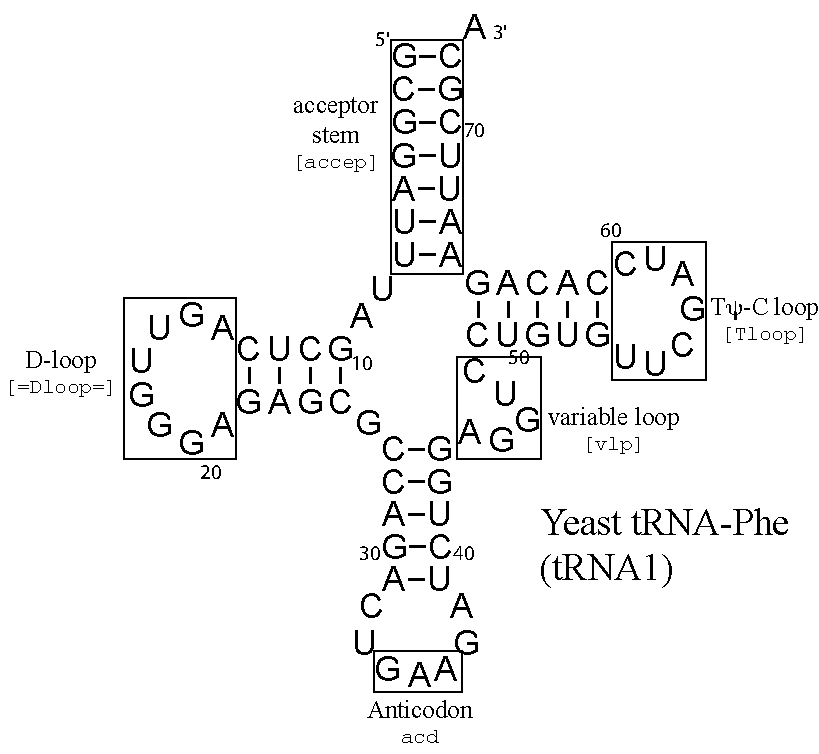
\includegraphics[scale=0.4]{Figures/trna1-DF6280-hand}
\end{minipage}
\vspace{1em}

This file is the same as \otext{tutorial/tRNA5.sto} except for the two
additional lines beginning with \otext{\#=GC RF}. This RF (reference)
annotation is required for using \otext{--hand}. When \otext{--hand}
is used, any non-gap character in the reference annotation will be
assigned as a match (consensus) position. Importantly, four different
characters are considered gaps: dashes (\otext{-}), underscores
(\otext{\_}), dots (\otext{.}) and tildes (\verb+~+). In this example
alignment, all columns are non-gap characters, so all columns will be
considered match positions.

Different regions of the secondary structure have been marked up using
abbreviations for the names of the regions in the reference
annotation. For example, \otext{acd} annotates the three positions of
the anticodon, and \otext{[vlp]} annotates the so-called variable
loop. I've used \otext{[} and \otext{]} to indicate region boundaries
in some cases. Crucially, I've avoided the use of any gap characters
for positions between named regions which I still want to be
considered match positions, and opted to use \otext{=} (which is not
considered a gap by \prog{cmbuild}) for these positions.

To build the hand-specified model from this alignment, do:

\user{cmbuild --hand tRNA5-hand.cm tutorial/tRNA5-hand.sto}
%tutorial regression: trna-hand-build.out

\begin{sreoutput}
# cmbuild :: covariance model construction from multiple sequence alignments
# INFERNAL 1.1.1 (July 2014)
# Copyright (C) 2014 Howard Hughes Medical Institute.
# Freely distributed under the GNU General Public License (GPLv3).
# - - - - - - - - - - - - - - - - - - - - - - - - - - - - - - - - - - - -
# CM file:                                            tRNA5-hand.cm
# alignment file:                                     ../../tutorial/tRNA5-hand.sto
# use #=GC RF annotation to define consensus columns: yes
# - - - - - - - - - - - - - - - - - - - - - - - - - - - - - - - - - - - -
#                                                                      rel entropy
#                                                                      -----------
# idx    name                     nseq eff_nseq   alen  clen  bps bifs    CM   HMM description
# ------ -------------------- -------- -------- ------ ----- ---- ---- ----- ----- -----------
       1 tRNA5-hand                  5     3.59     74    74   21    2 0.763 0.476 
#
# CPU time: 0.59u 0.00s 00:00:00.59 Elapsed: 00:00:00.61
\end{sreoutput}

The output reports that the model now has 74 match (consensus)
positions in the \otext{clen} column. If we had built this model
without specifying \otext{--hand} (as we did earlier in this tutorial)
the resulting model would have had only 72 consensus positions.
(I've annotated the two extra match positions with three gaps in
\otext{tRNA5.hand.sto} as match solely to demonstrate how
\otext{--hand} works, not because I think it's better to model these
positions as matches than inserts.)

Now, let's use this model to search the \emph{M. ruminantium} genome
again. First, the model must be calibrated. To save time, a calibrated
version of the file is in \otext{tutorial/tRNA5-hand.c.cm}. To do the
search:

\user{cmsearch tutorial/tRNA5-hand.c.cm tutorial/mrum-genome.fa}

The results are very similar to the earlier search with the
tRNA model built with default \prog{cmbuild} parameters (though not
identical since the model now has two additional match positions). The
important difference involves the hit alignments. Take a look at the
alignment for hit number 46 as an illustrative example:

\begin{widesreoutput}
>> NC_013790.1  Methanobrevibacter ruminantium M1 chromosome, complete genome
 rank     E-value  score  bias mdl mdl from   mdl to       seq from      seq to       acc trunc   gc
 ----   --------- ------ ----- --- -------- --------    ----------- -----------      ---- ----- ----
 (46) !   1.6e-09   43.2   0.0  cm        1       74 []      995344      995263 - .. 0.90    no 0.49

                                 v          v                                                            NC
                     (((((((,,<<<<________._>>>>,<<<<<_______>>>>>,,,........,,<<<<<_______>>>>>))))))): CS
   tRNA5-hand      1 gCcggcaUAGcgcAgUUGGuu.AgcgCgccagccUgucAagcuggAGg........UCCgggGUUCGAUUCcccGugccgGca 74    
                     :::G:CAUAGCG AG  GGU+ A CGCG:CAG:CU +++A:CUG: G+        UC:GGGGUUCGA UCCCC:UG:C:::A
  NC_013790.1 995344 AGAGACAUAGCGAAGC-GGUCaAACGCGGCAGACUCAAGAUCUGUUGAuuaguucuUCAGGGGUUCGAAUCCCCUUGUCUCUA 995263
                     ************9***.8886258***********************9444444445************************** PP
                     [accep]======[=Dloop=.]============acd=======[vl........p]=====[Tloop]=====[accep]= RF
\end{widesreoutput}

The reference annotation from the training alignment to \prog{cmbuild}
has been propagated to the hit as an extra \otext{RF} line at the
bottom of the alignment. All inserts in the alignment are annotated as
\otext{.} columns in the RF annotation. Note that the variable loop
(annotated as \otext{[vlp]} in the training alignment) contains 8
inserted residues. The RF annotation will also be transferred to
multiple alignments created with \prog{cmalign}.


\newpage
\section{Infernal 1.1's profile/sequence comparison pipeline}
\label{section:pipeline}
\setcounter{footnote}{0}

In this section, we briefly outline the processing pipeline for a
single profile/sequence comparison. This should help give you a sense
of what Infernal is doing under the hood, what sort of mistakes it may
make, and what the various results in the output actually mean. If you
haven't already worked through the tutorial section of the guide, you
should do that first before reading this section as it lays some
foundation for this discussion.

We'll first discuss the \emph{standard} pipeline used by Infernal,
which is excecuted on each comparison between a CM and full length
sequence. Then we'll discuss \emph{truncated variants} of the pipeline
that are \emph{re}run on the sequence ends for detection of truncated
hits. Finally, we'll cover the HMM-only pipeline which is run for
models with zero basepairs. Before we begin, a few notes on
terminology. In this discussion, the term ``profile'' refers to either
a profile HMM filter or a CM, and nucleotide and residue are used
interchangeably for a single symbol of an input DNA/RNA sequence (even
though ``residue'' traditionally refers to an amino acid residue of a
protein sequence). Also, if I refer to ``the pipeline'' without
specifying which variant (standard or a truncated one), then I mean
the standard one.

Infernal's standard pipeline is based closely on the profile
HMM/sequence comparison pipeline in HMMER3 (\url{hmmer.org}). In fact,
the first several stages of the pipeline use code from HMMER's
pipeline to score candidate sequences with profile HMMs that act as
filters for the later, more computationally expensive CM stages.

In briefest outline, the comparison pipeline takes the following
steps:

\begin{description}
\item[Profile HMM filter stages:] The first several stages of the
  pipeline use only a profile HMM, putting off all calculations with
  the CM until later. Since profile HMM algorithms are less complex
  than CM ones, this saves time by only using the expensive CM
  methods for regions the HMM has identified as having a good chance
  of containing a high-scoring hit. Of course, by relying on
  sequence-only based filters like HMMs, we are potentially going to
  miss homologs that are divergent at the sequence level but that the
  CM would still score highly thanks to conserved secondary
  structure. Our benchmarks reveal this is rare, but it does happen
  and is an important failure mode to keep in mind.

  The profile HMM filter stages are very closely based on the similar
  steps in HMMER3's accelerated comparison pipeline with the important
  difference that both \emph{local} and \emph{glocal} versions of HMM
  algorithms are used.

  Here's a list of the profile HMM filter stages:
\begin{description}
\item[\textbf{Null model.}] Calculate a score term for the ``null
  hypothesis'' (a probability model of \emph{non-}homology). This
  score correction is used to turn all subsequent profile/sequence bit
  scores into a final log-odds bit score.
  
\item[\textbf{Local scanning SSV filter.}] The SSV (``Single Segment
  Viterbi'') algorithm looks for high-scoring \emph{ungapped}
  alignments. Each sequence segment (referred to as a ``diagonal'') in
  a SSV alignment is extended slightly to define a window. Overlapping
  windows are merged together into a single window. Then, long windows
  greater than a maximum length $2L$ (where $L$ is the maximum of the
  model's $W$ parameter\footnote{$W$ is the expected maximum hit
  length for the model calculated by \prog{cmbuild} and stored in the
  CM file} and $1.25$ times the consensus length of the model) are
  split into multiple windows of length $2L$ with $L-1$ overlapping
  nucleotides between adjacent windows. Each window is then passed on
  to the next next pipeline step. Any nucleotides that are not
  contained in an SSV window are not evaluated further.

\item[\textbf{Local Viterbi filter.}] A more stringent accelerated
  filter. An optimal (maximum likelihood) gapped alignment score is
  calculated for each sequence window that survived SSV. If this score
  passes a set threshold, the sequence passes to the next step; else
  it is rejected.

\item[\textbf{Bias filter.}] A hack that reduces false positive
  Viterbi hits due to biased composition sequences. A two-state HMM is
  constructed from the mean nucleotide composition of the profile HMM
  and the standard nucleotide composition of the null model, and used
  to score the sequence window. The Viterbi bit score is corrected
  using this as a second null hypothesis. If the Viterbi score still
  passes the Viterbi threshold, the sequence passes on to the next
  step; else it is rejected. \emph{The bias filter score correction
  will also be applied to the local Forward filter and glocal Forward
  filter scores that follow.}
  
\item[\textbf{Local Forward filter.}] The full likelihood of
  the profile/sequence window comparison is evaluated, summed over the
  entire alignment ensemble, using the HMM Forward algorithm with the
  HMM in \emph{local} mode. This score is corrected to a bit score using the
  null model and bias filter scores. If the bit score passes a set
  threshold, the sequence window passes on to the next step; else it
  is rejected.

\item[\textbf{Glocal Forward filter/parser.}]  The HMM Forward
  algorithm is again used to evaluate the full likelihood of the
  profile/sequence window comparison, but this time the HMM is
  configured in \emph{global} mode, which requires that any valid
  alignment begin at the first consensus position (match or delete)
  and end at the final consensus position. (In local mode alignments
  can begin and end at any model positios.) Aligments in this stage,
  as in all previous stages can be local \emph{with respect to the
  sequence} (starting and ending at any sequence position), which is
  why this stage is referred to as \emph{glocal}: global with respect
  to the model and local with respect to the sequence. The glocal
  Forward score is corrected to a bit score using the null model and
  bias filter scores. If the bit score passes a set threshold, the
  sequence window passes on to the next step; else it is rejected.
  
\item[\textbf{Glocal envelope definition.}] Using the glocal Forward
  parser results, now combined with glocal Backward parser results,
  posterior probabilities that each nucleotide in the window is aligned
  to a position of the model are calculated. A discrete set of
  putative alignments is identified by applying heuristics to
  posterior probabilities. This procedure identifies \emph{envelopes}:
  subsequences in the target sequence window which contain a lot of
  probability mass for a match to the profile. The envelopes are often
  significantly shorter than the full window, containing only nucleotides
  that have a signficant probability of aligning to the HMM, which is
  critical for the subsequent CM stages of the pipeline. Each
  envelope's (there can be more than one if the evaluation reveals
  multiple full length alignments in a single window) glocal Forward
  score is corrected to a bit score using the null model and bias
  filter scores. If the bit score passes a set threshold, the sequence
  envelope passes on to the next step; else it is rejected.

\end{description}

\item[Covariance model stages:] The remainder of the pipeline uses the
  CM to evaluate each envelope that survived the profile HMM filter
  stages. 

\begin{description}
\item[\textbf{HMM banded CYK filter.}] For each envelope, posterior
  probabilities that each sequence residue aligns to each state of a
  profile HMM is computed\footnote{The profile HMM used at this stage
  is referred to as a CM plan 9 (CP9) HMM in it the code. It is
  similar but not identical to the one used for filtering. It was
  constructed to be maximally similar to the CM and includes
  transitions between insert and delete states not allowed in the
  HMMER plan 7 models used in the filtering steps. CP9 HMMs are
  essentially a reimplementation of the maximum likelihood heuristic
  HMM described in \citep{WeinbergRuzzo06}.} and used to derive bands
  (constraints) for the CM CYK algorithm \citep{Brown00,
  Nawrocki09b}. A banded version of the CYK algorithm is used to
  determine the bit score of the maximum likelihood alignment of any
  subsequence within the envelope to the CM that is consistent with
  the HMM-derived bands. If this score passes a set threshold, the
  sequence envelope passes on to the next step; else it is rejected. 
  Additionally, the boundaries of the envelope may be modified
  (shortened: the start position increased and/or the end position
  decreased) at this stage, as detailed below.

\item[\textbf{HMM banded Inside parser.}] The full likelihood of the
  profile/sequence envelope is now evaluated, summed over the entire
  alignment ensemble for every subsequence of the envelope, using the
  CM Inside algorithm. Again HMM bands are used to constrain the CM
  dynamic programming calculations. This procedure identifies zero or
  more non-overlapping \emph{hits}, each defined as a subsequence in
  the envelope. An \emph{ad hoc} ``null3'' hypothesis is constructed
  for each hit's composition and used to calculate a biased
  composition score correction. The null3 score is subtracted from the
  Inside bit score and an E-value is computed for that score.

\item[\textbf{CM bias filter: the ``null3'' model.}]  To reduce false
  positive CM hits due to biased composition sequences, the Inside
  score is adjusted using a bias filter that is similar, but not
  identical, to the one used by the HMM stages. A single state HMM is
  constructed with emission probabilities equal to the mean nucleotide
  composition of the sequence of the hit, and used to score the hit.
  The Inside bit score is corrected using this as a second null
  hypothesis.

\item[\textbf{Alignment.}] For each identified hit, the HMM banded
  Inside/Outside algorithm is performed and an optimal accuracy (also
  sometimes called maximum expected accuracy) alignment is
  calculated. 

\item[\textbf{Storage.}] Now we have a \emph{hit score} (and E-value)
  and each hit has an optimal accuracy alignment annotated with
  per-residue posterior probabilities.

\end{description}
\end{description}

\subsection{Filter thresholds are dependent on database size}
Before we go into more detail on each stage, we'll briefly discuss the
filter thresholds used for each stage of the pipeline. These are the
P-values required for a window or envelope to pass each stage of the
pipeline. Unlike in HMMER, in which the filter thresholds are always
the same regardless of the query and target, in Infernal, the HMM
filter thresholds are dependent on the size of the search space. We
use the parameter $Z$ in the code and in this documentation to
represent the search space.

For \prog{cmsearch}, $Z$ is the size of the target sequence database,
in total number of nucleotides, multiplied by 2 because both strands
of each sequence will be searched. For \prog{cmscan}, $Z$ is defined
differently; it is the length of the current query sequence (again,
multiplied by 2) in nucleotides \emph{multiplied by the number of
models in the target CM database}. 

In general, the larger the search space, the stricter the filter
thresholds become. The specific thresholds used for all stages of the
pipeline for all possible search space sizes $Z$ are given in
Table~\ref{tbl:thresholds}.

The rationale for making filter thresholds more strict as $Z$
increases is as follows. As $Z$ increases so too does the CM bit score
necessary for a hit to reach the E-value reporting threshold (by
default 10.0). If we assume that a hit's filter HMM score increases
1qwith its CM score (which should be true for most true homologs), then it
follows that we should be able to decrease filter P-value thresholds
as $Z$ increases without sacrificing sensitivity relative to an
unfiltered search. Of course, it's unclear exactly how much we can
decrease the thresholds by before we start losing an unacceptable
amount of sensitivity. We've taken an empirical approach to determine
this by measuring performance on an internal benchmark of remote
structural RNA homology search based on Rfam. The sets of filter
thresholds in Table~\ref{tbl:thresholds} were determined to achieve
what we feel is a good trade-off between sensitivity, specificity and
speed on that benchmark.

% Source of table:
% ~nawrockie/notebook/12_0326_talk_xfam/latex/xfam.tex
% 'Avg relative speed' row calc'ed using relative rmark3 times
% from 'Avg model per Gb time' row of the version of the
% table in ~nawrockie/notebook/12_0326_talk_xfam/latex/xfam.tex,
% and rounding.
%
\begin{center}
\begin{table}
\small
\begin{tabular}{lll|r|r|r|r|r|r|}
\multicolumn{3}{c}{} & \multicolumn{6}{|c|}{size of search space ($Z$)} \\ \cline{4-9}
               &      & model         &         & 2Mb     & 20Mb     & 200Mb  & 2Gb     &          \\
filter stage  & model & configuration & $<$ 2Mb & to 20Mb & to 200Mb & to 2Gb & to 20Gb & $>$ 20Gb \\  \hline
& & & & & & & & \\
SSV                 & HMM & local  & 0.35  & 0.35 & 0.35 & 0.15 & 0.15 & 0.06 \\
& & & & & & & & \\
Viterbi             & HMM & local  & off   & off & 0.15 & 0.15 & 0.15 & 0.02 \\
& & & & & & & & \\
Forward             & HMM & local  & 0.02  & 0.005 & 0.003 & 0.0008 & 0.0002 & 0.0002 \\
& & & & & & & & \\
Forward             & HMM & global & 0.02  & 0.005 & 0.003 & 0.0008 & 0.0002 & 0.0002 \\
& & & & & & & & \\
envelope definition & HMM & global & 0.02  & 0.005 & 0.003 & 0.0008 & 0.0002 & 0.0002 \\
& & & & & & & & \\
HMM banded CYK      & CM  & local  & 0.0001  & 0.0001  & 0.0001 & 0.0001 & 0.0001 & 0.0001 \\
& & & & & & & & \\
HMM banded Inside   & CM  & local  & E $\leq$ 10 & E $\leq$ 10 & E $\leq$ 10 & E $\leq$ 10 & E $\leq$ 10 & E $\leq$ 10 \\ \hline
& & & & & & & & \\
%Avg model per Gb time   & & 3.48h & 1.25h & 0.54h & 0.27h & 0.18h & 0.11h \\
\multicolumn{3}{c|}{Average relative running time per Mb} & 30.0 & 10.0 & 5.0 & 2.5 & 1.5 & 1.0 \\
\end{tabular}
\caption{\textbf{Default P-value survival thresholds used for each
  filter stage for different search space sizes $Z$.} These values can
  be changed with command-line options as described in the text. The
  ``HMM banded Inside'' stage is not actually a filter, hits with an
  E-value $\leq$ 10 after this stage are reported to the search output. 
  filter stage. The final line ``Average relative running time''
  provides rough estimates of the relative speed per Mb of the different
  parameter settings for each range of $Z$ (these are relative units,
  not an actual unit of time like minutes). Importantly, $Z$ is
  defined differently in \prog{cmsearch} and \prog{cmscan}. In
  \prog{cmsearch}, $Z$ is the total number of nucleotides in the
  target database file multiplied by 2 (because both strands of each
  sequence is searched). For \prog{cmscan}, $Z$ is the length of the
  current query sequence multiplied 2 (because both strands of the
  sequence are searched) and multiplied again by the number of CMs in
  the target CM database.}
\label{tbl:thresholds}
\end{table}
\end{center}

\subsection{Manually setting filter thresholds}

As described above, by default filter thresholds are automatically set
based on the search space $Z$, but several options exist for
overriding these defaults. There are four pre-defined sets of
thresholds, each available via a single command-line option to
\prog{cmsearch} or \prog{cmscan}. In order from least strict to most
strict these are: \ccode{--max}, \ccode{--nohmm}, \ccode{--mid}, and
\ccode{--rfam}. (The default thresholds lie somewhere between
\ccode{--mid} and \ccode{--rfam}.) Additionally, you can specify that
the filter thresholds be set as if the search space was \ccode{<x>}
megabases with the \ccode{--FZ <x>} option. More detail on each of
these options is provided below. A one-line description of each option
is printed as part of the \prog{cmsearch} and \prog{cmscan} 'help'
output that gets displayed with the use of the \ccode{-h}
option. There's also descriptions of these options in the
\prog{cmsearch} and \prog{cmscan} manual pages.

\begin{description}
\item[\ccode{--max}:] Turn off all filters, run Inside on full length
  target sequences. This option will result in maximum sensitivity but
  is also the slowest. Using this option will slow down
  \prog{cmsearch} by about 3 or 4 orders of magnitude for typical
  searches.
\item[\ccode{--nohmm}:] Turn off all profile HMM filters, run only the
  CYK filter on full length sequences and Inside on surviving
  envelopes. Searches with this option will often be between 5 and
  10 times faster than \ccode{--max} searches.
\item[\ccode{--mid}:] Turn off the SSV and Viterbi filters, and set
  all profile HMM filter thresholds (local Forward, glocal Forward and
  glocal domain definition) to the same, set P-value. By default this
  P-value is $0.02$, but it is settable to \ccode{<x>} by also using
  the \ccode{--Fmid <x>} option. 
\item[\ccode{--rfam}:] Set all filter thresholds as if the search
  space were more than 20 Gb. These are the filter thresholds used by
  a database like Rfam, which annotates RNAs in an EMBL-based sequence
  dataset that is several hundred Gb. If you're trying to
  reproduce results in future versions of Rfam that use Infernal 1.1
  (of course, at the time of writing, no version of Rfam yet exists
  which has used version 1.1) you probably want to use this option.
  This option will have no effect if the target search space is more
  than 20 Gb. 
\item[\ccode{--FZ <x>}:] Set the filter thresholds as if the search space
  were \ccode{<x>} Mb instead of its actual size. Importantly, the E-values
  reported will still correspond to the actual size. (To change the
  search space size the E-values correspond to, use the \ccode{-Z <x2>}
  option\footnote{Note that if you use \ccode{-Z <x2>} without
  \ccode{--FZ <x>}, the filter thresholds will be set as if the
  search space size is \ccode{<x2>} Mb.}.)
\end{description}

For expert users, options also exist to precisely set each individual
filter stage's threshold. Each stage is referred to by an option that
begins with \ccode{F} and ends with a number for the stages position
in the pipeline (SSV is F1, local Viterbi is F2, and so on). Also,
options that pertain to the bias filter part of each stage end in
\ccode{b}. The complete list of options for controlling the filter
thresholds is: \ccode{--F1}, \ccode{--F1b}, \ccode{--F2},
\ccode{--F2b}, \ccode{--F3}, \ccode{--F3b}, \ccode{--F4},
\ccode{--F4b}, \ccode{--F5}, \ccode{--F5b}, and
\ccode{--F6}. Additional options exist for turning on or of each stage
as well: \ccode{--noF1}, \ccode{--doF1b}, \ccode{--noF2},
\ccode{--noF2b}, \ccode{--noF3}, \ccode{--noF3b}, \ccode{--noF4},
\ccode{--noF4b}, \ccode{--noF5}, \ccode{--noF5b}, and \ccode{--noF6}.
Because these options are only expected to be useful to a small
minority of users, they are only displayed in the help message for
\prog{cmsearch} or \prog{cmscan} if the special \ccode{--devhelp}
option is used.

\subsection{In more detail: profile HMM filter stages}

Now we'll go back and revisit each stage of the pipeline in a bit more detail.

\subsubsection{Null model.}

The ``null model'' calculates the probability that the target
subsequence (window or envelope) is \emph{not} homologous to the query
profile. A profile HMM or CM bit score is the log of the ratio of the
sequence's probability according to the profile (the homology
hypothesis) over the null model probability (the non-homology
hypothesis).

The null model is a one-state HMM configured to generate ``random''
sequences of the same mean length $L$ as the target subsequence window
or envelope being evaluated\footnote{For the SSV filter, which
examines full length target sequences instead of windows, $L$ is set
as the expected maximum length of a hit for the profile, defined as
the maximum of the $1.25$ times the consensus length of the model and
the $W$ parameter for the CM we're filtering for. The $W$ parameter is
calculated by \prog{cmbuild}.}, with each residue drawn from a
background frequency distribution of $0.25$ for all four RNA
nucleotides (a standard i.i.d. model: residues are treated as
independent and identically distributed). This null model is used for
the profile HMM and the CM stages of the pipeline.

For technical reasons, the \emph{residue emission} probabilities of
the null model are incorporated directly into the profile HMM, by
turning each emission probability in the profile into an odds
ratio. The null model score calculation therefore is only concerned
with accounting for the remaining \emph{transition} probabilities of
the null model and toting them up into a bit score correction.  The
null model calculation is fast, because it only depends on the length
of the target sequence window being evaluated, not its sequence.

\subsubsection{SSV filter.}

The sequence is aligned to the profile using a specialized model that
allows a single high-scoring local ungapped segment to match.  The
optimal alignment score (Viterbi score) is calculated under this
specialized model, hence the term SSV, for ``single-segment
Viterbi''. SSV is similar, but not identical to, the MSV
(``multi-segment Viterbi) algorithm used by the programs in HMMER 
for protein sequence analysis. There are two main differences. First,
SSV only allows a single ungapped segment match between the sequence
and specialized model. Second, the variant of SSV used by Infernal is
designed for scanning along potentially long sequences (think
chromosomes instead of protein sequences) and potentially finding many
high-scoring hits in each sequence. This scanning SSV algorithm was
developed by Travis Wheeler for a soon-to-be released version of HMMER
that includes a program for DNA homology search called \prog{nhmmer}.

Vector parallelization methods are used to accelerate optimal ungapped
alignment in SSV. The P-value threshold for what subsequences pass
this filter range from $0.35$ for small target databases down to
$0.06$ for large ones (Table~\ref{tbl:thresholds}). Take as an
example, the \prog{cmsearch} for tRNAs performed in the tutorial. The
database size was roughly 6 Mb, so the SSV threshold was set as
$0.35$. This means that about 35\% of nonhomologous sequence is
expected to pass.

The SSV bit score is calculated as a log-odds score using the null
model for comparison. No correction for a biased composition or
repetitive sequence is done at this stage. For comparisons involving
biased sequences and/or profiles, more than 35\% of comparisons will
pass the SSV filter. For the tRNA search from the tutorial, the end of
the search output contained a line like:

\begin{sreoutput}
Windows   passing  local HMM SSV           filter:           11197  (0.2108); expected (0.35)
\end{sreoutput}

which tells you how many windows and what fraction of the total
database was comprised by those windows passed the 
SSV filter, versus what fraction was expected.

The \ccode{--F1 <x>} expert option sets filter P-value threshold for
passing the SSV filter to \ccode{<x>}. The \ccode{--doF1b} and
\ccode{--F1b <x>} options turn on a SSV bias filter (described further
below) and control its P-value threshold, respectively. SSV is turned
off if the \ccode{--max}, \ccode{--nohmm}, \ccode{--mid}, or
\ccode{--noF1} options are used.

\subsubsection{Local Viterbi filter.}
Each sequence window that survives the SSV filter is now aligned to
the profile HMM using a fast Viterbi algorithm for optimal gapped
alignment. This stage is identical the Viterbi stage of the HMMER3
pipeline. 

This Viterbi implementation is specialized for speed.  It is
implemented in 8-way parallel SIMD vector instructions, using reduced
precision scores that have been scaled to 16-bit integers. Only one
row of the dynamic programming matrix is stored, so the routine only
recovers the score, not the optimal alignment itself. The reduced
representation has limited range; local alignment scores will not
underflow, but high scoring comparisons can overflow and return
infinity, in which case they automatically pass the filter.

The final Viterbi filter bit score is then computed using the null
model score. 

As with SSV, and all other HMM filter stages, the local Viterbi filter
threshold depends on the search space $Z$. It is the only stage that
is actually turned off if $Z$ is low enough (less than $20$ Mb). 
For the tRNA search used in the tutorial $Z$ was less than $20$ Mb, so
the local Viterbi filter was turned off, and the following line was
included in the output in the pipeline summary output:

\begin{sreoutput}
Windows   passing  local HMM Viterbi       filter:                  (off)
\end{sreoutput}

For searches with $Z$ greater than $20$ Mb, this line would be
formatted similar to the one for the SSV filter. For example,
a search of the tRNA model from the tutorial against the
\emph{Saccharomyces cerevisiae} genome results in:

\begin{sreoutput}
Windows   passing  local HMM Viterbi       filter:           20666  (0.09861); expected (0.15)
\end{sreoutput}

In this search $20666$ windows have survived the local Viterbi filter,
comprising $0.09861$ fraction of all nucleotides searched. The
expected survival fraction was $0.15$. This large of a deviation from
expectation is common. One reason for it is that the $0.15$
expectation assumes that the full (100\%) of the database is subjected
to the Viterbi filter, but remember that only the fraction that
survived SSV will be (roughly 35\%). You might expect that in general
most of the windows that would eventually survive Viterbi would also
survive SSV, but surely some of them will fail to pass SSV which will
lower the expectation from $0.15$. Exactly how much it will lower it
is based on many factors and is probably difficult to predict
accurately - Infernal doesn't even try. So while $0.15$ is printed as
the expectation, you will often observe survival fractions
substantially lower than this. This same logic applies to all
downstream filter stages. There are other factors at play here too,
including biased composition effects, which will also impact the
accuracy of the survival fraction predictions of all other stages of
the pipeline.

The \ccode{--F2 <x>} option controls the P-value threshold for passing
the Viterbi filter, and can be turned off with \ccode{--noF2}.  The
local Viterbi filter is also turned off if the \ccode{--max},
\ccode{--nohmm}, or \ccode{--mid} options are used.

\subsubsection{Biased composition filter.}

It's possible for profile HMMs and/or sequences to have biased nucleotide
compositions that result in ``significant'' log-odds bit scores not
because the profile matches the sequence particularly well, but
because the \emph{null model} matches the sequence particularly badly.

In a few cases, profiles and/or target sequences are sufficiently
biased that too many comparisons pass the local Viterbi or local
Forward stages of the filter pipeline, causing Infernal speed
performance to be severely degraded.  The treatment of biased
composition comparisons is a serious problem for the HMM
implementations in HMMER and Infernal. Solving it well will require
more research. As a stopgap solution to rescuing most of the speed
degradation while not sacrificing too much sensitivity, an \emph{ad
hoc} biased composition filtering step is applied to remove highly
biased comparisons.

On the fly, a two-state HMM is constructed. One state emits nucleotides
from the background frequency distribution (same as the null1 model),
and the other state emits nucleotides from the mean nucleotide composition
of the profile (i.e. the expected composition of sequences generated
by the core model, including match and insert states
[\ccode{hmmer/src/p7\_hmm.c:p7\_hmm\_SetComposition()}]). Thus if the profile is
highly biased (A-rich, for example), this composition bias will be captured
by this second state. This model's transitions are arbitrarily set
such that state 1 emits an expected length of the size of the current
window, and state
2 emits an expected length of M/8 at a time (for a profile HMM of
consensus length
M). An overall target sequence length distribution is set to a mean of
$L$, identical to the null1 model.

The sequence is then rescored using this ``bias filter model'' in
place of the null1 model, using the HMM Forward algorithm.  A new
local Viterbi bit score is obtained. If the P-value of this satisfies
the local Viterbi bias filter threshold, the sequence passes to the
next stage of the pipeline.

The bias filter score is used in an analogous way in the next two
stages of the pipeline: the local Forward and glocal Forward stages.
The biased composition filter step compromises a small amount of
sensitivity.  Though it is good to have it on by default, you may want
to shut it off if you know you will have no problem with biased
composition hits.

The default value used for the local Viterbi bias filter depends on
the search space size, $Z$. Like the local Viterbi filter it is turned
off by default if $Z$ is less than $20$ Mb. So it too was off in the
example tRNA search from the tutorial, and the summary line in the
output was:

\begin{sreoutput}
Windows   passing  local HMM Viterbi  bias filter:                  (off)
\end{sreoutput}

For searches with $Z$ greater than $20$ Mb, this line would be
formatted similar to the one for the SSV filter. For example,
a search of the tRNA model from the tutorial against the
\emph{Saccharomyces cerevisiae} genome results in:

\begin{sreoutput}
Windows   passing  local HMM Viterbi  bias filter:           20342  (0.09712); expected (0.15)
\end{sreoutput}

So $20342$ windows survive this stage, making up $0.09712$ fraction of
the total sequence space searched. A similar line is included above
for the (non-bias) local HMM Viterbi filter, indicating that $20666$
windows passed that stage, meaning that $324$ windows were removed by
the Viterbi bias filter. 

The \ccode{--F2b <x>} option controls the P-value threshold for
passing the local Viterbi bias filter stage.  The \ccode{--noF2b}
option turns off (bypasses) the local Viterbi biased composition
filter. With this option, the local Viterbi filter will still be used,
but its score is not recomputed using the bias composition model.  The
local Viterbi bias filter is also turned off if the \ccode{--max} or
\ccode{--nohmm} options are used.

\subsubsection{Local Forward filter.}

Each surviving window is now aligned to the profile HMM using the full
Forward algorithm with the model configured in local mode (allowing
alignments to begin and end at any position of the model), which
calculates the likelihood of the target sequence given the profile,
summed over the ensemble of all possible alignments. This step is
identical to the ``Forward filter/parser'' stage of the HMMER
pipeline.

This is a specialized time- and memory-efficient Forward
implementation called the ``Forward parser''. It is implemented in
4-way parallel SIMD vector instructions, in full precision (32-bit
floating point). 

The local Forward filter bit score is calculated by correcting this
score using the standard null model log likelihood. If the P-value of
this score passes the local Forward filter threshold then it passes to
the Forward bias filter and the score is recomputed using the biased
composition model. If the P-value of this score passes the Forward
bias filter threshold, then this window is pass onto the next stage of
the pipeline\footnote{You might wonder why the intial score with just
the null model is even computed if the bias adjusted score must also
pass the threshold for the window to survive. We do this solely for
more informative output - so we can report how many windows fail to
pass at each of these two stages independently, to potentially alert
users if a large number of windows are being thrown out by the bias
filter alone.}. 

The local Forward filter threshold used depends on
the search space $Z$ (Table~\ref{tbl:thresholds}). For the tRNA search
in the tutorial, $Z$ was about ~$6$ Mb and the threshold for the local
Forward stage and its bias filter were set as $0.005$. The summary
output contains two lines of output pertaining to this stage:

\begin{sreoutput}
Windows   passing  local HMM Forward       filter:             140  (0.002747); expected (0.005)
Windows   passing  local HMM Forward  bias filter:             139  (0.002728); expected (0.005)
\end{sreoutput}

For this search $140$ windows survived the local HMM Forward filter,
and one of these was removed by the subsequent bias filter. 

The \ccode{--F3 <x>} and \ccode{--F3b <x>} control the P-value thresholds for
passing the local Forward and local Forward bias filter stages.  The
\ccode{--noF3} and \ccode{--noF3b} options turn off (bypasses) the
stages. Both filters are also turned off if the \ccode{--max} or
\ccode{--nohmm} options are used.

\subsubsection{Glocal Forward filter.}

Each surviving window is now aligned to the profile HMM again using the full
Forward algorithm, but this time with the model configured in global
mode, only allowing alignments that begin at the first position of the
model and end at the final position. This stage is referred to as
\emph{glocal} because it is global with respect to the profile HMM,
but (potentially) local with respect to the sequence window,
alignments can begin and end at any position in the sequence
window. 

For technical reasons related to the inability to guarantee a lower
bound on the glocal Forward score, glocal Forward is not implemented
with parallel SIMD vector instructions, and consequently it is
significantly slower than the local Forward filter
implementation. However, in practice it is run on a significantly
smaller fraction of the database than is the local stage, which
decreases the impact of this slower speed on the overall running time
of the search. 

It is not immediately obvious that using a glocal HMM filter stage is
a good idea, when our final CM stages of the pipeline will allow local
hits to the model. You might imagine that the glocal filter will
remove some windows that don't match well enough to the \emph{full}
model to survive but do contain a high-scoring local CM hit. This is
undoubtedly true in some cases (indeed, we could certainly construct
examples of this) but it does not seem to be common enough to be a
concern, at least based on our internal benchmarking. That is, using
both a local and glocal Forward filter does not seem to decrease
sensitivity compared with only using a local one. The reason probably
lies in the relatively high ($0.005$) filter threshold used at this
stage. Even hits that will eventually be reported as local hits still
contain surrounding sequence similar enough to the profile to make up
a global score that passes threshold.

An obvious failure mode of the glocal filter is for identifying 
hits that are truncated at one or both ends due to the beginning or
termination of a sequencing read. However, Infernal uses a special
pipeline for identifying these hits at the ends of sequences, as
described in a later section, so if they're missed at this stage, they
should be detected later when the truncated variants of the
pipeline are run.

The glocal Forward filter bit score is calculated by correcting the
score found by the Forward algorithm using the standard null model log
likelihood. If the P-value of this score passes the glocal Forward
filter threshold then it passes to the glocal Forward bias filter and the
score is recomputed using the biased composition model. If the P-value
of this score passes the glocal Forward bias filter threshold, then this
window is pass onto the next stage of the pipeline.

The glocal Forward filter threshold used depends on
the search space $Z$ (Table~\ref{tbl:thresholds}). For the tRNA search
in the tutorial, $Z$ was about ~$6$ Mb and the threshold for the glocal
Forward stage and its bias filter were set as $0.005$. The summary
output contains two lines of output pertaining to this stage:

\begin{sreoutput}
Windows   passing glocal HMM Forward       filter:              88  (0.001973); expected (0.005)
Windows   passing glocal HMM Forward  bias filter:              88  (0.001973); expected (0.005)
\end{sreoutput}

For this search $88$ of the $139$ windows evaluated by the glocal HMM
Forward filter survived, and none of them were removed by the subsequent bias filter. 

The \ccode{--F4 <x>} and \ccode{--F4b <x>} control the P-value thresholds for
passing the glocal Forward and glocal Forward bias filter stages.  The
\ccode{--noF4} and \ccode{--noF4b} options turn off (bypasses) the
stages. Both filters are also turned off if the \ccode{--max} or
\ccode{--nohmm} options are used.

\subsubsection{Envelope definition.}

A target sequence window that reaches this point is likely to be
larger than the eventual hit or hit(s) (if any) contained within it,
including nonhomologous nucleotides at the ends of the target sequence
window and possibly in between hits (if there are more than one). At
this stage, each window is transformed into one or more envelopes that
usually are significantly shorter than the original window. 

%Removing nucleotides that are not involved in an eventual hit
%non-homologous at this stage is crucial for the efficiency of the
%downstream CM stages of the pipeline which rely on sequence-based
%constraints which are tighter if only homologous sequence

Infernal's HMM envelope definition step is very similar to the
\emph{domain} definition step of HMMER, with the important difference
that the profile HMM is configured for global alignment instead of
local alignment.  The envelope definition step is essentially its own
pipeline, with steps as follows:

\paragraph{Backward parser.}
The counterpart of the glocal Forward filter algorithm is calculated.
The Forward algorithm gives the likelihood of all \emph{prefixes} of
the target sequence, summed over their alignment ensemble, and the
Backward algorithm gives the likelihood of all \emph{suffixes}. For
any given point of a possible model state/residue alignment, the
product of the Forward and Backward likelihoods gives the likelihood
of the entire alignment ensemble conditional on using that particular
alignment point. Thus, we can calculate things like the posterior
probability that an alignment starts or ends at a given position in
the target sequence.

\paragraph{Decoding.}
The posterior decoding algorithm is applied, to calculate the
posterior probability of alignment starts and ends (profile B and E
state alignments) with respect to target sequence position.

The sum of the posterior probabilities of alignment starts (B states)
over the entire target sequence window is the \emph{expected number of
hits} in the sequence window.

\paragraph{Region identification.}

A heuristic is now applied to identify a \emph{non-overlapping} set of
``regions'' that contain significant probability mass suggesting the
presence of a match (alignment) to the profile.

For each region, the expected number of envelopes is calculated (again
by posterior decoding on the Forward/Backward parser results). This
number should be about 1: we expect each region to contain one global
alignment to the profile. 

\paragraph{Envelope identification.}

Now, within each region, we will attempt to identify envelopes.
An envelope is a subsequence of the target sequence that
appears to contain alignment probability mass for a likely hit (one
global alignment to the profile).

When the region contains $\simeq$1 expected envelope, envelope
identification is already done: the region's start and end points are
converted directly to envelope coordinates.

In some cases, the region appears to contain more than
one expected hit -- where more than one hit is closely spaced on
the target sequence and/or the domain scores are weak and the
probability masses are ill-resolved from each other. These
``multi-hit regions'', when they occur, are passed off to an even
more \emph{ad hoc} resolution algorithm called \emph{stochastic
  traceback clustering}. In stochastic traceback clustering, we sample
many alignments from the posterior alignment ensemble, cluster those
alignments according to their overlap in start/end coordinates, and
pick clusters that sum up to sufficiently high probability. Consensus
start and end points are chosen for each cluster of sampled
alignments. These start/end points define envelopes.

It's also possible (though rare) for stochastic clustering to identify
\emph{no} envelopes in the region.

During envelope identification, the Forward algorithm is used to score
each putative envelope, and the standard null model (not the bias one)
is used as a correction (using mean length $L$ equal to the envelope
length) and this score is checked to see if it is below a P-value
threshold. This threshold is $Z$-dependent
(Table~\ref{tbl:thresholds}. For the tRNA search in the tutorial, this
threshold is $0.005$. If the P-value is less than the threshold the
envelope has survived all HMM filter stages and is passed onto the CYK
stage of the filter pipeline. 

In the tRNA search example, the summary output line for the envelope
definition stage is shown below (the line for the previous filter stage is also
shown for comparison):

\begin{sreoutput}
Windows   passing glocal HMM Forward  bias filter:              88  (0.001973); expected (0.005)
Envelopes passing glocal HMM envelope defn filter:             101  (0.001358); expected (0.005)
\end{sreoutput}

Note that while only $88$ windows were passed into this stage,
comprising $0.001973$ fraction of the total database, $101$ envelopes
survived making up $0.001358$ fraction of the database survived. Some
windows have been transformed into multiple envelopes and in general
the surviving envelopes are significantly shorter than the input
windows. 

The \ccode{--F5 <x>} expert option sets the filter P-value threshold for
passing the envelope definition filter to \ccode{<x>}. The \ccode{--doF5b} and
\ccode{--F5b <x>} options turn on a bias filter for this stage 
and control its P-value threshold, respectively. HMM envelope
definition is turned off if the \ccode{--max} or \ccode{--nohmm}
options are used.

\subsection{In more detail: CM stages of the pipeline}

After all profile HMM filter stages are complete, we have defined a
set of envelopes each of which may contain a single hit to the CM. We
now using sequence- and structure-based CM algorithms to score each
envelope and determine if it has a significant (reportable) hit to the
CM within it. Unfortunately, CM algorithms are computationally
expensive (more than an order of magnitude more complex than HMM
algorithms) so we need to constrain these algorithms in order to
incorporate them into a comparison pipeline that runs at a practical
speed. The acceleration technique used by Infernal relies on computing
and imposing bands on the CM dynamic programming matrices derived from
an HMM Forward/Backward decoding of the sequence, similar to the one
used in the envelope definition filter stage. This technique is based
on one pioneered by Michael Brown \citep{Brown00}. Next, we'll discuss the
calculation of those bands and how they're utilized to accelerate the
remaining CM stages of the pipeline.

\subsubsection{HMM band definition for CM stages.}

For each envelope that survives all the filter HMM stages,
sequence-specific bands are derived for a CYK dynamic programming
alignment of the envelope. The bands are derived from a HMM \\
Forward/Backward/Decoding steps (similar to those used in the envelope
definition pipeline) are used to determine the posterior probability
that each HMM position aligns to each sequence position of the
envelope. From these probabilities, \emph{bands} are determined for
each state, defined as sequence coordinate ranges that exclude only a
preset amount of the probability mass for that state. By default, the
excluded probability mass (referred to as tau ($\tau$) in the code) is
$0.0001$ ($1e-4$). For example, a band for state $x$ defined as
positions $10$ to $20$ (inclusive) of an envelope of length $30$
indicates that the summed probability of state $x$ aligning to
positions $1$ through $9$ and $21$ through $30$ is less than
$1e-4$. These HMM bands are then mapped onto the CM by converting them
to/from analogous states in the HMM and CM that model the same
position in the consensus model. A more detailed discussion of the
calculation and mapping of these bands can be found in
\citep{Nawrocki09b}.

The HMM used for deriving these bands is not the same one used in the
filter HMM stages of the pipeline. The new HMM used here is called a
CM Plan 9 (CP9) HMM, and it is constructed to be maximally similar to
a CM. These HMMs are essentially a reimplementation of of the maximum
likelihood heuristic HMM described in \citep{WeinbergRuzzo06}. 
CP9 HMMs are more similar to CMs than are the plan 7 HMMs of HMMER in
that they include transitions from delete states to insert states and
vice versa. These transitions are allowed in CMs, but not in plan 7
HMMs. Also, CP9 HMMs have special states for mirroring the local end
(EL) state of a CM, which don't occur in plan 7 HMMs.  Finally, these
CP9 HMMs are configured in a local mode with an uneven begin and end
probability distribution that places the highest probability on
beginning at model position 1 and ending at the final model position.
This local configuration more closely matches the CM local
configuration than both the local and global p7 filter HMM
configuration\footnote{In the plan 7 HMMER3 HMMs used in the filter
  stages, begin and end probabilities are equal for all positions of
  the model \citep{Eddy08}.}.

\subsubsection{HMM banded CM CYK filter.}

Given an envelope and CP9 HMM-derived bands constraining possible
alignments of a CM to the sequence positions in the envelope, a banded
version of the CM CYK algorithm is used to determine the
maximum-likelihood CM alignment\footnote{The CYK algorithm is the CM
analog of the HMM Viterbi algorithm.} of any subsequence in the
envelope to the CM that is consistent with the HMM bands \citep{Nawrocki09b}.

In most cases that occur in Infernal's pipeline, the HMM banded
version of CYK is significantly faster than non-banded, or even
query-dependent banded \citep{NawrockiEddy07} implementations of the CM
CYK algorithm. The speedup gained typically increases with the
consensus length of the model being used. However, HMM banded CYK is
only efficient when the target sequence alignment with an HMM is
well-resolved (includes at least some sequence position/model position
pairs that align with high probability), because only then will 
the resulting bands be ``tight'' and exclude a large fraction of
possible alignments. For this reason, the HMM filter stages of the
pipeline, in particular the envelope definition stage, are crucial for
enabling the HMM banded CM stages to work efficiently. 

The null-corrected CYK bit score (corrected using the same type of
equiprobable (25\% A, C, G and U) iid, null model used by the profile
HMM filter stages) is returned from the HMM banded CYK algorithm. No
bias correction is used at this stage. If this score has a P-value
less than $0.0001$ then the envelope is passed to the next stage of
the pipeline. Unlike in the HMM filter stages, the P-value threshold
used for the CYK filter is not dependent on the search space $Z$, but
it is controllable with the \ccode{--F6} option.

Envelope boundaries are potentially redefined at this stage based on
CYK scores. Envelopes can only be shortened, not extended, at either
boundary. We take advantage of the fact that the CYK algorithm
computes the maximum likelihood alignment score (consistent with the
HMM bands) of all possible subsequences in the envelope to the CM, and
examine each nucleotide to see if it is included in any possible
alignment to the model above a certain score threshold. By default,
this threshold is a 10-fold lower P-value than the filter survival
threshold, so it is $0.001$ ($10*0.0001$). This envelope redefinition
can be turned off with the \ccode{--nocykenvx} option and it the
threshold for it can be changed with the \ccode{--cykenvx <x>} option.

\subsubsection{HMM banded CM Inside filter/parser.}

Envelopes that survive CYK are evaluated using the CM Inside
algorithm, which is the CM analog of the HMM Forward algorithm. HMM
bands are rederived for this step (remember the envelope boundaries
may now be different), using a smaller $\tau$ value of $5e-6$. With
Inside, the probability of all possible alignments (instead of just
the most likely one) of each subsequence to the model that is
consistent with the bands are summed to define a probability for that
subsequence. A log-odds score is determined by applying two null
models: the standard null model used in CYK and an alternative null3
model based on the composition of the aligned subsequence. The null3
model is explained below.

A non-overlapping set of subsequence/model hits that fall below the
reporting E-value threshold is then collected using a greedy
approach\footnote{This greedy approach is as follows: while any hits
below threshold that do not overlap with previously reported ones
remain, select the top scoring one and report it}. Each hit is defined
by a start/end position in the envelope. 

By default, the reporting threshold is an E-value of $10.0$, but this
is settable to a different E-value with the \ccode{-E <x>} option, or
to a particular bit score with the \ccode{-T <x>} option.

\subsubsection{Optimal accuracy alignment.}

For each hit reported by Inside, an optimally accurate
alignment\footnote{This is the same type of alignment referred to as
``maximum expected accuracy'' in the HMMER documentation} is computed
using HMM banded versions of the Inside and Outside algorithm (using
the same bands from the Inside filter) and annotated with posterior
probabilities for each aligned nucleotide. The optimally accurate
alignment is the alignment that maximizes the sum of the posterior
probabilities of all aligned nucleotides. The alignment is then stored in
memory until the end of the search when it is finally output as part
of a ranked list of hits and their alignments.

\subsubsection{Biased composition CM score correction: the null3 model.}

CM Inside scores are adjusted using an alternative null hypothesis
called the null3 model in an effort to counteract the contribution of
biased sequence composition to the scores of hits. The null3 model
was motivated by the observation that many high-scoring false positive
hits in CM searches are to regions of the target database with with
highly biased residue composition, in particular regions with high
percentages of A and U residues.  If a model has a bias for a
particular residue, for example A, and a target region is composed of
an overrepresentation of that residue then it will receive a high
score simply because it is A-rich.

A different null3 model is calculated for every alignment. The 4
emission probabilities of the null3 model are calculated as 
simply their occurence within the region of the hit. For example, if
the hit is 50 residues long and contains $20$ As, $5$ Cs, $5$ Gs and $20$ Us,
then the null3 model probabilitiles will be calculated as $(0.4, 0.1,
0.1, 0.4)$. 

The null3 model is similar to the bias filter model used in the
profile HMM stages but it often gives more severe corrections for
highly biased hits because it is a single HMM state with emission
probabilities defined by the hit composition, not the model
composition. Importantly, scores collected during model calibration
for estimating E-value parameters in \prog{cmcalibrate} are also
corrected using the null3 model.

The null3 model is used in combination with the standard null model
(single state equiprobable A,C,G and U, same as the profile HMM
standard null model). We told you earlier that an Infernal bit score
is the log of the ratio of the sequence's probability according to the
profile over the null model probability, but how do we calculate this
score if we have more than one null hypothesis?  Infernal does a bit
of algebraic sleight of hand here, to arrive at an additive correction
to the original score that it calls the ``null3 score correction''.

\paragraph{Derivation of the null3 score correction}

We arrived at the parameters of the null3 model in a very \emph{ad
hoc} way. However, after that, the way Infernal arrives at the final bit
score once the null3 parameters have been determined is clean
(e.g. derivable) Bayesian probability theory. It is analagous to the
way HMMER uses the \emph{null2} score correction.

If we take the Bayesian view, we're interested in the probability of a
hypothesis $H$ given some observed data $D$:

\[
   P(H | D) = \frac{P(D | H) P(H)}{\sum_{H_i} P(D | H_i) P(H_i)},
\]

an equation which forces us to state explicit probabilistic models not
just for the hypothesis we want to test, but also for the alternative
hypotheses we want to test against. Up until now, we've considered two
hypotheses for an observed sequence $D$: either it came from our
CM (call that model $M$), or it came from our null hypothesis
for random, unrelated sequences (call that model $N$). If these are
the only two models we consider, the Bayesian posterior for the model
$M$ is:

\[
   P(M | D) = \frac{P(D | M) P(M)}{P(D | M) P(M) + P(D | N) P(N)}
\]

Recall that the log odds score (in units of bits) reported by
Infernal's alignment algorithms is

\[
  s = \log_2 \frac{P(D | M)}{P(D | N)}.
\]

Let's assume for simplicity that \emph{a priori}, the profile and the
null model are equiprobable, so the priors $P(M)$ and $P(N)$
cancel. Then the log odds score $s$ is related to the Bayesian
posterior by a sigmoid function,

\[
  P(M | D) = \frac{2^s}{2^s + 1}.
\]

(We don't have to assume that the two hypotheses are equiprobable;
keeping these around would just add an extra $\pi = \log P(M) / P(N)$
factor to $s$. We'll reintroduce these prior log odds scores $\pi$
shortly.)

The simple sigmoid relationship between the posterior and the log odds
score suggests a plausible basis for calculating a score that includes
contributions of more than one null hypothesis: \textbf{we desire a
generalized score $S$ such that:}

\[
  \frac{2^S}{2^S + 1} = P(M | D),
\]

\textbf{for \emph{any} number of alternative hypotheses under consideration.}

So, let $N_i$ represent any number of alternative null models
$N_i$. Then, by algebraic rearrangement of Bayes' theorem,

\[
   S = \log \frac{P(D | M) P(M)}{ \sum_{i} P(D | N_i) P(N_i)}. 
\]

We saw above that Infernal internally calculates a log odds score $s$, of
the model relative to the first null hypothesis. Let's now call that
$s_M$, the alignment score of the model. Infernal extends that same
scoring system to all additional competing hypotheses, calculating a
log odds score relative to the first null hypothesis for any
additional null hypotheses $i > 1$:

\[
  s_i = \log \frac{P(D | N_i)}{P(D | N_1)}
\]

We can also state prior scores $\pi_i$ for how relatively likely
each null hypothesis is, relative to the main one:

\[
  \pi_i = \log \frac{P(N_i)}{P(N_1)}
\]

(Remember that we assumed $\pi_M = 0$; but we're going to put it back
in anyway now.)

Now we can express $S$ in terms of the internal scores $s$ and
prior scores $\pi$:

\[
   S = \log  \frac{e^{s_M + \pi_M}} { 1 + \sum_{i>1} e^{s_i + \pi_i}},
\]

which therefore simply amounts to an additive correction of the
original score, $(s_M + \pi_M)$:

\[
  S = (s_M + \pi_M) - \log \left( 1 + \sum_{i>1} e^{s_i + \pi_i} \right)
\]

So, to calculate its reported score, Infernal uses four quantities:

\begin{enumerate}
\item [$s_M$] The (simple, uncorrected) log odds score for the model,
calculated by optimal alignment of the model to the sequence.

\item [$\pi_M$] The log odds of the priors, $\log P(M)/P(N_1)$. Infernal
   implicitly assumes this factor to be 0.

\item [$s_2$] The (simple, uncorrected) log odds score
   for the null3 hypothesis, calculated by rescoring the residues
   of the alignment under the null3 model.

\item [$\pi_2$] The log odds of the priors, $\log P(N_2)/P(N_1)$. 
Infernal arbitrarily assumes that the null3 model is
$\frac{1}{65536}$ as likely as the main null model, so this factor
is -16 bits.\footnote{In versions 1.0 through 1.0.2, the null3 model
  was assumed to be $\frac{1}{32}$ as likely as the main null model
  (-5 bit factor instead of -16 bits). The decreased value in version
  1.1 means that null3 penalties are reduced. We decided to do this
  based on internal benchmarking results. Version 1.1 uses a new
  default prior for parameterizing models which apparently alleviates
  the problem of biased composition, thus allowing us to reduce this
  value without sacrificing performance.}
\end{enumerate}

The code that calculates the null3 correction is in 
\prog{cm\_parsetree.c:ScoreCorrectionNull3()}.

The null3 correction is usually close to zero, for random sequences,
but becomes a significant quantitative penalty on biased composition
sequences.  It gets added to the original alignment score to form
Infernal's final bit score.

The null3 score correction is introduced in version 1.0 and was not
present in any of the 0.x versions of Infernal. This can
lead to large differences in the scores reported by 1.0 and previous
versions. 

The following table shows the penalty for a $100$ nucleotide hit with
varying compositions of A, C, G, and U residues. This table is included to give you
an idea of how severe the null3 correction is, and can be useful for
comparing bit scores from Infernal 1.0 to previous
versions (which did not use the null3 correction). These are just a
sample of the possible composition of hits you might see. Again, these
scores are for $100$ nucleotide hits, to determine the correction for
a hit of length $x$ simply multiply the corresponding correction below
by $x/100$. For example, a $35$\% A, $15$\% C, $15$\% G, $35$\% U hit
of length $100$ nt would receive a $6.88$ bit penalty from
null3 (row 4). A $200$ nt hit of the same composition would
receive a penalty of $13.76$ bits. A $50$ nt hit of the same
composition would receive a $3.44$ bit penalty.

\vspace{0.5in}

\begin{center}
\begin{tabular}{r|rrrr|c}
      &        &        &        &        & NULL3 \\ 
  GC\%&    A\% &   C\%  &   G\%  &    U\% & correction (bits)  \\ \hline
  0.0 &   50.0 &    0.0 &    0.0 &   50.0 &              95.00 \\
 10.0 &   45.0 &    5.0 &    5.0 &   45.0 &              48.10 \\
 20.0 &   40.0 &   10.0 &   10.0 &   40.0 &              22.81 \\
 30.0 &   35.0 &   15.0 &   15.0 &   35.0 &               6.88 \\
 35.0 &   32.5 &   17.5 &   17.5 &   32.5 &               2.01 \\
 40.0 &   30.0 &   20.0 &   20.0 &   30.0 &               0.30 \\
 45.0 &   27.5 &   22.5 &   22.5 &   27.5 &               0.07 \\
 50.0 &   25.0 &   25.0 &   25.0 &   25.0 &               0.04 \\
 55.0 &   22.5 &   27.5 &   27.5 &   22.5 &               0.07 \\
 60.0 &   20.0 &   30.0 &   30.0 &   20.0 &               0.30 \\
 65.0 &   17.5 &   32.5 &   32.5 &   17.5 &               2.01 \\
 70.0 &   15.0 &   35.0 &   35.0 &   15.0 &               6.88 \\
 80.0 &   10.0 &   40.0 &   40.0 &   10.0 &              22.81 \\
 90.0 &    5.0 &   45.0 &   45.0 &    5.0 &              48.10 \\
100.0 &    0.0 &   50.0 &   50.0 &    0.0 &              95.00 \\

\end{tabular}
\end{center}

\vspace{0.5in}

% obtained using esl-null3 a specialized easel miniapp
% created basically solely to make this table. 
% A frozen copy of the version used to make this table
% (with -l option)  
% is: /groups/eddy/home/nawrockie/notebook/12_0503_inf_tutorial/wd-infernal/easel/miniapps/bkups/12_0605-1/
%
% raw output:
% > esl-null3 -l 
%   GC      A      C      G      U  correction (bits)
%-----  -----  -----  -----  -----  -----------------
%100.0    0.0   50.0   50.0    0.0           84.00000
% 90.0    5.0   45.0   45.0    5.0           37.10043
% 80.0   10.0   40.0   40.0   10.0           11.80760
% 70.0   15.0   35.0   35.0   15.0            0.08019
% 65.0   17.5   32.5   32.5   17.5            0.00213
% 60.0   20.0   30.0   30.0   20.0            0.00016
% 55.0   22.5   27.5   27.5   22.5            0.00004
% 50.0   25.0   25.0   25.0   25.0            0.00002
% 45.0   27.5   22.5   22.5   27.5            0.00004
% 40.0   30.0   20.0   20.0   30.0            0.00016
% 35.0   32.5   17.5   17.5   32.5            0.00213
% 30.0   35.0   15.0   15.0   35.0            0.08019
% 20.0   40.0   10.0   10.0   40.0           11.80759
% 10.0   45.0    5.0    5.0   45.0           37.10044
%  0.0   50.0    0.0    0.0   50.0           84.00000

By default, the null3 score correction is used by \prog{cmcalibrate,
cmsearch} and \prog{cmscan}. It can be turned off in any of these
programs by using the \prog{--nonull3} option. However, be careful,
the E-values for models that are calibrated with \prog{--nonull3} are
only valid when \prog{--nonull3} is also used with \prog{cmsearch} or
\prog{cmscan}. Likewise, if \prog{--nonull3} is \emph{not} used during
calibration, it should not be used during searches or scans.

\subsection{Truncated hit detection using variants of the pipeline}

The Infernal pipeline discussed above is designed to find complete RNA
homologs within a (usually) larger sequence, e.g. a choromosome.
\emph{Final} hits may be local (not full-length) with respect to the
model, but the glocal HMM filter stage requires that at least some
statistical signal remain in a full length match to the profile
HMM. That is, enough signal to result in a good enough glocal Forward
score to pass the glocal filter (e.g. a P-value of $0.005$ for a
search space between 2 and 20 Mb). In our benchmarking, the vast
majority of statistically significant CM hits do pass the glocal
Forward HMM filter, however, there is the obvious failure mode of the
pipeline on \emph{truncated} hits. A truncated hit is defined as a hit
that is missing one or more nucleotides at the 5' and/or 3' end solely
because of the position where the sequencing read happened to begin or
end. While the chromosome the read derives from presumably included a
full length hit, the read itself does not because the sequencing
reaction used to determine the sequence began or ended at a position
internal to the hit. Infernal uses modified versions of its
profile/sequence comparison pipeline for detection of truncated hits.
This modified pipeline is executed after the full sequence is examined
with the standard pipeline.

The modified pipeline is only used near the sequence termini because
Infernal only expects truncated hits to occur due to the premature
ending of a sequencing read\footnote{There are cases where truncated
hits might occur within sequences (``split tRNAs'' in archaea
\citep{Randau05}, for example), but these are rare and Infernal does
not explicit look for these types of hits, unless the
\ccode{--anytrunc} option is used, as discussed at the end of this
section.}. Specifically only the first or final $X$ nucleotides at
either sequence end are examined for truncated hits, where $X$ is
defined as the minimum of the $W$ parameter (maximum expected hit
length, calculated in \prog{cmbuild}) and $1.25$ times the consensus
length of the model.

There are three variants of the pipeline used for truncated hit
detection:

\begin{enumerate}

\item \textbf{5' truncated hit detection.}
This pipeline is used only on the $X$ 5'-most nucleotides of each
sequence. These $X$ nucleotides are also searched along with the rest
of the complete sequence as part of the standard pipeline. Only 5'
truncated or non-truncated alignments can be found by this pipeline
variant, but non-truncated alignments will be duplicates of
those found previously by the standard pipeline. 

\item  \textbf{3' truncated hit detection.}
This pipeline is used only on the $X$ 3'-most nucleotides of each
sequence. These $X$ nucleotides are also searched along with the rest
of the complete sequence as part of the standard pipeline. Only 3'
truncated or non-truncated alignments can be found by this pipeline
variant, but non-truncated alignments will be duplicates of
those found previously by the standard pipeline. 

\item  \textbf{5' and 3' truncated hit detection.}
This pipeline is used only on complete sequences that are less than
$X$ nucleotides long. These sequences are also searched in their
entirety by the standard pipeline, the 5' truncated variant pipeline,
and the 3' truncated variant pipeline. Any types of alignments are
possible at this stage (5' truncated, 3' truncated, 5' \emph{and} 3'
truncated or non-truncated) but only 5' \emph{and} 3' truncated
alignments will not be duplicates of previously found alignments. 

\end{enumerate}

Given a sequence to search, the standard pipeline described in the
first part of this section is used on the full sequence. Then the
truncated pipeline variants 1 and 2 are used on the sequence
termini. Finally, if the sequence is less than $X$ nucleotides long,
variant 3 is used. Before hits are output, overlapping hits
potentially found in different variants of the pipeline are removed,
by keeping the highest scoring one. Also, remember that Infernal
searches both strands of each sequence, so each pipeline is run
separately on each strand.

It may seem like Infernal is duplicating effort by searching the first
and final $X$ nucleotides twice, i.e. once in the standard pipeline
and once in the 5' truncated variant or the 3' truncated variant. One
might argue that only searching these $X$ nucleotides with the
truncated pipeline variant should be sufficient to find truncated and
non-truncated hits. However, as we'll discuss next, the glocal HMM
filter stages, HMM band construction and the CYK and Inside algorithms
are different between the standard and truncated variants of the
pipeline and some non-truncated hits found by the standard variant
will be missed by the truncated variants, and vice versa. So it is
important we search the $X$ terminal nucleotides on the 5' and 3' end
using both standard and truncated variants of the pipeline. The same
is true of sequences that are less than $X$ nucleotides, which get
searched four times, once by each of the four pipeline variants (the
standard plus the three truncated variants).

\subsubsection{Differences between the standard pipeline and the
  truncated variants}

For all three truncated variants of the pipeline, the first three HMM
filter stages (SSV, local Viterbi and local Forward), as well as their
bias composition corrections, are identical to the standard pipeline
described above. However, the glocal HMM Forward, glocal HMM envelope
definition, CYK and Inside differ to accomodate truncated hits.

Recall that in the standard pipeline in the glocal HMM Forward and
envelope definition stages, the HMM is configured in global mode which
forces all alignments to begin in the first model position and end in
the final one (in the match or delete state in both cases). Also, in
these stages, the alignment could begin or end in any position of the
sequence window (i.e. local with respect to the sequence).  These
aspects of these two pipeline stages differ in the truncated variants.
For the 5' truncated pipeline variant, alignments can begin
at any model position but must end at the final model position,
\emph{and} the \emph{first} nucleotide in the window must be aligned to an HMM
model position. The 3' truncated pipeline variant does the opposite,
allowing alignments to end at any position but requiring they start at
the first position \emph{and} requiring that the \emph{final} nucleotide
in the sequence be aligned to an HMM model position. 
In the 5' and 3' truncated pipeline variant, alignments can begin and
end at any model position but the first and final nucleotide of the
sequence window must both be aligned to model positions. 

Similar changes are necessary for the truncated pipeline variants in
the CM pipeline stages. The HMM bands are computed using CP9 HMMs
configured in modified ways, similar to the modifications for the
filter HMMs in the glocal filter stages. Specifically, in the 5'
variant the first nucleotide in the window must be aligned to the
model and model \emph{begin} probabilities are equal for all model
positions. In the 3' variant, the final nucleotide in the window must
be aligned to the model and the model \emph{end} probabilities are
equal for all model positions. In the 5' and 3' variant, the first and
final nucleotides (i.e. all nucleotides) in the window must be aligned
to the model and model begin \emph{and} end probabilities are equal
for all model positions.

Also, additional score corrections are used in the CM stages to
compensate for the fact that alignments are now allowed to begin
and/or end at any model position to account for the truncation. The
correction is roughly the log of $1/M$ bits for the 5'-only and
3'-only pipeline variants, and roughly the log of $2/(M*(M+1))$ bits
for the 5' and 3' pipeline variant. For all hits found in a truncated
pipeline variant, this correction is subtracted from the CM bit score. 

For the CYK and Inside stages, specialized versions of the CM
alignment algorithms are necessary to cope with truncated
alignments. Allowing truncated alignments requires more changes to CM
algorithms than for HMM algorithms because CMs are arranged in a
tree-like structure instead of in a linear structure like HMMs, and
need to be able to deal with the possibility that the sequence
aligning to part of a subtree of the model has been truncated
away. For example, a truncated CM alignment algorithm must be able to
deal with the case where the left half but not the right half of a
stem has been deleted, and vice versa. For details on CM truncated
alignment, see \citep{KolbeEddy09}. HMM banded, truncated versions of
CYK and Inside are implemented in Infernal, and are used by the
truncated pipeline variants (see \ccode{src/cm\_dpsearch\_trunc.c} and
\ccode{src/cm\_dpalign\_trunc.c}. These implementations allow either 5'
truncation, 3' truncation, or both, and can require that valid
alignments begin at the first nucleotide of the sequence or end at the
final nucleotide of the sequence.  For the 5' truncated pipeline
variant, only 5' truncations are allowed and all valid alignments must
begin with the first nucleotide of the sequence. For the 3' variant,
only 3' truncations are allowed and all valid alignments must end with
the final nucleotide of the sequence. For the 5' and 3' pipeline
variant, 5' and/or 3' truncations are allowed, but all valid
alignments must include all nucleotides of the sequence.

%REF TO FIGURE WITH ALIGNMENT DISPLAY OF TRUNCATED HITS.

\subsubsection{Modifying how truncated hits are detected using
  command-line options}

The description above of the truncated variants of the pipeline
describe Infernal's default behavior. You can turn off truncated hit
detection with the \ccode{--notrunc} option. You can also modify how 
truncated hit detection works with the \ccode{--anytrunc} option. With
\ccode{--anytrunc}, truncated hits are allowed to occur anywhere
within a sequence, instead of necessarily including the first or final
nucleotide. 

Importantly, the truncated variants of the pipeline are currently not
implemented for use with non-HMM banded alignment. This means that the
they are incompatible with the \ccode{--max} options and
\ccode{--nohmm} options. When either of these options are used,
truncated hit detection is automatically turned off.

\subsection{HMM-only pipeline variant for models without structure}

As mentioned and demonstrated in the tutorial section of the guide,
Infernal uses a special HMM-only pipeline for models that have zero
basepairs. For a family with zero basepairs, it makes sense to use a
profile HMM instead of a covariance model because they will be very
similar models (the only important difference between CMs and profile
HMMs is the former's ability to model two basepaired positions as
dependent on one another) and HMM algorithms are more efficient than
CM ones. So a profile HMM search will be as sensitive but faster than
a CM one for families with zero basepairs.  When \prog{cmsearch} or
\prog{cmscan} is being used for a comparison between a sequence and a
model with zero basepairs, it will automatically use the HMM-only
filter pipeline. For these models, the truncated variants of the
pipeline are not used, because the standard HMM pipeline is capable of
identifying truncated hits.

The HMM-only pipeline that Infernal uses is essentially identical to
HMMER3's (version 3.0) pipeline, with the lone
difference that the scanning local SSV filter (described for the
standard pipeline above) replaces the full-sequence (non-scanning) MSV
filter used in HMMER. The scanning SSV filter was originally
implemented by Travis Wheeler for a new program in a
soon-to-be-released version of HMMER called \prog{nhmmer} for DNA
homology search.

We won't go through the HMM-only pipeline in as much detail as the
standard one (for more, see the HMMER3 user's guide
\citep{hmmer3guide}), but briefly the HMM-only pipeline consists of
the following steps: local scanning SSV filter to define windows, a
bias filter to correct SSV scores for biased composition (identical to
the one in the standard pipeline used after the local Viterbi stage),
local Viterbi filter for each window, and finally local Forward filter
for each window. Windows that survive the local Forward filter are
then subject to the 'domain identification' stage of the HMMER
pipeline, which identifies hits after full alignment ensemble
calculation using the Forward and Backward algorithms. Each hit is
then aligned to the HMM using an optimal accuracy alignment algorithm
that maximizes the summed posterior probability of all aligned
residues. The null3 biased composition model is not used in the
HMM-only pipeline, but HMMER's null2 biased composition model is used, 
see the HMMER3 guide for details on null2.

Unlike in the standard pipeline, the filter thresholds used in the
HMM-only pipeline are always the same, i.e. they are not dependent on
the size of the search space. The default thresholds are the same
values used in the HMMER3 pipeline: the SSV filter threshold is
$0.02$, the local Viterbi threshold is $0.001$ and the local Forward
threshold is $1e-5$. These can be changed with the \ccode{--hmmF1}
(SSV), \ccode{--hmmF2} (Viterbi) and \ccode{--hmmF3} (Forward). The
\ccode{--hmmmax} option runs the HMM-only pipeline in maximum
sensitivity mode with the SSV P-value threshold set at 0.3 and the
Viterbi and Forward filters turned off. The HMM-only pipeline can be
turned off with the \ccode{--nohmmonly} option. When turned off, all
models will use the standard and truncated CM pipelines, even those
with no structure.


\newpage
\section{Profile SCFG construction: the \texttt{cmbuild} program}

\software{infernal} builds a model of consensus RNA secondary
structure using a formalism called a \emph{covariance model} (CM),
which is a type of \emph{profile stochastic context-free grammar}
(profile SCFG) \cite{Eddy94,Durbin98,Eddy02b}.

What follows is a technical description of what a CM is, how it
corresponds to a known RNA secondary structure, and how it is built
and parameterized.\footnote{Much of this text is taken from
\cite{Eddy02b}.}  You certainly don't have to understand the technical
details of CMs to understand \prog{cmbuild} or \software{infernal},
but it will probably help to at least skim this part. After that is a
description of what the \prog{cmbuild} program does to build a CM from
an input RNA multiple alignment, and how to control the behavior of
the program.

\subsection{Technical description of a covariance model}

\subsubsection{Definition of a stochastic context free grammar}

A stochastic context free grammar (SCFG) consists of the following:

\begin{itemize}
\item $M$ different nonterminals (here called \emph{states}). I will use capital
      letters to refer to specific nonterminals; $V$ and $Y$ will be used
      to refer generically to unspecified nonterminals.
\item $K$ different terminal symbols (e.g. the observable alphabet,
      {a,c,g,u} for RNA). I will use small letters $a,b$ to refer
      generically to terminal symbols.
\item a number of \emph{production rules} of the form: $V \rightarrow
\gamma$, where $\gamma$ can be any string of nonterminal and/or
terminal symbols, including (as a special case) the empty string
$\epsilon$.
\item Each production rule is associated with a probability, such that
      the sum of the production probabilities for any given
      nonterminal $V$ is equal to 1.
\end{itemize} 

\subsubsection{SCFG productions allowed in CMs}

A CM is a specific, repetitive SCFG architecture consisting of groups
of model states that are associated with base pairs and
single-stranded positions in an RNA secondary structure consensus. A
CM has seven types of states and production rules:

\vspace{0.5em}
\begin{center}
\begin{tabular}{lllll}
State type & Description             &  Production             & Emission & Transition\\ \hline
P & (pair emitting)   & $P \rightarrow a Y b$ & $e_v(a,b)$ & $t_v(Y)$  \\
L & (left emitting)   & $L \rightarrow a Y$   & $e_v(a)$   & $t_v(Y)$  \\
R & (right emitting)  & $R \rightarrow Y a$   & $e_v(a)$   & $t_v(Y)$  \\
B & (bifurcation)     & $B \rightarrow S S$   & 1     &     1     \\
D & (delete)          & $D \rightarrow Y$     & 1     &   $t_v(Y)$  \\
S & (start)           & $S \rightarrow Y$     &    1     & $t_v(Y)$  \\
E & (end)             & $E \rightarrow \epsilon$ & 1     &     1     \\
\end{tabular}
\end{center}
\vspace{0.5em}

Each overall production probability is the independent product of an
emission probability $e_v$ and a transition probability $t_v$, both of
which are position-dependent parameters that depend on the state $v$
(analogous to hidden Markov models). For example, a particular pair
(P) state $v$ produces two correlated letters $a$ and $b$ (e.g. one of
16 possible base pairs) with probability $e_v(a,b)$ and transits to
one of several possible new states $Y$ of various types with
probability $t_v(Y)$.  A bifurcation (B) state splits into two new
start ($S$) states with probability 1.  The E state is a special case
$\epsilon$ production that terminates a derivation.

A CM consists of many states of these seven basic types, each with its
own emission and transition probability distributions, and its own set
of states that it can transition to. Consensus base pairs will be
modeled by P states, consensus single stranded residues by L and R
states, insertions relative to the consensus by more L and R states,
deletions relative to consensus by D states, and the branching
topology of the RNA secondary structure by B, S, and E states. The
procedure for starting from an input multiple alignment and
determining how many states, what types of states, and how they are
interconnected by transition probabilities is described next.

\subsubsection{From consensus structural alignment to guide tree}

Figure~\ref{fig:input_alignment} shows an example input file: a
multiple sequence alignment of homologous RNAs, with a line in WUSS
notation that describes the consensus RNA secondary structure. The
first step of building a CM is to produce a binary \emph{guide tree}
of \emph{nodes} representing the consensus secondary structure. The
guide tree is a parse tree for the consensus structure, with nodes as
nonterminals and alignment columns as terminals.

\begin{figure}[t]
\begin{center}
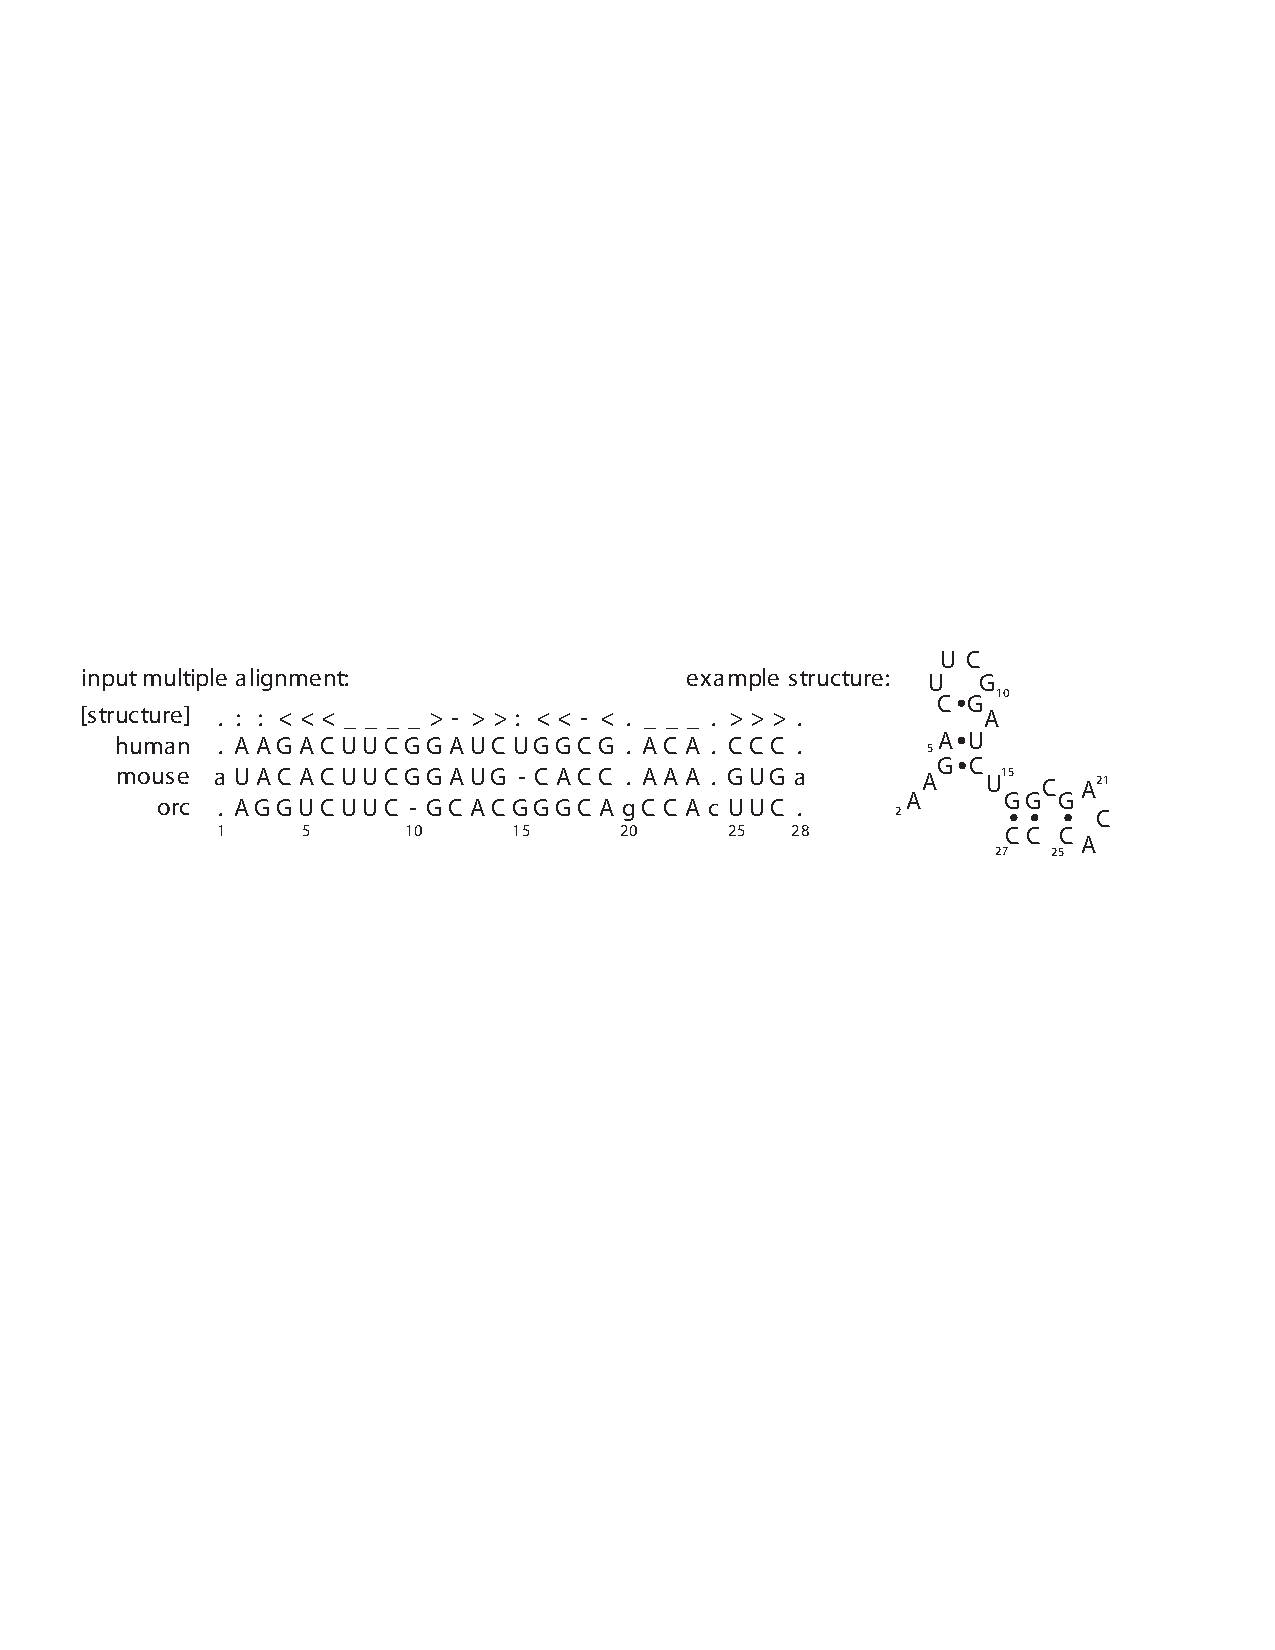
\includegraphics[scale=0.8]{Figures/input_alignment}
\end{center}
\caption{\small\textbf{An example RNA sequence family.} Left: a toy multiple
alignment of three sequences, with 28 total columns, 24 of which will
be modeled as consensus positions. The [structure] line annotates the
consensus secondary structure in WUSS notation.
Right: the secondary structure of the ``human'' sequence.} 
\label{fig:input_alignment}
\end{figure}

The guide tree has eight types of nodes:

\vspace{0.5em}
\begin{center}
\begin{tabular}{lll}
Node      & Description        &  Main state type          \\ \hline
MATP  & (pair)                 & P \\
MATL  & (single strand, left)  & L \\
MATR  & (single strand, right) & R \\
BIF   & (bifurcation)          & B \\
ROOT  & (root)                 & S \\
BEGL  & (begin, left)          & S \\
BEGR  & (begin, right)         & S \\
END   & (end)                  & E \\
\end{tabular}
\end{center}
\vspace{0.5em}
 
These consensus node types correspond closely with the CM's final
state types. Each node will eventually contain one or more states. The
guide tree deals with the consensus structure. For individual
sequences, we will need to deal with insertions and deletions with
respect to this consensus. The guide tree is the skeleton on which we
will organize the CM. For example, a MATP node will contain a P-type
state to model a consensus base pair; but it will also contain several
other states to model infrequent insertions and deletions at or
adjacent to this pair.

The input alignment is first used to construct a consensus secondary
structure (Figure~\ref{fig:cm_nodetree}) that defines which aligned
columns will be ignored as non-consensus (and later modeled as
insertions relative to the consensus), and which consensus alignment
columns are base-paired to each other. For the purposes of this
description, I assume that both the structural annotation and the
labeling of insert versus consensus columns is given in the input
file, as shown in the alignment in Figure~\ref{fig:input_alignment},
where both are are indicated by the WUSS notation in the [structure]
line (where, e.g., insert columns are marked with \verb+.+). (In
practice, \prog{cmbuild} does need secondary structure annotation, but
it doesn't require insert/consensus annotation or full WUSS notation
in its input alignment files; this would require a lot of manual
annotation.  More on this later.)

\begin{figure}[t]
\begin{center}
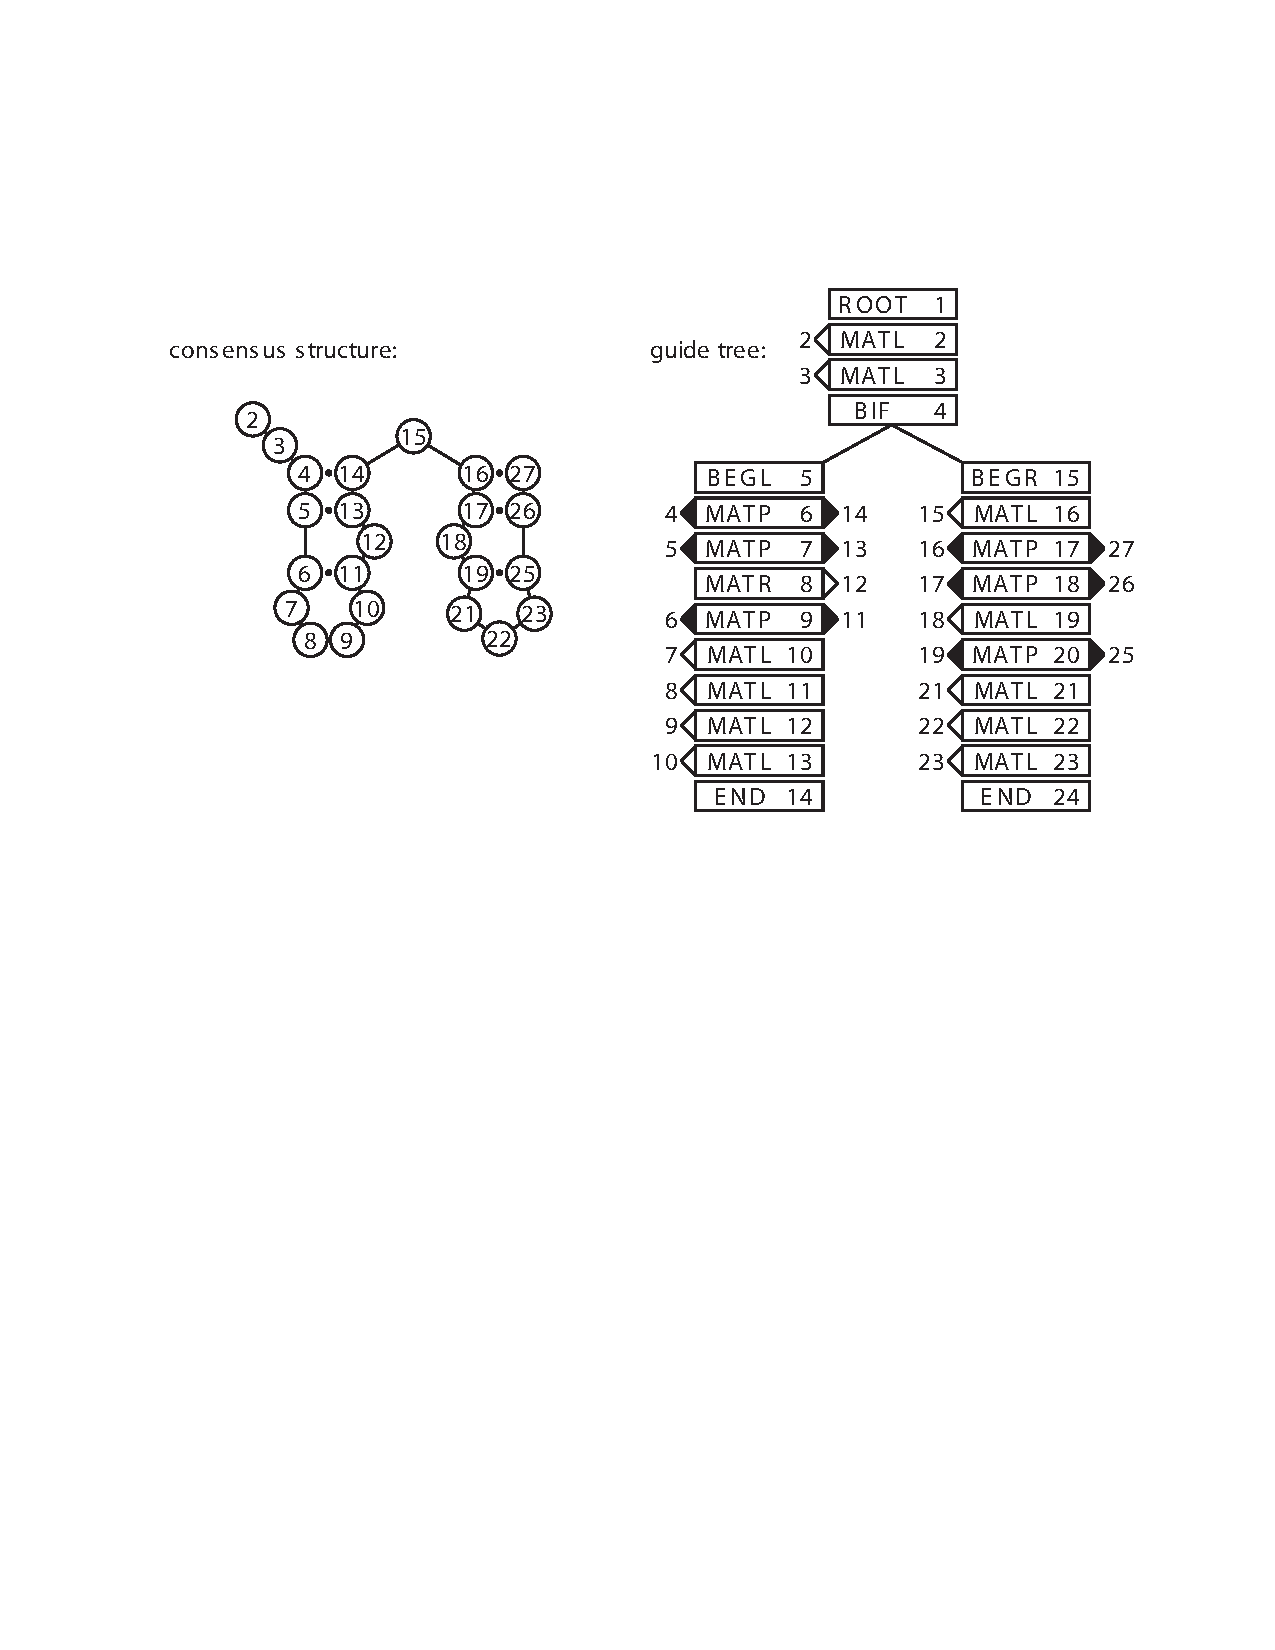
\includegraphics[width=5in]{Figures/cm_nodetree}
\end{center}
\caption{\small\textbf{The structural alignment is converted to a guide
tree.} Left: the consensus secondary structure is derived from the
annotated alignment in Figure~\ref{fig:input_alignment}. Numbers in
the circles indicate alignment column coordinates: e.g.  column 4 base
pairs with column 14, and so on. Right: the CM guide tree
corresponding to this consensus structure. The nodes of the tree are
numbered 1..24 in preorder traversal (see text). MATP, MATL, and MATR
nodes are associated with the columns they generate: e.g., node 6 is a
MATP (pair) node that is associated with the base-paired columns 4 and
14.}
\label{fig:cm_nodetree}
\end{figure}

Given the consensus structure, consensus base pairs are assigned to
MATP nodes and consensus unpaired columns are assigned to MATL or MATR
nodes. One ROOT node is used at the head of the tree.  Multifurcation
loops and/or multiple stems are dealt with by assigning one or more
BIF nodes that branch to subtrees starting with BEGL or BEGR head
nodes. (ROOT, BEGL, and BEGR start nodes are labeled differently
because they will be expanded to different groups of states; this has
to do with avoiding ambiguous parse trees for individual sequences, as
described below.) Alignment columns that are considered to be
insertions relative to the consensus structure are ignored at this
stage.

In general there will be more than one possible guide tree for any
given consensus structure. Almost all of this ambiguity is eliminated
by three conventions: (1) MATL nodes are always used instead of MATR
nodes where possible, for instance in hairpin loops; (2) in describing
interior loops, MATL nodes are used before MATR nodes; and (3) BIF
nodes are only invoked where necessary to explain branching secondary
structure stems (as opposed to unnecessarily bifurcating in single
stranded sequence). One source of ambiguity remains. In invoking a
bifurcation to explain alignment columns $i..j$ by two substructures
on columns $i..k$ and $k+1..j$, there will be more than one possible
choice of $k$ if $i..j$ is a multifurcation loop containing three or
more stems. The choice of $k$ impacts the performance of the divide
and conquer algorithm; for optimal time performance, we will want
bifurcations to split into roughly equal sized alignment problems, so
I choose the $k$ that makes $i..k$ and $k+1..j$ as close to the same
length as possible.

The result of this procedure is the guide tree. The nodes of the guide
tree are numbered in preorder traversal (e.g. a recursion of ``number
the current node, visit its left child, visit its right child'': thus
parent nodes always have lower indices than their children). The guide
tree corresponding to the input multiple alignment in
Figure~\ref{fig:input_alignment} is shown in
Figure~\ref{fig:cm_nodetree}.

\subsubsection{From guide tree to covariance model}

A CM must deal with insertions and deletions in individual sequences
relative to the consensus structure. For example, for a consensus base
pair, either partner may be deleted leaving a single unpaired residue,
or the pair may be entirely deleted; additionally, there may be
inserted nonconsensus residues between this pair and the next pair in
the stem. Accordingly, each node in the master tree is expanded into
one or more \emph{states} in the CM as follows:

\vspace{0.5em}
\begin{center}
\begin{tabular}{llccc}
       &                     & total \#& \# of split& \# of insert\\
Node   &  States             & states  & states     & states \\ \hline
MATP   & [MP ML MR D] IL IR  &   6     &   4        &  2   \\
MATL   & [ML D] IL           &   3     &   2    &  1   \\
MATR   & [MR D] IR           &   3     &   2    &  1   \\
BIF    & [B]                 &   1     &   1    &  0   \\
ROOT   & [S] IL IR           &   3     &   1    &  2   \\
BEGL   & [S]                 &   1     &   1    &  0   \\
BEGR   & [S] IL              &   2     &   1    &  1   \\
END    & [E]                 &   1     &   1    &  0   \\ \hline
\end{tabular}
\end{center}
\vspace{0.5em}

Here we distinguish between consensus (``M'', for ``match'') states
and insert (``I'') states. ML and IL, for example, are both L type
states with L type productions, but they will have slightly different
properties, as described below.

The states are grouped into a \emph{split set} of 1-4 states (shown in
brackets above) and an \emph{insert set} of 0-2 insert states. The
split set includes the main consensus state, which by convention is
first. One and only one of the states in the split set must be visited
in every parse tree (and this fact will be exploited by the divide and
conquer algorithm). The insert state(s) are not obligately visited,
and they have self-transitions, so they will be visited zero or more
times in any given parse tree.

State transitions are then assigned as follows. For bifurcation nodes,
the B state makes obligate transitions to the S states of the child
BEGL and BEGR nodes. For other nodes, each state in a split set has a
possible transition to every insert state in the \emph{same} node, and
to every state in the split set of the \emph{next} node. An IL state
makes a transition to itself, to the IR state in the same node (if
present), and to every state in the split set of the next node. An IR
state makes a transition to itself and to every state in the split set
of the next node.

This arrangement of transitions guarantees that (given the guide tree)
there is unambiguously one and only one parse tree for any given
individual structure. This is important. The algorithm will find a
maximum likelihood parse tree for a given sequence, and we wish to
interpret this result as a maximum likelihood structure, so there must
be a one to one relationship between parse trees and secondary
structures \cite{Giegerich00}.

The final CM is an array of $M$ states, connected as a directed graph
by transitions $t_v(y)$ (or probability 1 transitions $v \rightarrow
(y,z)$ for bifurcations) with the states numbered such that $(y,z)
\geq v$. There are no cycles in the directed graph other than cycles
of length one (e.g. the self-transitions of the insert states). We can
think of the CM as an array of states in which all transition
dependencies run in one direction; we can do an iterative dynamic
programming calculation through the model states starting with the
last numbered end state $M$ and ending in the root state $1$.  An
example CM, corresponding to the input alignment of
Figure~\ref{fig:input_alignment}, is shown in
Figure~\ref{fig:cm_graph}.

As a convenient side effect of the construction procedure, it is
guaranteed that the transitions from any state are to a
\emph{contiguous} set of child states, so the transitions for state
$v$ may be kept as an offset and a count. For example, in
Figure~\ref{fig:cm_graph}, state 12 (an MP) connects to states 16, 17,
18, 19, 20, and 21. We can store this as an offset of 4 to the first
connected state, and a total count of 6 connected states.  We know
that the offset is the distance to the next non-split state in the
current node; we also know that the count is equal to the number of
insert states in the current node, plus the number of split set states
in the next node. These properties make establishing the connectivity
of the CM trivial. Similarly, all the parents of any given state are
also contiguously numbered, and can be determined analogously. We are
also guaranteed that the states in a split set are numbered
contiguously.  This contiguity is exploited by the divide and conquer
implementation.

\begin{figure}[tp]
\begin{center}
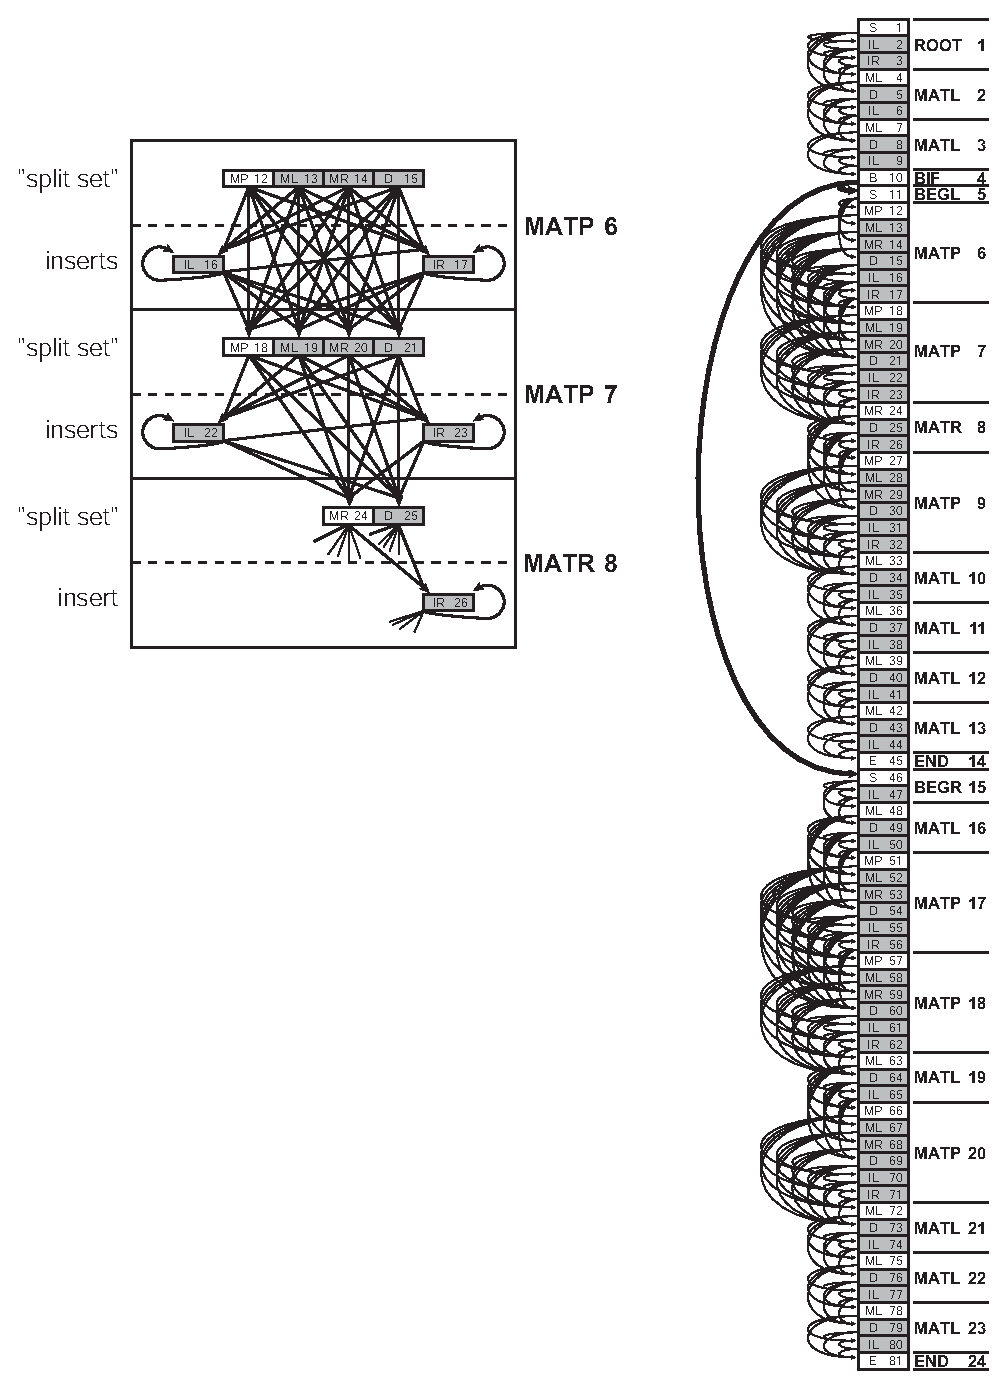
\includegraphics[width=5in]{Figures/cm_graph}
\end{center}
\caption{\small\textbf{A complete covariance model.} Right: the CM
corresponding to the alignment in Figure~\ref{fig:input_alignment}.
The model has 81 states (boxes, stacked in a vertical array). Each
state is associated with one of the 24 nodes of the guide tree (text
to the right of the state array). States corresponding to the
consensus are in white. States responsible for insertions and
deletions are gray. The transitions from bifurcation state B10 to
start states S11 and S46 are in bold because they are special: they
are an obligate (probability 1) bifurcation. All other transitions
(thin arrows) are associated with transition probabilities.  Emission
probability distributions are not represented in the figure. Left: the
states are also arranged according to the guide tree. A blow up of
part of the model corresponding to nodes 6, 7, and 8 shows
more clearly the logic of the connectivity of transition probabilities
(see main text), and also shows why any parse tree must transit through
one and only one state in each ``split set''.}
\label{fig:cm_graph}
\end{figure}

\subsubsection{Parameterization}

Using the guide tree and the final CM, each individual sequence in the
input multiple alignment can be converted unambiguously to a CM parse
tree, as shown in Figure~\ref{fig:parsetrees}. Weighted counts for
observed state transitions and singlet/pair emissions are then
collected from these parse trees. These counts are converted to
transition and emission probabilities, as maximum \emph{a posteriori}
estimates using mixture Dirichlet priors.

\begin{figure}[t]
\begin{center}
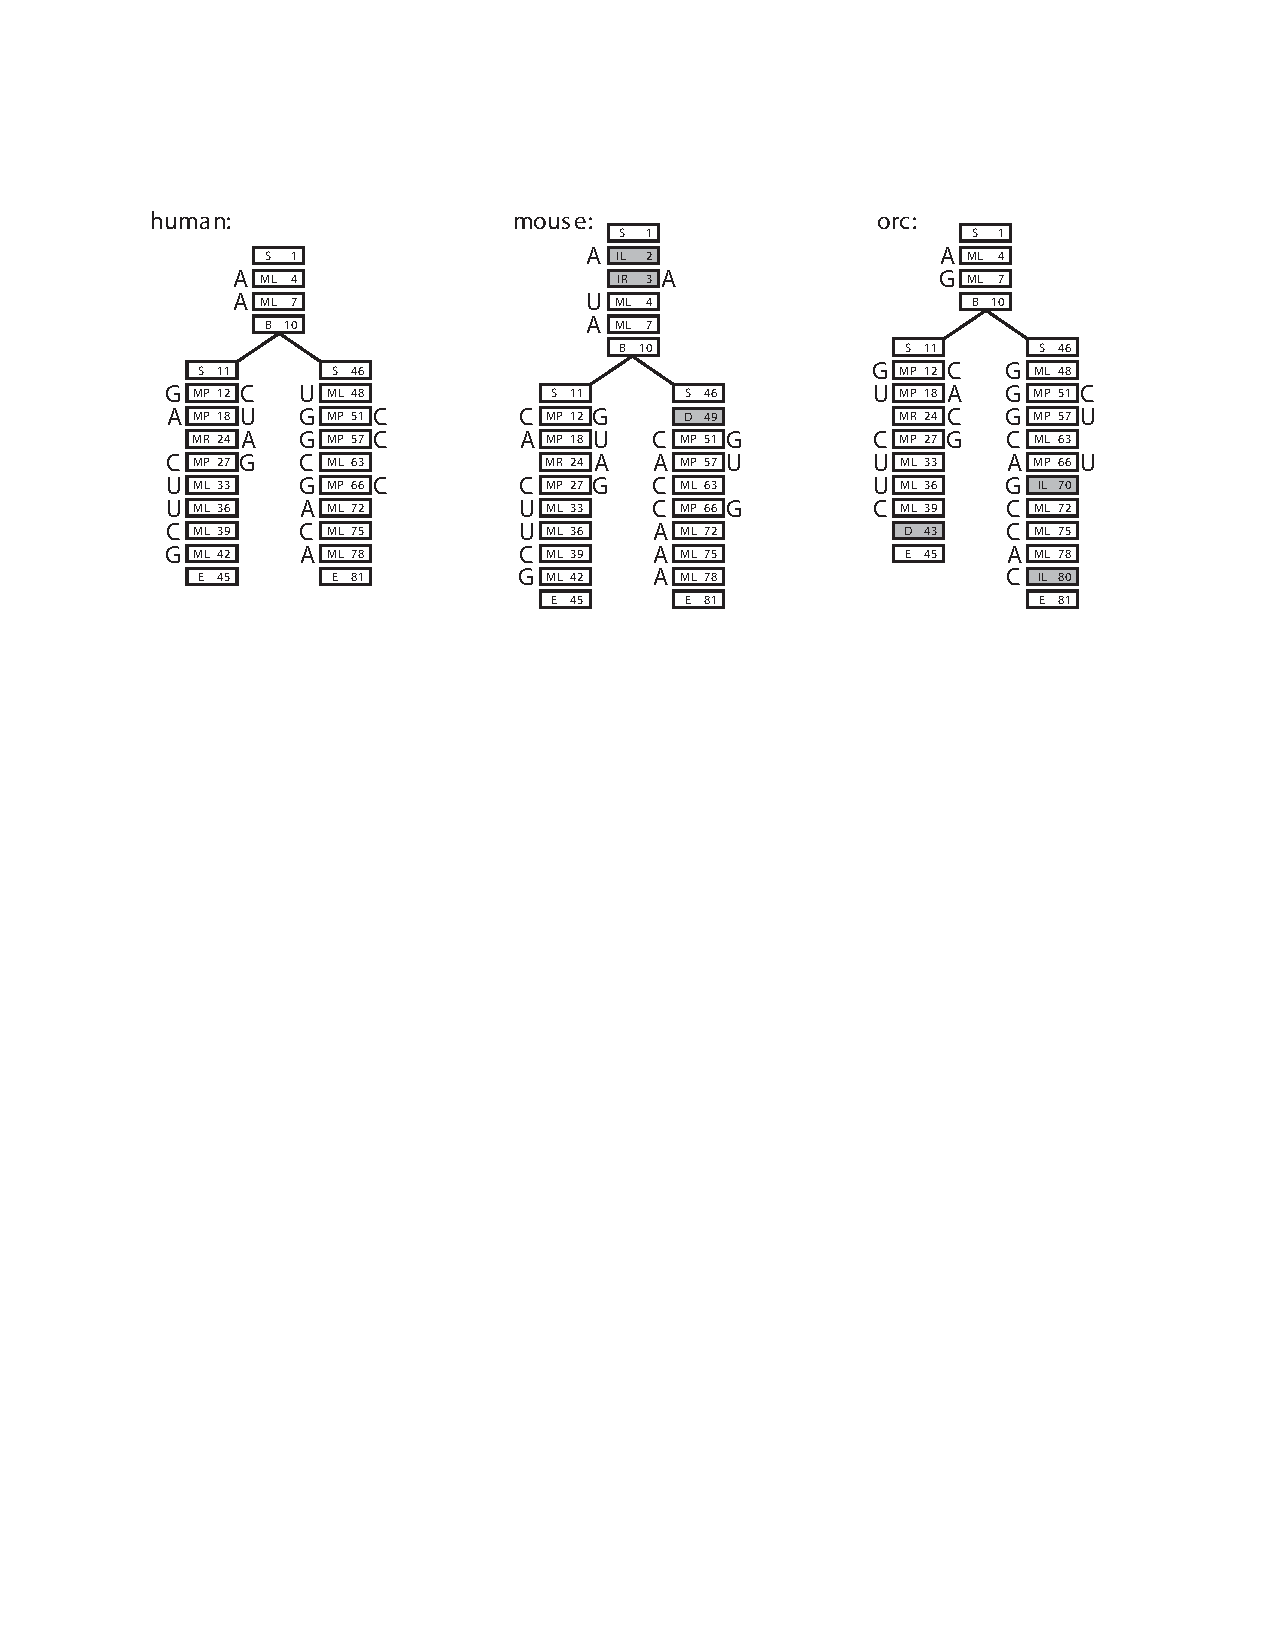
\includegraphics[width=5in]{Figures/parsetrees}
\end{center}
\caption{\small\textbf{Example parse trees.} Parse trees are shown for the
three sequences/structures from Figure~\ref{fig:input_alignment},
given the CM in Figure~\ref{fig:cm_graph}. For each sequence, each
residue must be associated with a state in the parse tree. (The
sequences can be read off its parse tree by starting at the upper left
and reading counterclockwise around the edge of parse tree.) Each
parse tree corresponds directly to a secondary structure -- base pairs
are pairs of residues aligned to MP states. A collection of parse
trees also corresponds to a multiple alignment, by aligning residues
that are associated with the same state -- for example, all three
trees have a residue aligned to state ML4, so these three residues
would be aligned together. Insertions and deletions relative to the
consensus use nonconsensus states, shown in gray.}
\label{fig:parsetrees}
\end{figure}

\subsubsection{Comparison to profile HMMs}

The relationship between an SCFG and a covariance model is analogous
to the relationship of hidden Markov models (HMMs) and profile HMMs
for modeling multiple sequence alignments
\cite{Krogh94,Durbin98,Eddy98}. A comparison may be instructive to
readers familiar with profile HMMs.  A profile HMM is a repetitive HMM
architecture that associates each consensus column of a multiple
alignment with a single type of model node -- a MATL node, in the
above notation. Each node contains a ``match'', ``delete'', and
``insert'' HMM state -- ML, IL, and D states, in the above notation.
The profile HMM also has special begin and end states. Profile HMMs
could therefore be thought of as a special case of CMs. An
unstructured RNA multiple alignment would be modeled by a guide tree
of all MATL nodes, and converted to an unbifurcated CM that would
essentially be identical to a profile HMM. (The only difference is
trivial; the CM root node includes a IR state, whereas the start node
of a profile HMM does not.) All the other node types (especially MATP,
MATR, and BIF) and state types (e.g. MP, MR, IR, and B) are SCFG
augmentations necessary to extend profile HMMs to deal with RNA
secondary structure.


\subsection{The \prog{cmbuild} program, step by step}
%\addtocontents{faq}{\textbf{Questions about using cmbuild:}}

The \prog{cmbuild} command line syntax is:

\user{cmbuild <options> [cmfile] [alifile]}

where \prog{[alifile]} is the name of the input alignment file, and
\prog{[cmfile]} is the name of the output CM file. What follows
describes the steps that \prog{cmbuild} goes through, and the most
important options that can be chosen to affect its behavior.

\subsubsection{Alignment input file}

The input alignment file must be in Stockholm format, and it must have
a consensus secondary structure annotation line (\verb+#=GC SS_cons+).

The program is actually capable of reading many common multiple
alignment formats (ClustalW, PHYLIP, GCG MSF, and others) but no other
format currently supports consensus RNA secondary structure
annotation. This may change in the future, either when other formats
allow structure annotation, or when \prog{cmbuild} is capable of
inferring consensus structure from the alignment by automated
comparative analysis, as the earlier \software{COVE} suite was capable
of \cite{Eddy94}. 

If the file does not exist, is not readable, or is not in a recognized
format, the program exits with a ``Alignment file doesn't exist or is
not readable'' error. If the file does not have consensus secondary
structure annotation, the program exits with a ``no consensus
structure annotation'' error. This includes all non-Stockholm
alignment files.

% EPN, Wed Apr  2 12:47:54 2008, the cat my.sto | cmbuild command
% in this faq no longer works.
\begin{comment}
\begin{srefaq}{Why does \prog{cmbuild} have a \prog{--informat} option, if it only
accepts Stockholm?} If you don't specify \prog{--informat}, the
software has to autodetect the file format. Autodetection of file
formats doesn't work in certain advanced/nonstandard cases, for
instance if you're reading the alignment from standard input instead
of from a file. The \prog{--informat} allows you to override
autodetection; e.g. \prog{cat my.sto | cmbuild --informat Stockholm
my.cm -} is an example of reading the alignment from piped standard
input.
\end{srefaq}
\end{comment}

\subsubsection{Parsing secondary structure annotation}

The structure annotation line only needs to indicate which columns are
base paired to which. It does not have to be in full WUSS notation.
Even if it is, the details of the notation are largely ignored.
Nested pairs of \verb+<>+, \verb+()+, \verb+[]+, or \verb+{}+ symbols
are interpreted as base paired columns. All other columns marked with
the symbols \verb+:,_-.~+ are interpreted as single stranded columns.

A simple minimal annotation is therefore to use \verb+<>+ symbols to
mark base pairs and \verb+.+ for single stranded columns.

If a secondary structure annotation line is in WUSS notation and it
contains valid pseudoknot annotation (e.g.\ additional non-nested
stems marked with AAA,aaa or BBB,bbb, etc.), this annotation is
ignored because \software{infernal} cannot handle
pseudoknots. Internally, these columns are treated as if they were
marked with \verb+.+ symbols.

\begin{srefaq}{How should I choose to annotate pseudoknots?} 
\software{infernal} can only deal with nested base pairs. If there is
a pseudoknot, you have to make a choice of which stem to annotate as
normal nested structure (thus including it in the model) and which
stem to call additional ``pseudoknotted'' structure (thus ignoring it
in the model). For example, for a simple two-stem pseudoknot, should
you annotate it as \verb+AAAA.<<<<aaaa....>>>>+, or
\verb+<<<<.AAAA>>>>....aaaa+?  From an RNA structure viewpoint, which
stem I label as the pseudoknotted one is an arbitrary choice; but
since one of the stems in the pseudoknot will have to be modeled as a
single stranded region by \software{infernal}, the choice makes a
slight difference in the performance of your model. You want your
model to capture as much information content as possible.  Thus, since
the information content of the model is a sum of the sequence
conservation plus the additional information contributed by pairwise
correlations in base-paired positions, you should tend to annotate the
shorter stem as the ``pseudoknot'' (modeling as many base pairs as
possible), and you should also annotate the stem with the more
conserved primary sequence as the ``pseudoknot'' (if one stem is more
conserved at the sequence level, you won't lose as much by modeling
that one as primary sequence consensus only).
\end{srefaq}

If (aside from any ignored pseudoknot annotation) the structure
annotation line contains characters other than \verb+<>()[]{}:_-,.~+
then those characters are ignored (treated as \verb+.+) and a warning
is printed.

If, after this ``data cleaning'', the structure annotation is
inconsistent with a secondary structure (for example, if the number of
\verb+<+ and \verb+>+ characters isn't the same), then the program
exits with a ``failed to parse consensus structure annotation'' error.

\subsubsection{Sequence weighting}

By default, the input sequences are weighted in two ways to compensate
for biased sampling (phylogenetic correlations).  Relative sequence
weights are calculated by the Gerstein/Chothia/Sonnhammer method
\cite{Gerstein94}.  (The \prog{--wgsc} option forces GSC weights, but
is redundant since that's the default.)  To turn relative weighting
off (e.g. set all weights to 1.0), use the \prog{--wnone} option.

Some alignment file formats allow relative sequence weights to be
given in the file. This includes Stockholm format, which has
\verb+#=GS WT+ weight annotations. Normally \prog{cmbuild} ignores any
such input weights.  The \prog{--wgiven} option tells \prog{cmbuild}
to use them.  This lets you set the weights with any external
procedure you like; for example, the \prog{weight} utility program in
\software{squid} implements some common weighting algorithms,
including the fast $O(N)$ Henikoff position-based weights
\cite{Henikoff94b}.

Absolute weights (the ``effective sequence number'') is calculate by
``entropy weighting'' \cite{Karplus98}. This sets the balance between
the prior and the data, and affects the information content of the
model. Entropy weighting reduces the effective sequence number (the
total sum of the weights) and increases the entropy (degrading the
information content) of the model until a threshold is reached. The
default entropy is 1.41 bits per position (roughly 0.59 bits of
information, relative to uniform base composition). This threshold can
be changed with the \prog{--ere <x>} option. Entropy weighting may
be turned off entirely with the \prog{--enone} option.


\subsubsection{Architecture construction}

The CM architecture is now constructed from your input alignment and
your secondary structure annotation, as described in the previous
section. 

The program needs to determine which columns are consensus (match)
columns, and which are insert columns. (Remember that although WUSS
notation allows insertions to be annotated in the secondary structure
line, \prog{cmbuild} is only paying attention to annotated base
pairs.) By default, it does this by a simple rule based on the
frequency of gaps in a column. If the frequency of gaps is greater
than a threshold, the column is considered to be an insertion. 

The threshold defaults to 0.5. It can be changed to another number
\verb+<x>+ (from 0 to 1.0) by the \prog{--gapthresh <x>} option.  The
higher the number, the more columns are included in the model.  At
\prog{--gapthresh 1.0}, all the columns are considered to be part of
the consensus. At \prog{--gapthresh 0.0}, only columns with no gaps are.

You can also manually specify which columns are consensus versus
insert by including reference coordinate annotation (e.g. a
\verb+#=GC RF+ line, in Stockholm format) and using the \prog{--rf}
option. Any columns marked by non-gap symbols become consensus
columns. (The simplest thing to do is mark consensus columns with x's,
and insert columns with \verb+.+'s. Remember that spaces aren't
allowed in alignments in Stockholm format.) If you set the \prog{--rf}
option but your file doesn't have reference coordinate annotation, the
program exits with an error.

\subsubsection{Parameterization}

Weighted observed emission and transition counts are then collected
from the alignment data. These count vectors $c$ are then converted to
estimated probabilities $p$ using mixture Dirichlet priors. The
default mixture priors are described in \cite{NawrockiEddy07}. You can
provide your own prior as a file, using the \prog{--prior <f>}
option.

\subsubsection{Naming the model}

Each CM gets a name. Stockholm format allows the alignment to have a
name, provided in the \verb+#=GF ID+ tag. If this name is provided,
it is used as the CM name.

Stockholm format allows more than one alignment per file, and
\prog{cmbuild} supports this: CM files can contain more than one
model, and if you say e.g.\ \prog{cmbuild Rfam.cm Rfam.sto} where
\verb+Rfam.sto+ contains a whole database of alignments,
\prog{cmbuild} will create a database of CMs in the \prog{Rfam.cm} file,
one per alignment. 

If a name or names are not provided in the Stockholm \verb+#=GF ID+
annotation, the name given to each CM is the input filename plus a ``-''
character and an integer indicating the position of that alignment
within the alignment file. For example, if you build a model from a
single alignment in alignment file \prog{RNaseP.sto}, the model will
be named RNaseP-1. 

If the \prog{--cmaxid, --ctarget} or \prog{--call} options are used to
split each input alignment into several alignments (see the
Tutorial for an example), then an additional extension of ``.''
plus an integer indicating the order in which the model was
constructed from the alignment is added to the name. For example, if
you run \prog{cmbuild --ctarget 3} with the alignment file
\prog{RNaseP.sto}, \prog{cmbuild} will cluster the alignment by
sequence identity into 3 clusters and build 3 CMs, one from each
cluster. These CMs will be named: RNaseP-1.1, RNaseP-1.2 and RNaseP-1.3.

If the alignment file only has 1 alignment in it, you can override the
automatic naming conventions and provide your own name with the \prog{-n <s>}
option, where \prog{<s>} is any string. 

\subsubsection{Saving the model}

The model is now saved to a file, according to the filename specified
on the command line. By default, a new file is created, and the model
is saved in a portable ASCII text format.

If the cmfile already exists, the program exits with an error. The
\prog{-F} option causes the new model to overwrite an existing
cmfile. The \prog{-A} option causes the new model to be appended to
an existing cmfile (creating a growing CM database, perhaps).



\newpage
\section{Tabular output formats}
\label{section:tabular}
\setcounter{footnote}{0}

\subsection{Target hits tables}

The \ccode{--tblout} output option in \prog{cmsearch} and
\prog{cmscan} produces \emph{target hits tables}. There are three
different formats of target hits table, which are both described
below. By default, both \prog{cmsearch} and \prog{cmscan} produce the
target hits table in \emph{format 1}. Format 1 is the only format that
was used by Infernal versions 1.1rc1 through 1.1.1. As of version
1.1.2, with \prog{cmscan}, the \ccode{--fmt 2} option can be used in
combination with \ccode{--tblout} to produce a target hits table in
the alternative \emph{format 2}.  As of version 1.1.5, with
\prog{cmscan} or \prog{cmsearch}, the \ccode{--fmt 3} option can be
used to add two additional fields (sequence length and model length)
to the standard format 1 files.  All three format target hits table
consist of one line for each different query/target comparison that
met the reporting thresholds, ranked by decreasing statistical
significance (increasing E-value).

\subsubsection{Target hits table format 1}

In the format 1 table, each line
consists of \textbf{18 space-delimited fields} followed by a free text
target sequence description, as follows:\footnote{The \ccode{tblout}
  format is deliberately space-delimited (rather than tab-delimited)
  and justified into aligned columns, so these files are suitable both
  for automated parsing and for human examination. Tab-delimited data
  files are difficult for humans to examine and spot check. For this
  reason, we think tab-delimited files are a minor evil in the
  world. Although we occasionally receive shrieks of outrage about
  this, we stubbornly feel that space-delimited files are just as
  trivial to parse as tab-delimited files.}

\begin{description}
\item[\emprog{(1) target name:}]
  The name of the target sequence or profile. 

\item[\emprog{(2) accession:}]
  The accession of the target sequence or profile, or '-' if none.

\item[\emprog{(3) query name:}] 
  The name of the query sequence or profile.

\item[\emprog{(4) accession:}]
  The accession of the query sequence or profile, or '-' if none.

\item[\emprog{(5) mdl (model):}] Which type of model was used to
  compute the final score. Either 'cm' or 'hmm'. A CM is
  used to compute the final hit scores unless the model has zero
  basepairs or the \ccode{--hmmonly} option is used, in which case a
  HMM will be used. 

\item[\emprog{(6) mdl from (model coord):}]
  The start of the alignment of this hit with respect to the
  profile (CM or HMM), numbered 1..N for a profile of N consensus positions.

\item[\emprog{(7) mdl to (model coord):}]
  The end of the alignment of this hit with respect to the
  profile (CM or HMM), numbered 1..N for a profile of N consensus positions.

\item[\emprog{(8) seq from (ali coord):}]
  The start of the alignment of this hit with respect to the
  sequence, numbered 1..L for a sequence of L residues.
 
\item[\emprog{(9) seq to (ali coord):}]
  The end of the alignment of this hit with respect to the
  sequence, numbered 1..L for a sequence of L residues.

\item[\emprog{(10) strand:}]
  The strand on which the hit occurs on the sequence. '+' if the hit is on
  the top (Watson) strand, '-' if the hit is on the bottom (Crick) strand.
  If on the top strand, the ``seq from'' value will be less than or
  equal to the ``seq to'' value, else it will be greater than or equal
  to it. 

\item[\emprog{(11) trunc:}] 
  Indicates if this is predicted to be a truncated CM hit or not. This will be
  ``no'' if it is a CM hit that is not predicted to be truncated by the end of the
  sequence, ``5'\,'' or ``3'\,'' if the hit is predicted to have one or more
  5' or 3' residues missing  due to a artificial truncation of the
  sequence, or ``5'\&3''' if the hit is predicted to have one or more
  5' residues missing and one or more 3' residues missing.
  If the hit is an HMM hit, this will always be '-'. 

\item[\emprog{(12) pass:}] 
  Indicates what ``pass'' of the pipeline the hit was detected
  on. This is probably only useful for testing and
  debugging. Non-truncated hits are found on the first pass, truncated
  hits are found on successive passes.

\item[\emprog{(13) gc:}] 
  Fraction of G and C nucleotides in the hit. 

\item[\emprog{(14) bias:}] The biased-composition correction: the bit
  score difference contributed by the null3 model for CM hits, or the
  null2 model for HMM hits. High bias scores may be a red flag for a
  false positive. It is difficult to correct for all possible ways in
  which a nonrandom but nonhomologous biological sequences can appear
  to be similar, such as short-period tandem repeats, so there are
  cases where the bias correction is not strong enough (creating false
  positives).

\item[\emprog{(15) score:}]
  The score (in bits) for this target/query comparison. It includes
  the biased-composition correction (the ``null3'' model for CM hits,
  or the ``null2'' model for HMM hits). 

\item[\emprog{(16) E-value:}] The expectation value (statistical
  significance) of the target.  This is a \emph{per query} E-value;
  i.e.\ calculated as the expected number of false positives achieving
  this comparison's score for a \emph{single} query against the search
  space $Z$. For \prog{cmsearch} $Z$ is defined as the total number of
  nucleotides in the target dataset multiplied by 2 because both strands
  are searched. For \prog{cmscan} $Z$ is the total number of
  nucleotides in the query sequence multiplied by 2 because both
  strands are searched and multiplied by the number of models in the target
  database. If you search with multiple queries and if you want to
  control the \emph{overall} false positive rate of that search rather
  than the false positive rate per query, you will want to multiply
  this per-query E-value by how many queries you're doing.

\item[\emprog{(17) inc:}] 
  Indicates whether or not this hit achieves the inclusion threshold:
  '!' if it does, '?' if it does not (and rather only achieves the
  reporting threshold). By default, the inclusion threshold is an
  E-value of 0.01 and the reporting threshold is an E-value of 10.0,
  but these can be changed with command line options as described in
  the manual pages.

\item[\emprog{(18) description of target:}] 
  The remainder of the line is the target's description line, as free text.
\end{description}

\subsubsection{Target hits table format 2}
\label{tabular-format2}

With the \prog{cmscan} program, the \ccode{--fmt 2} in combination with
\ccode{--tblout} option can be used to change the format of the
tabular output file for format 2 that includes additional information
on overlapping hits. Format 2 output is not possible from
\prog{cmsearch} because it is unable to calculate overlap information.
Format 2 includes all 18 of the fields from format 1 in the same order, plus 11
additional fields that are interspersed between some of the 18 from
format 1, as follows:

\begin{description}

\item[\emprog{(Before field 1 of format 1) idx:}] 
  The index of the hit in the list. The first hit has index '1', the
  second has index '2', the Nth hit has index 'N'.

\item[\emprog{(Before field 5 of format 1) clan name:}] 
  The name of the clan the model for this hit belongs to, or \ccode{-} if
  the model does not belong to a clan. A clan is a group of related
  models. For example, Rfam groups three LSU rRNA models
  (LSU\_rRNA\_archaea, LSU\_rRNA\_bacteria, and LSU\_rRNA\_eukarya)
  into the same clan. The value in this field will always be \ccode{-}
  unless the \ccode{--clanin <f>} option was used with
  \ccode{cmscan} to specify clan/model relationships in the input file
  \ccode{<f>}. See section~\ref{section:formats} for a description of
  the format of the input file used with \ccode{--clanin}.

\end{description}

The following nine fields all occur in format 2 between fields 17
('inc:') and 18 ('description of target') from format 1. 

\begin{description}

\item[\emprog{olp:}] A single character indicating the overlap status
  of this hit. Here, two hits are deemed to \emph{overlap} if they
  share at least one nucleotide on the same strand of the same
  sequence. There are four possible values in this field: \ccode{*},
  \ccode{\^}, \ccode{\$} and \ccode{=}.  \ccode{*} indicates this hit
  does not overlap with any other reported hits. \ccode{\^} indicates
  that this hit does overlap with at least one other hit, but none of
  the hits that overlap with it have a lower E-value (occur above it in
  the hit list). \ccode{\$} indicates that this hit does overlap with
  at least one other hit that does have a lower E-value (occurs above
  it in the hit list) but none of those higher scoring hits have
  \ccode{\^} in this column. \ccode{=} indicates that this hit does
  overlap with at least one other hit that has a lower E-value (occurs
  above it in the hit list) and does itself have a \ccode{\^} in this
  column. If the \ccode{--oclan} option was enabled, the definition of
  \emph{overlap} for the designations of the four characters
  \ccode{*}, \ccode{\^}, \ccode{\$} and \ccode{=} described above
  changes to: two hits are deemed to \emph{overlap} if they share at
  least one nucleotide on the same strand of the same sequence and
  they are to models that are in the same clan. That is, only overlaps
  between hits to models that are in the same clan are counted, all
  other overlaps are ignored and not annotated.  Infernal will never
  report two overlapping hits to the same model.

\item[\emprog{anyidx:}]
For hits that have \ccode{=} in the ``olp'' field, this is the
index of the lowest E-value hit that overlaps with this hit.
For hits with either \ccode{*} or \ccode{\^} in the ``olp'' field,
this field will always be \ccode{-}. For hits with \ccode{\$} in the 
``olp'' field, the hit referred to in this field will itself have
``='' in the ``olp'' field, or will be ``-1'' if that hit was skipped
(due to the ``--oskip'' option also having been used).

\item[\emprog{anyfrct1:}]
For hits that have \ccode{=} or \ccode{\$} in the ``olp'' field, this is the
fraction of the length of this hit that overlaps with the best scoring
overlapping hit (the hit index given in the ``anyidx'' field), to
4 significant digits. 
For hits with \ccode{-} in the ``anyidx''
field, this field will always be \ccode{-}.  

\item[\emprog{anyfrct2:}]
For hits that have \ccode{=} or \ccode{\$} in the ``olp'' field, this is the
fraction of the length of the best scoring overlapping hit (the hit
index given in the ``anyidx'' field) that overlaps with this hit,
to 4 significant digits. 
For hits with \ccode{-} in the ``anyidx''
field, this field will always be \ccode{-}.  

\item[\emprog{winidx:}] 
For hits that have \ccode{=} in the ``olp'' field, this is either
\ccode{"} or the index of the best scoring hit that overlaps with this
hit that is marked as \ccode{\^} in the ``olp'' field. If the value
is \ccode{"} it means that the best scoring hit that overlaps with
this hit that is marked as \ccode{\^} in the ``olp'' field is
already listed in the ``anyidx'' field, which is usually the case.
For hits with either \ccode{*}, \ccode{\^} or \ccode{\$} in the ``olp'' field,
this field will always be \ccode{-}.

\item[\emprog{winfrct1:}]
For hits that have neither \ccode{-} nor \ccode{"} in the
``winidx'' field, this is the fraction of the length of this hit
that overlaps with the best scoring overlapping hit marked with
\ccode{\^} in the ``olp'' field (the hit index given in the
``winidx'' field), to 4 significant digits.  For hits with either
\ccode{*}, \ccode{\^} or \ccode{\$} in the ``olp'' field, this field will
always be \ccode{-}.  For hits with \ccode{-} in the ``winidx''
field, this field will always be \ccode{-}.  
For hits with \ccode{"} in the ``winidx''
field, this field will always be \ccode{"}.  

\item[\emprog{winfrct2:}]
For hits that have neither \ccode{-} nor \ccode{"} in the
``"winidx'' field, this is the
fraction of the length of the best scoring overlapping hit marked with
\ccode{\^} in the ``olp'' field (the hit
index given in the ``winidx'' field) that overlaps with this hit,
to 4 significant digits. 
For hits with either 
\ccode{*}, \ccode{\^} or \ccode{\$} in the ``olp'' field, this field will
always be \ccode{-}.  For hits with \ccode{-} in the ``winidx''
field, this field will always be \ccode{-}.  
For hits with \ccode{"} in the ``winidx''
field, this field will always be \ccode{"}.  

\item[\emprog{mdl len:}]
The consensus length of the profile (CM or HMM) for this hit.

\item[\emprog{seq len:}]
The total length of the sequence for this hit.

\end{description}

\subsubsection{Target hits table format 3}
\label{tabular-format3}

With the \prog{cmsearch} and \prog{cmscan} programs, the \ccode{--fmt 3} 
in combination with \ccode{--tblout} option can be used to change
the format of the tabular output file to format 3 that includes all of
the fields in format 1 with two additional fields: the full length of
the sequence and model involved in each hit. The first 17 fields of
format 3 are identical to format 1, followed by the two additional
fields, and the final field is the ``description'' field from format
1. The two additional fields are:

\begin{description}

\item[\emprog{mdl len:}]
The consensus length of the profile (CM or HMM) for this hit.

\item[\emprog{seq len:}]
The total length of the sequence for this hit.

\end{description}

The tables are columnated neatly for human readability, but do not
write parsers that rely on this columnation; rely on space-delimited
fields. The pretty columnation assumes fixed maximum widths for each
field. If a field exceeds its allotted width, it will still be fully
represented and space-delimited, but the columnation will be disrupted
on the rest of the row.

Note the use of target and query columns. A program like
\prog{cmsearch} searches a query profile against a target sequence
database. In an \prog{cmsearch} tblout file, the sequence (target)
name is first, and the profile (query) name is second. A program like
\prog{cmscan}, on the other hand, searches a query sequence against a
target profile database. In a \prog{cmscan} tblout file, the profile
name is first, and the sequence name is second. You might say, hey,
wouldn't it be more consistent to put the profile name first and the
sequence name second (or vice versa), so \prog{cmsearch} and
\prog{cmscan} tblout files were identical? Well, they
still wouldn't be identical, because the target database size used for
E-value calculations is different (total number of target nucleotides
for \prog{cmsearch}, number of target profiles times target sequence
length for \prog{cmscan}), and it's good not to forget this.

If some of the descriptions of these fields don't make sense to you,
it may help to go through the tutorial in
section~\ref{section:tutorial} and read section~\ref{section:pipeline}
of the manual. 



% Changes in options between 1.0 and 1.1 are omitted from the 1.1.2 user guide.
%\newpage
%\section{Changes in command-line options from version 1.0}
\label{section:options}
\setcounter{footnote}{0}

The following tables list options from Infernal version 1.0 programs
that have either been removed, renamed or significantly changed in
version 1.1. Many options in cmsearch and cmcalibrate have changed or
been removed, mainly because the new search pipeline (see
section~\ref{section:pipeline}) is so different from the version 1.0
pipeline. For example the version 1.0 pipeline set HMM filter
thresholds for a search in a model-dependent manner, whereas those
thresholds are model-independent in version 1.1. Also, cmalign and
cmstat in version 1.1 are significantly simpler than they were in
version 1.0 and have many fewer options. The motivation for renaming
options whose behavior did not change was for consistency with
HMMER3, so that analogous options in Infernal and HMMER have the same
name. For more information on the version 1.1 options, see the manual
pages in this guide.

\subsection{cmalign options from Infernal version 1.0.x that have changed in version 1.1.} 

\begin{tabular}{|lll|}
\hline
%\multicolumn{3}{|l|}{\prog{cmalign} options in Infernal version 1.0 that have changed in version 1.1.} \\ \hline
                       & corresponding            &                                     \\
v1.0 option            & v1.1 option              & explanation                         \\ \hline
\otext{-1}             & \otext{--outformat pfam} & renamed only; no change in behavior \\
\otext{--banddump <n>} & none                     & no longer supported \\
\otext{--beta}         & none                     & QDB alignment is no longer supported \\
\otext{--checkfb}      & none                     & no longer supported \\
\otext{--checkpost}    & none                     & no longer supported \\
\otext{--devhelp}      & none                     & no longer necessary \\
\otext{--dlev}         & none                     & no longer supported \\
\otext{--dna}          & \otext{--dnaout}         & renamed only; no change in behavior \\
\otext{--fins}         & none                     & no longer supported \\
\otext{--gapthresh}    & none                     & no longer necessary \\
\otext{--hsafe}        & none                     & no longer supported \\
\otext{--inside}       & none                     & no longer supported \\
\otext{-l}             & none                     & true by default, local alignment is now the default behavior \\
none                   & \otext{-g}               & for global alignment, use \otext{-g} \\
\otext{--merge}        & none                     & no longer supported \\
\otext{--no-null3}     & none                     & no longer supported \\
\otext{--onepost}      & none                     & no longer supported \\
\otext{-p}             & none                     & true by default \\
none                   & \otext{--noprob}         & disable posterior probability annotation with \otext{--noprob} \\
\otext{-q}             & none                     & true by default, output scores with \otext{-o} or \otext{--sfile} \\
\otext{--qdb}          & none                     & QDB alignment is no longer supported \\
\otext{--pbegin <x>}   & none                     & no longer supported; settable for a CM in \otext{cmbuild} \\
\otext{--pebegin}      & none                     & no longer supported; settable for a CM in \otext{cmbuild} \\
\otext{--pend <x>}     & none                     & no longer supported; settable for a CM in \otext{cmbuild} \\
\otext{--pfend <x>}    & none                     & no longer supported; settable for a CM in \otext{cmbuild} \\
\otext{--resonly}      & none                     & no longer supported \\
\otext{--rf}           & none                     & no longer necessary \\
\otext{--rna}          & none                     & RNA output is true by default \\
\otext{-s}             & \otext{--seed}           & renamed only; no change in behavior \\
\otext{--sums}         & none                     & no longer supported \\
\otext{--viterbi}      & none                     & no longer supported \\
\otext{--withali <f>}  & \otext{--mapali <f>}     & \otext{<f>} must now be same alignment used to build CM \\
\otext{--withpknots}   & \otext{--withstr}        & renamed only; no change in behavior \\
\hline
\end{tabular}

\subsection{cmbuild options from Infernal version 1.0.x that have changed in version 1.1.} 

\begin{tabular}{|lll|}
\hline
%\multicolumn{3}{|l|}{\prog{cmalign} options in Infernal version 1.0 that have changed in version 1.1.} \\ \hline
                       & corresponding            &                                     \\
v1.0 option            & v1.1 option              & explanation                         \\ \hline
\otext{-a}             & \otext{--indi}           & renamed only; no change in behavior \\
\otext{-A}             & none                     & no longer supported \\
\otext{--eX}           & none                     & no longer supported \\
\otext{--gapthresh <x>}& \otext{--symfrac <y>}    & renamed; IMPORTANT: use \otext{<y>} equal to \otext{1.0-<x>} \\
                       &                          & where \otext{<x>} is from \otext{--gapthresh <x>} in v1.0 \\
\otext{--ignorant}     & \otext{--noss}           & renamed             \\
\otext{--pbswitch}     & none                     & no longer supported \\
\otext{-s}             & \otext{--seed}           & renamed only; no change in behavior \\
\otext{--rf}           & \otext{--hand}           & renamed only; no change in behavior \\
\otext{--regress}      & none                     & no longer supported \\
\otext{-v}             & \otext{--verbose}        & renamed             \\
\otext{--Wbeta <f>}    & \otext{--betaW}          & renamed only; no change in behavior \\
\hline
\end{tabular}


\subsection{cmcalibrate options from Infernal version 1.0.x that have changed in version 1.1.} 

\begin{tabular}{|lll|}
\hline
%\multicolumn{3}{|l|}{\prog{cmalign} options in Infernal version 1.0 that have changed in version 1.1.} \\ \hline
                             & corresponding            &                                     \\
v1.0 option                  & v1.1 option              & explanation                         \\ \hline
\otext{--devhelp}            & none                     & no longer necessary \\
\otext{--exp-beta <x>}       & \otext{--beta <x>}       & renamed only; no change in behavior \\
\otext{--exp-cmL-glc <x>}    & \otext{-L <x>}           & renamed \\
\otext{--exp-cmL-loc <x>}    & \otext{-L <x>}           & renamed \\
\otext{--exp-ffile <f>}      & \otext{--ffile <f>}      & renamed only; no change in behavior \\
\otext{--exp-fract}          & none                     & no longer relevant; HMMs are not calibrated \\
\otext{--exp-gc <f>}         & \otext{--gc}             & renamed only; no change in behavior \\
\otext{--exp-hfile <f>}      & \otext{--hfile <f>}      & renamed only; no change in behavior \\
\otext{--exp-hmmLn-glc <x>}  & none                     & no longer necessary; HMMs are not calibrated \\
\otext{--exp-hmmLn-loc <x>}  & none                     & no longer necessary; HMMs are not calibrated \\
\otext{--exp-hmmLx <x>}      & none                     & no longer necessary; HMMs are not calibrated \\
\otext{--exp-no-qdb}         & \otext{--noqdb}          & renamed only; no change in behavior \\
\otext{--exp-pfile <f>}      & none                     & no longer supported \\
\otext{--exp-qqfile <f>}     & \otext{--qqfile <f>}     & renamed only; no change in behavior \\
\otext{--exp-random}         & \otext{--random}         & renamed only; no change in behavior \\
\otext{--exp-sfile <f>}      & \otext{--sfile <f>}      & renamed only; no change in behavior \\
\otext{--exp-tailn-cglc}     & \otext{--gtailn}         & renamed \\
\otext{--exp-tailn-cloc}     & \otext{--ltailn}         & renamed \\
\otext{--exp-tailn-hglc <x>} & none                     & no longer necessary; HMMs are not calibrated \\
\otext{--exp-tailn-hloc <x>} & none                     & no longer necessary; HMMs are not calibrated \\
\otext{--exp-tailp}          & \otext{--tailp}          & renamed \\
\otext{--exp-tailxn}         & none                     & no longer supported \\
\otext{--exp-T <x>}          & none                     & no longer supported \\
\otext{--fil-aln2bands}      & none                     & no longer necessary; HMM filter thresholds no longer used \\
\otext{--fil-dfile}          & none                     & no longer necessary; HMM filter thresholds no longer used \\
\otext{--fil-gemit}          & none                     & no longer necessary; HMM filter thresholds no longer used \\
\otext{--fil-F <x>}          & none                     & no longer necessary; HMM filter thresholds no longer used \\
\otext{--fil-N <n>}          & none                     & no longer necessary; HMM filter thresholds no longer used \\
\otext{--fil-nonbanded}      & none                     & no longer necessary; HMM filter thresholds no longer used \\
\otext{--fil-Smax-hmm <x>}   & none                     & no longer necessary; HMM filter thresholds no longer used \\
\otext{--fil-Smin-hmm <x>}   & none                     & no longer necessary; HMM filter thresholds no longer used \\
\otext{--fil-Starg-hmm <x>}  & none                     & no longer necessary; HMM filter thresholds no longer used \\
\otext{--fil-tau <x>}        & none                     & no longer necessary; HMM filter thresholds no longer used \\
\otext{--fil-Xmin-hmm <x>}   & none                     & no longer necessary; HMM filter thresholds no longer used \\
\otext{--fil-Xtarg-hmm <x>}  & none                     & no longer necessary; HMM filter thresholds no longer used \\
\otext{--forecast <n>}       & \otext{--forecast}       & no longer takes \# of processors \otext{<n>}; use in combination\\
                             &                          & with \otext{--nforecast <n>} to reproduce v1.0 behavior \\
\otext{--mxsize}             & none                     & no longer supported \\
\otext{--no-null3}           & \otext{--nonull3}        & renamed only; no change in behavior \\
\otext{--pbegin <x>}         & none                     & no longer supported; settable for a CM in \otext{cmbuild} \\
\otext{--pebegin}            & none                     & no longer supported; settable for a CM in \otext{cmbuild} \\
\otext{--pend <x>}           & none                     & no longer supported; settable for a CM in \otext{cmbuild} \\
\otext{--pfend <x>}          & none                     & no longer supported; settable for a CM in \otext{cmbuild} \\
\otext{-s}                   & \otext{--seed}           & renamed only; no change in behavior \\
\otext{-v}                   & none                     & no longer supported \\
\hline
\end{tabular}


\subsection{cmemit options from Infernal version 1.0.x that have changed in version 1.1.} 

\begin{tabular}{|lll|}
\hline
%\multicolumn{3}{|l|}{\prog{cmalign} options in Infernal version 1.0 that have changed in version 1.1.} \\ \hline
                       & corresponding            &                                     \\
v1.0 option            & v1.1 option              & explanation                         \\ \hline
\otext{-n}             & \otext{-N}               & renamed only; no change in behavior \\
\otext{-s}             & \otext{--seed}           & renamed only; no change in behavior \\
\otext{--begin <n>}    & \otext{--a5p <n>}        & renamed only; no change in behavior \\
\otext{--end <n>}      & \otext{--a3p <n>}        & renamed only; no change in behavior \\
\otext{--shmm}         & none                     & no longer supported \\
\otext{--ahmm}         & none                     & no longer supported \\
\otext{--pbegin <x>}   & none                     & no longer supported; settable for a CM in \otext{cmbuild} \\
\otext{--pebegin}      & none                     & no longer supported; settable for a CM in \otext{cmbuild} \\
\otext{--pend <x>}     & none                     & no longer supported; settable for a CM in \otext{cmbuild} \\
\otext{--pfend <x>}    & none                     & no longer supported; settable for a CM in \otext{cmbuild} \\
\hline
\end{tabular}


\subsection{cmsearch options from Infernal version 1.0.x that have changed in version 1.1.} 

\begin{tabular}{|lll|}
\hline
%\multicolumn{3}{|l|}{\prog{cmalign} options in Infernal version 1.0 that have changed in version 1.1.} \\ \hline
                           & corresponding            &                                     \\
v1.0 option                & v1.1 option              & explanation                         \\ \hline
\otext{--aln2hbands}       & none                     & no longer supported \\
\otext{--aln-hbanded}      & none                     & true by default \\
\otext{--aln-optacc}       & none                     & true by default \\
\otext{--dna}              & none                     & no longer supported \\
\otext{--fil-no-hmm}       & \otext{--nohmm}          & renamed \\
\otext{--fil-no-qdb}       & \otext{--max}            & \otext{--max} turns off all filters \\
\otext{--fil-beta <x>}     & \otext{--fbeta <x>}      & renamed \\
\otext{--fil-A-hmm <x>}    & none                     & no longer supported \\
\otext{--fil-finE-hmm <x>} & none                     & no longer supported \\
\otext{--fil-finE-qdb <x>} & none                     & no longer supported \\
\otext{--fil-finT-hmm <x>} & none                     & no longer supported \\
\otext{--fil-finT-qdb <x>} & none                     & no longer supported \\
\otext{--fil-E-hmm <x>}    & none                     & no longer supported \\
\otext{--fil-E-qdb <x>}    & none                     & no longer supported \\
\otext{--fil-S-hmm <x>}    & none                     & no longer supported \\
\otext{--fil-Smax-hmm <x>} & none                     & no longer supported \\
\otext{--fil-Smin-hmm <x>} & none                     & no longer supported \\
\otext{--fil-T-hmm <x>}    & none                     & no longer supported \\
\otext{--fil-T-qdb <x>}    & none                     & no longer supported \\
\otext{--fil-Xmin-hmm <x>} & none                     & no longer supported \\
\otext{--forecast <n>}     & none                     & no longer supported \\
\otext{--forward}          & \otext{--hmmonly}        & renamed \\
\otext{--ga}               & \otext{--cut\_ga}        & renamed only; no change in behavior \\
\otext{--gcfile <f>}       & none                     & no longer supported \\
\otext{--hbanded}          & none                     & true by default \\
\otext{--hmm-W <n>}        & none                     & no longer supported \\
\otext{--hmm-cW <x>}       & \otext{--wcx <x>}        & renamed \\
\otext{--informat <s>}     & \otext{--tformat <s>}    & renamed only; no change in behavior \\
\otext{--inside}           & none                     & true by default \\
\otext{--lambda <x>}       & none                     & no longer supported \\
\otext{--nc}               & \otext{--cut\_nc}        & renamed only; no change in behavior \\
\otext{--noalign}          & \otext{--noali}          & renamed \\
\otext{--no-qdb}           & \otext{--nonbanded}      & renamed only; no change in behavior \\
\otext{--tabfile <f>}      & \otext{--tblout <f>}     & renamed, and format of \otext{<f>} changed \\
\otext{--tc}               & \otext{--cut\_tc}        & renamed only; no change in behavior \\
\otext{--no-null3}         & \otext{--nonull3}        & renamed only; no change in behavior \\
\otext{--null2}            & none                     & no longer supported \\
\otext{-p}                 & none                     & true by default \\
\otext{--pbegin <x>}       & none                     & no longer supported; settable for a CM in \otext{cmbuild} \\
\otext{--pebegin}          & none                     & no longer supported; settable for a CM in \otext{cmbuild} \\
\otext{--pend <x>}         & none                     & no longer supported; settable for a CM in \otext{cmbuild} \\
\otext{--pfend <x>}        & none                     & no longer supported; settable for a CM in \otext{cmbuild} \\
\otext{--rna}              & none                     & true by default \\
\otext{--rtrans}           & none                     & no longer supported \\
\otext{-v}                 & none                     & no longer supported \\
\otext{--viterbi}          & none                     & no longer supported \\
\otext{-x}                 & none                     & no longer supported \\
\hline
\end{tabular}


\subsection{cmstat options from Infernal version 1.0.x that have changed in version 1.1.} 

\begin{tabular}{|lll|}
\hline
%\multicolumn{3}{|l|}{\prog{cmalign} options in Infernal version 1.0 that have changed in version 1.1.} \\ \hline
                           & corresponding            &                                     \\
v1.0 option                & v1.1 option              & explanation                         \\ \hline
\otext{-g}                 & none                     & no longer relevant\\
\otext{-m}                 & none                     & true by default \\
\otext{--le}               & none                     & no longer supported \\
\otext{--ge}               & none                     & no longer supported \\
\otext{--beta <x>}         & none                     & no longer relevant \\
\otext{--qdbfile <x>}      & none                     & no longer supported \\
\otext{--lfi}              & none                     & no longer relevant \\
\otext{--gfi}              & none                     & no longer relevant \\
\otext{--lfc}              & none                     & no longer relevant \\
\otext{--gfc}              & none                     & no longer relevant \\
\otext{-E <x>}             & none                     & \otext{-E <x>} behaves differently now \\
\otext{-T <x>}             & none                     & \otext{-T <x>} behaves differently now \\
\otext{--nc}               & none                     & no longer relevant \\
\otext{--ga}               & none                     & no longer relevant \\
\otext{--tc}               & none                     & no longer relevant \\
\otext{--seqfile <f>}      & none                     & no longer supported \\
\otext{--toponly}          & none                     & no longer supported \\
\otext{--search}           & none                     & no longer supported \\
\otext{--cmL}              & none                     & no longer supported \\
\otext{--hmmL}             & none                     & no longer supported \\
\otext{--efile <f>}        & none                     & no longer relevant \\
\otext{--bfile <f>}        & none                     & no longer relevant \\
\otext{--sfile <f>}        & none                     & no longer relevant \\
\otext{--xfile <f>}        & none                     & no longer relevant \\
\otext{--afile <f>}        & none                     & no longer relevant \\
\otext{--bits}             & none                     & no longer relevant \\
\hline
\end{tabular}


\newpage
\section{Some other topics}
\label{section:more}
\setcounter{footnote}{0}

\subsection{How do I cite Infernal?}

If you'd like to cite a paper, please cite the Infernal 1.1 application
note in \emph{Bioinformatics}:

Infernal 1.1: 100-fold faster RNA homology searches.
EP Nawrocki and SR Eddy.
Bioinformatics, 29:2933-2935, 2013.

The most appropriate citation is to the web site,
\url{infernal.janelia.org}. You should also cite what version of the
software you used. We archive all old versions, so anyone should be
able to obtain the version you used, when exact reproducibility of an
analysis is an issue.

The version number is in the header of most output files. To see it
quickly, do something like \prog{cmscan -h} to get a help page, and
the header will say:

\begin{sreoutput}
# cmscan :: search sequence(s) against a CM database
# INFERNAL 1.1.1 (July 2014)
# Copyright (C) 2014 Howard Hughes Medical Institute.
# Freely distributed under the GNU General Public License (GPLv3).
# - - - - - - - - - - - - - - - - - - - - - - - - - - - - - - - - - - - -
\end{sreoutput}

So (from the second line there) this is from Infernal 1.1.1.

\subsection{How do I report a bug?}

Email us, at \url{infernal@janelia.hhmi.org}.

Before we can see what needs fixing, we almost always need to
reproduce a bug on one of our machines. This means we want to have a
small, reproducible test case that shows us the failure you're seeing.
So if you're reporting a bug, please send us:

\begin{itemize}
 \item A brief description of what went wrong.
 \item The command line(s) that reproduce the problem.
 \item Copies of any files we need to run those command lines.
 \item Information about what kind of hardware you're on, what
   operating system, and (if you compiled the software yourself rather
   than running precompiled binaries), what compiler and version you
   used, with what configuration arguments.
\end{itemize}

Depending on how glaring the bug is, we may not need all this
information, but any work you can put into giving us a clean
reproducible test case doesn't hurt and often helps.

The information about hardware, operating system, and compiler is
important. Bugs are frequently specific to particular configurations
of hardware/OS/compiler.  We have a wide variety of systems available
for trying to reproduce bugs, and we'll try to match your system as
closely as we can.

If you first see a problem on some huge compute (like running a
zillion query sequence over a huge profile database), it will really,
really help us if you spend a bit of time yourself trying to isolate
whether the problem really only manifests itself on that huge compute,
or if you can isolate a smaller test case for us. The ideal bug report
(for us) gives us everything we need to reproduce your problem in one
email with at most some small attachments. 

Remember, we're not a company with dedicated support staff -- we're a
small lab of busy researchers like you. Somebody here is going to drop
what they're doing to try to help you out. Try to save us some time,
and we're more likely to stay in our usual good mood.

If we're in our usual good mood, we'll reply quickly.  We'll probably
tell you we fixed the bug in our development code, and that the fix
will appear in the next Infernal release. This of course doesn't help you
much, since nobody knows when the next Infernal release is going to be.
So if possible, we'll usually try to describe a workaround for the
bug.

If the code fix is small, we might also tell you how to patch and
recompile the code yourself. You may or may not want to do this.

There are currently not enough open bugs to justify having a formal
on-line bug tracking system. We have a bugtracking system, but it's
internal.

\subsection{Input files}

\subsubsection{Reading from a stdin pipe using - (dash) as a filename argument}

Generally, Infernal programs read their sequence and/or profile input
from files. Unix power users often find it convenient to string an
incantation of commands together with pipes (indeed, such wizardly
incantations are a point of pride). For example, you might extract a
subset of query sequences from a larger file using a one-liner
combination of scripting commands (perl, awk, whatever). To facilitate
the use of Infernal programs in such incantations, you can almost
always use an argument of '-' (dash) in place of a filename, and the
program will take its input from a standard input pipe instead of
opening a file.\footnote{An important exception is the use of '-' in
place of the target sequence file in \prog{cmsearch}. This is not
allowed because \prog{cmsearch} first quickly reads the target
sequence file to determine its size (it needs to know this to know how
to set filter thresholds), then rewinds it and starts to process
it. There's a couple of additional cases where stdin piping won't work
described later in this section.}

For example, the following three commands are entirely equivalent, and
give essentially identical output:

\user{cmalign tRNA5.cm mrum-tRNAs10.fa}

\user{cat tRNA5.cm | ../src/cmalign - mrum-tRNAs10.fa}

\user{cat mrum-tRNAs10.fa | ../src/cmalign tRNA5.cm -}

Most Easel ``miniapp'' programs share the same ability of pipe-reading.

Because the programs for CM fetching (\prog{cmfetch}) and
sequence fetching (\prog{esl-sfetch}) can fetch any number of profiles
or (sub)sequences by names/accessions given in a list, \emph{and} these
programs can also read these lists from a stdin pipe, you can craft
incantations that generate subsets of queries or targets on the
fly. For example, you can extract and align all hits found by
\prog{cmsearch} with an E-value below the inclusion threshold as 
follows (using the \textbackslash character twice below to split up the final
command onto three lines):

%note: can't use \user{} here because too many special characters
%(believe me I tried). Only difference between \user{} and the way
%I've done it below ts that we're not bold, oh well. 
\indent\indent\small\verb+> cmsearch --tblout tRNA5.mrum-genome.tbl tRNA5.cm mrum-genome.fa+ \\
\indent\indent\small\verb+> esl-sfetch --index mrum-genome.fa+ \\
\indent\indent\small\verb+> cat tRNA5.mrum-genome.tbl | grep -v ^# | grep ! \ + \\
\indent\indent\small\verb+> | awk '{ printf(``%s/%s-%s %s %s %s\n'', $1, $8, $9, $8, $9, $1); }' \ + \\
\indent\indent\small\verb+> | esl-sfetch -Cf mrum-genome.fa - | ../src/cmalign tRNA5.cm - + \\

The first command performed the search using the CM file
\ccode{tRNA5.c.cm} and sequence file \ccode{mrum-genome.fa} (these
were used in the tutorial), and saved tabular output to
\prog{tRNA5.mrum-genome.tbl}.  The second command indexed the genome
file to prepare it for fast (sub)sequence retrieval. In the third
command we've extracted only those lines from
\prog{tRNA5.mrum-genome.tbl} that do not begin with a \prog{\#} (these
are comment lines) and also include a \prog{!} (these are hits that
have E-values below the inclusion threshold) using the first two
\prog{grep} commands. This output was then sent through \prog{awk} to
reformat the tabular output to the ``GDF'' format that
\prog{esl-sfetch} expects: \otext{<newname> <from> <to> <source
seqname>}.  These lines are then piped into \prog{esl-sfetch} (using
the '-' argument) to retrieve each hit (only the subsequence that
comprises each hit -- not the full target sequence). \prog{esl-sfetch}
will output a FASTA file, which is finally being piped into
\prog{cmalign}, again using the '-' argument. The output that is
actually printed to the screen will be a multiple alignment of all the
included tRNA hits.

You can do similar commands piping subsets of CMs. Supposing you have a copy of Rfam in Rfam.cm:

\user{cmfetch --index Rfam.cm} \\ 
\user{cat myqueries.list | cmfetch -f Rfam.cm - | cmsearch - mrum-genome.fa}

This takes a list of query CM names/accessions in
\prog{myqueries.list}, fetches them one by one from Rfam, and does an
cmsearch with each of them against the sequence file
\prog{mrum-genome.fa}. As above, the \prog{cat myqueries.list} part
can be replaced by any suitable incantation that generates a list of
profile names/accessions.

There are three kinds of cases where using '-' is restricted or
doesn't work. A fairly obvious restriction is that you can only use
one '-' per command; you can't do a \prog{cmalign - -} that tries to
read both a CM and sequences through the same stdin
pipe. Second, another case is when an input file must be obligately
associated with additional, separately generated auxiliary files, so
reading data from a single stream using '-' doesn't work because the
auxiliary files aren't present (in this case, using '-' will be
prohibited by the program). An example is \prog{cmscan}, which needs
its \prog{<cmfile>} argument to be associated with four auxiliary
files named \prog{<cmfile>.i1\{mifp\}} that \prog{cmpress} creates,
so \prog{cmscan} does not permit a '-' for its \prog{<cmfile>}
argument. Finally, when a command would require multiple passes over
an input file the command will generally abort after the first pass
if you are trying to read that file through a standard input pipe
(pipes are nonrewindable in general; a few Easel programs
will buffer input streams to make multiple passes possible, but this
is not usually the case). An important example is trying to search a
database that is streamed into \prog{cmsearch}. This is not allowed
because \prog{cmsearch} first reads the entire sequence file to
determine its size (which dictates the filter thresholds that will be
used for the search), then needs to rewind the file before beginning
the search.

In general, Infernal, HMMER and Easel programs document in their man page
whether (and which) command line arguments can be replaced by '-'.
You can always check by trial and error, too. The worst that can
happen is a ``Failed to open file -'' error message, if the program
can't read from pipes.




\newpage
\input{manpages}

\newpage
\section{File and output formats}
\label{section:formats}
\setcounter{footnote}{0}

\subsection{Infernal CM files}

The file \prog{tutorial/Cobalamin.c.cm} gives an example of an Infernal ASCII
CM save file. An abridged version is shown here, where (\ldots) mark
deletions made for clarity and space:

\begin{tinysreoutput}
INFERNAL1/a [1.1 | June 2012]
NAME     Cobalamin
ACC      RF00174
DESC     Cobalamin riboswitch
STATES   592
NODES    163
CLEN     191
W        460
ALPH     RNA
RF       no
CONS     yes
MAP      yes
DATE     Wed Jun 13 05:40:07 2012
COM      [1] ./cmbuild Cobalamin.cm ../tutorial/Cobalamin.sto
COM      [2] ./cmcalibrate Cobalamin.cm
PBEGIN   0.05
PEND     0.05
WBETA    1e-07
QDBBETA1 1e-07
QDBBETA2 1e-15
N2OMEGA  1.52588e-05
N3OMEGA  1.52588e-05
ELSELF   -0.08926734
NSEQ     431
EFFN     6.652168
CKSUM    2307274568
NULL     0.000  0.000  0.000  0.000 
GA       39.00
TC       39.00
NC       38.79
EFP7GF   -9.3826 0.71319
ECMLC    0.69050    -9.55632    -0.82028     1600000      499982  0.002400
ECMGC    0.33713   -30.56949   -21.45119     1600000        8652  0.046232
ECMLI    0.68481    -7.98572     0.30786     1600000      351369  0.003415
ECMGI    0.38286   -21.23885   -13.16656     1600000        8796  0.045475
CM
                                             [ ROOT    0 ]      -      - - - - -
     S     0    -1 0     1     4     0     1   460   771  -8.175  -8.382  -0.025  -6.528                 
    IL     1     1 2     1     4    86   133   462   774  -1.686  -2.369  -1.117  -4.855                  0.000  0.000  0.000  0.000 
    IR     2     2 3     2     3    86   133   462   774  -1.442  -0.798  -4.142                          0.000  0.000  0.000  0.000 
                                             [ MATL    1 ]      1      - u - - -
    ML     3     2 3     5     3    86   132   461   772  -9.129  -0.009  -7.783                          0.192 -0.324 -0.320  0.331 
     D     4     2 3     5     3    80   128   458   769  -6.226  -1.577  -0.618                         
    IL     5     5 3     5     3    85   132   461   773  -1.442  -0.798  -4.142                          0.000  0.000  0.000  0.000 
(...)
                                             [ MATL   98 ]    151      - C - - -
    ML   588   587 3   590     2     1     1     1     1       *   0.000                                 -3.022  1.825 -3.061 -2.226 
     D   589   587 3   590     2     0     0     0     0       *   0.000                                 
    IL   590   590 3   590     2     1     1    13    28  -1.823  -0.479                                  0.000  0.000  0.000  0.000 
                                             [ END    99 ]      -      - - - - -
     E   591   590 3    -1     0     0     0     0     0                                                 
//
HMMER3/f [i1.1 | June 2012]
NAME  Cobalamin
ACC   RF00174
DESC  Cobalamin riboswitch
LENG  191
MAXL  565
ALPH  RNA
RF    no
MM    no
CONS  yes
CS    yes
MAP   yes
DATE  Wed Jun 13 05:40:08 2012
COM   [1] ./cmbuild Cobalamin.cm ../tutorial/Cobalamin.sto
NSEQ  431
EFFN  4.955421
CKSUM 2307274568
STATS LOCAL MSV      -10.2356  0.71319
STATS LOCAL VITERBI  -12.2484  0.71319
STATS LOCAL FORWARD   -3.9056  0.71319
HMM          A        C        G        U   
            m->m     m->i     m->d     i->m     i->i     d->m     d->d
  COMPO   1.37169  1.39466  1.27962  1.51293
          1.38629  1.38629  1.38629  1.38629
          0.02747  4.30141  4.30141  1.46634  0.26236  0.00000        *
      1   1.24903  1.60847  1.61442  1.15831      1 u - - :
          1.38629  1.38629  1.38629  1.38629
          0.02747  4.30141  4.30141  1.46634  0.26236  1.09861  0.40547
(...)
    191   1.51542  1.17791  1.56046  1.33817    441 c - - :
          1.38629  1.38629  1.38629  1.38629
          0.01381  4.28939        *  1.46634  0.26236  0.00000        *
//
\end{tinysreoutput}

A CM file consists of one or more CMs and associated filter
HMMs. Each CM is immediately followed by its filter HMM, this is
mandatory. Each CM starts with a format version identifier (here,
\prog{INFERNAL1/a}) and ends with \prog{//} on a line by itself. Each
HMM also starts with a format version identifier (here,
\prog{HMMER3/f}) and ends with \prog{//} on a line by itself.  The
format version identifier allows backward compatibility as the
Infernal software evolves: it tells the parser this file is from
Infernal's save file format version a. The closing \prog{//} allows
Infernal to determine when a CM ends and its profile HMM begins, and
allows multiple CM/filter HMM pairs to be concatenated together into a
single file.

The CM format is divided into two regions. The first region contains
textual information and miscalleneous parameters in a roughly
tag-value scheme. This section ends with a line beginning with the
keyword \prog{CM}. The second region is a tabular, whitespace-limited
format for the main model parameters.

All emission and transition model parameters are stored as log-odds
scores in bits with three digits of precision to the right of the
decimal point, rounded. 
%For example, a probability of $0.25$ is stored
%as $\log_2 0.25 = -1.38629$. 
The special case of a score of infinity, corresponding to an
impossible emission or transition, is stored as '*'.

Spacing is arranged for human readability, but the parser only cares
that fields are separated by at least one space character.

The CM format is described in more detail below, followed by a
description of the HMMER3 HMM format for the CM's mandatory filter HMM
filter.

\subsubsection{CM header section}

The header section is parsed line by line in a tag/value format. Each
line type is either \textbf{mandatory} or \textbf{optional} as
indicated. 

\begin{sreitems}{QDBBETA1 <f>}

\item [\emprog{INFERNAL1/a}] Unique identifier for the save file format
  version; the \prog{/a} means that this is INFERNAL1 CM file format
  version a. When INFERNAL changes its save file format, the revision
  code advances. This way, parsers may easily remain backwards
  compatible. The remainder of the line after the \prog{INFERNAL1/a} tag
  is free text that is ignored by the parser. INFERNAL currently writes
  its version number and release date in brackets here,
  e.g. \prog{[1.1 | June 2012]} in this
  example. \textbf{Mandatory.}

\item [\emprog{NAME <s>}] Model name; \prog{<s>} is a single word
containing no spaces or tabs. The name is normally picked up from the
\verb+#=GF ID+ line from a Stockholm alignment file.  If this is not
present, the name is created from the name of the alignment file by
removing any file type suffix. For example, an otherwise nameless CM
built from the alignment file \prog{tRNA.sto} would be named
\prog{tRNA}.  \textbf{Mandatory.}

\item [\emprog{ACC <s>}] Accession number; \prog{<s>} is a one-word
accession number. This is picked up from the \verb+#=GF AC+ line in a
Stockholm format alignment. \textbf{Optional.}

\item [\emprog{DESC <s>}] Description line; \prog{<s>} is a one-line
free text description. This is picked up from the \verb+#=GF DE+ line
in a Stockholm alignment file. \textbf{Optional.}

\item [\emprog{STATES <d>}] Number of states; \prog{<d>}, a positive nonzero
integer, is the number of states in the model.
\textbf{Mandatory.}

\item [\emprog{CLEN <d>}] Consensus model length; \prog{<d>}, a positive nonzero
integer, is the number of consensus positions in the model, which
equals the number of MATL nodes plus the number of MATR nodes plus two
times the number of MATP nodes.
\textbf{Mandatory.}

\item [\emprog{W <d>}] Window length; \prog{<d>}, a positive nonzero
integer, is the length in residues of the maximum expected size of a
hit to this model. This is calculated based on the transition
probabilities of the model\footnote{Specifically, \prog{W} is set as
the \emph{dmax} value for the ROOT\_S state (state 0) from the QDB
algorithm using $\beta$ equal to the \prog{WBETA} value
\citep{NawrockiEddy07}.}  \textbf{Mandatory.}

\item [\emprog{ALPH <s>}] Symbol alphabet type. Currently this will
necessarily be \prog{RNA} for RNA sequence analysis models.
The symbol alphabet size $K$ is set to 4 and the 
symbol alphabet to ``ACGU''. \textbf{Mandatory.}

\item [\emprog{RF <s>}] Reference annotation flag; \prog{<s>} is
either \prog{no} or \prog{yes} (case insensitive). If \prog{yes}, the
reference annotation character field(s) for each match state in the
main model (see below) is valid; if \prog{no}, these characters are
ignored.  Reference column annotation is picked up from a Stockholm
alignment file's \verb+#=GC RF+ line. by \prog{cmbuild}. It is
propagated to alignment outputs, and also may optionally be used to
define consensus match columns in CM 
construction. \textbf{Optional}; assumed to be no if not present.

\item [\emprog{CONS <s>}] Consensus residue annotation flag;
  \prog{<s>} is either \prog{no} or \prog{yes} (case insensitive).  If
  \prog{yes}, the consensus residue field(s) for each match state in
  the main model (see below) is valid. If \prog{no}, these characters
  are ignored. Consensus residue annotation is determined when models
  are built. For models of single sequences, the consensus is the same
  as the query sequence. For models of multiple alignments, the
  consensus is the highest scoring residue or basepair for each match
  state. Upper case MATL\_ML and MATR\_MR (single stranded) residues
  indicate that the model emission's score for the consensus residue
  is $\geq$ to 1.0 bit. Upper case MATP\_MP basepairs indicate that
  the model emission's score for the consensus basepair is $\geq$ to
  3.0 bits.

\item [\emprog{MAP <s>}] Map annotation flag; \prog{<s>} is either
\prog{no} or \prog{yes} (case insensitive).  If set to \prog{yes}, the
map annotation field in the main model (see below) is valid; if
\prog{no}, that field will be ignored.  The CM/alignment map
annotates each match state with the index of the alignment column from
which it came. It can be used for quickly mapping any subsequent
CM alignment back to the original multiple alignment, via the model.
\textbf{Optional}; assumed to be no if not present.

\item [\emprog{DATE <s>}] Date the model was constructed; \prog{<s>}
is a free text date string.  This field is only used for logging
purposes.\footnote{Infernal does not use dates for any purpose other than
human-readable annotation, so it is no more prone than you are to Y2K,
Y2038, or any other date-related eschatology.} \textbf{Optional.}

\item [\emprog{COM [<n>] <s>}] Command line log; \prog{<n>} counts
command line numbers, and \prog{<s>} is a one-line command. There may
be more than one \prog{COM} line per save file, each numbered starting
from $n=1$. These lines record every Infernal command that modified the
save file. This helps us reproducibly and automatically log how Rfam
models have been constructed, for example. \textbf{Optional.}

\item [\emprog{PBEGIN <f>}] Local begin probability; The aggregate
probability of a local begin into any internal entry state is
\prog{<f>}. The probability of a local begin into any single internal
entry state is \prog{<f>} divided by the number of internal entry
states in the model. All MATP\_MP, MATL\_ML, MATR\_MR, and BIF\_B
states, except for any in the the second node of the model (first
non-ROOT node), are internal entry states. The local begin probability
does not affect any of the emission/transition parameters in the CM
file, which correspond to the CM in \emph{global} search/alignment
mode, but it does affect the calibration of E-value parameters for
local search by \prog{cmcalibrate}. \prog{cmsearch} and \prog{cmscan}
therefore need to read this probability from the CM file in order to
use the same local begin probabilities used during calibration and
report appropriate E-values. \textbf{Optional}; assumed to be $0.05$
if not present.

\item [\emprog{PEND <f>}] Local end probability; The aggregate
probability of a local end out of any internal exit state is
\prog{<f>}. The probability of a local end out of any single internal
entry state is \prog{<f>} divided by the number of internal exit
states in the model. All MATP\_MP, MATL\_ML, MATR\_MR, BEGL\_S, and
BEGR\_S states, except for any for which the following node is an END
node, are internal exit states. The local end probability
does not affect any of the emission/transition parameters in the CM
file, which correspond to the CM in \emph{global} search/alignment
mode, but it does affect the calibration of E-value parameters for
local search by \prog{cmcalibrate}. \prog{cmsearch} and \prog{cmscan}
therefore need to read this probability from the CM file in order to
use the same local end probabilities used during calibration and
report appropriate E-values. \textbf{Optional}; assumed to be $0.05$
if not present.

\item [\emprog{WBETA <f>}] Tail loss probability for calculating
  window length (W); The QDB algorithm \citep{NawrockiEddy07} was used
  to determine the maximum expected length of a hit (W) using a tail
  loss probability of \otext{<f>}, W was set as the \emph{dmax} value for the
  ROOT\_S state (state 0). \textbf{Mandatory.}

\item [\emprog{QDBBETA1 <f>}] Tail loss probability for calculating
  the tighter of the two sets of query-dependent bands (QDBs); The QDB
  algorithm \citep{NawrockiEddy07} was used to determine the minimum
  and maximum subsequence lengths allowed to align to the subtree
  rooted at each state of the model, using a tail loss $\beta$
  probability of \otext{<f>}. These minimum and maximum values for each state
  are included in each state line in the main model section, described
  below.  below. The \prog{<f>} value for \prog{QDBBETA2} will be
  less than or equal to the \prog{<f>} value for \prog{QDBBETA1}.
  \textbf{Mandatory.}

\item [\emprog{QDBBETA2 <f>}] Tail loss probability for calculating
  the looser of the two sets of query-dependent bands (QDBs); The QDB
  algorithm \citep{NawrockiEddy07} was used to determine the minimum
  and maximum subsequence lengths allowed to align to the subtree
  rooted at each state of the model, using a tail loss $\beta$
  probability of \prog{<f>}. These minimum and maximum values for each state
  are included in each state line in the main model section, described
  below. The \prog{<f>} value for \prog{QDBBETA2} will be less than
  or equal to the \prog{<f>} value for \prog{QDBBETA1}.
  \textbf{Mandatory.}

\item [\emprog{N2OMEGA <f>}] The prior probability for the alternative
  ``null2'' model for biased composition
  sequences. \textbf{Mandatory}; but only relevant in \prog{cmsearch} and
  \prog{cmscan} if the \prog{--null2} option is used.

\item [\emprog{N3OMEGA <f>}] The prior probability for the alternative
  ``null3'' model for biased composition
  sequences. \textbf{Mandatory}; the null3 model is used by default in 
  \prog{cmcalibrate}, \prog{cmsearch} and \prog{cmscan}.

\item [\emprog{NSEQ <d>}] Sequence number; \prog{<d>} is a nonzero
positive integer, the number of sequences that the CM was trained on,
i.e. the number of sequences in the input alignment used to create the
CM in \prog{cmbuild}.  This field is only used for logging
purposes.  \textbf{Optional.}

\item [\emprog{EFFN <f>}] Effective sequence number; \prog{<f>} is a
nonzero positive real, the effective total number of sequences
determined by \prog{cmbuild} during sequence weighting, for combining
observed counts with Dirichlet prior information in parameterizing the
model. This field is only used for logging purposes.
\textbf{Optional.}

\item [\emprog{CKSUM <d>}] Training alignment checksum; \prog{<d>} is
  a nonnegative unsigned 32-bit integer. This number is calculated
  from the training sequence data, and used in conjunction with the
  alignment map information to verify that a given alignment is indeed
  the alignment that the map is for. \textbf{Optional.}

\item [\emprog{NULL <f> <f> <f> <f>}] null model emission scores for
  each alphabet symbol. By default, these are all \prog{0.0} but may
  not be if the \prog{--null} option was used in \prog{cmbuild} to
  define alternative null model scores. Because only RNA CMs can be
  built by \prog{cmbuild} there will be four values on this line, one
  each for ``A'', ``C'', ``G'', and ``U''. \textbf{Mandatory.}

\item [\emprog{GA <f>}] Rfam GA gathering threshold bit score.  The GA
bit score threshold is normally picked up from the \verb+#=GF GA+ line
from a Stockholm alignment file.  GA thresholds are generally
considered to be the reliable curated thresholds defining family
membership; for example, in Rfam, these thresholds define what gets
included in Rfam Full alignments based on searches with Rfam Seed
models. \textbf{Optional.}

\item [\emprog{NC <f>}] Rfam NC noise cutoff bit score.
The NC bit score threshold is normally picked up from the
\verb+#=GF NC+ line from a Stockholm alignment file.  
NC thresholds are generally considered to be the
score of the highest-scoring known false positive found by searches
during preparation of the Rfam database. \textbf{Optional.}

\item [\emprog{TC <f>}] Rfam TC trusted cutoff bit score.
The TC bit score threshold is normally picked up from the
\verb+#=GF TC+ line from a Stockholm alignment file.  
TC thresholds are generally considered to be the score of the lowest
scoring believed true positive that is above all known false positives
found by searches during preparation of the Rfam database.
\textbf{Optional.}

\item [\emprog{EFP7GF <f1> <f2>}] Statistical parameters for filter HMM
  E-value calculations in glocal mode for the Forward algorithm. 
  \prog{<f1>} and \prog{<f2>} are $\tau$ and $\lambda$ for exponential
  tails for glocal Forward filter HMM scores. This line is necessary
  in the CM file section rather than the filter HMM file because
  glocal HMM searches are not normally performed in HMMER3, but are
  part of the HMM filter pipeline in Infernal. \textbf{Mandatory.}

\item [\emprog{ECMLC <f1> <f2> <f3> <d1> <d2> <f4>}] Statistical
  parameters needed for E-value calculations for the CM CYK algorithm
  in local mode. This line, along with the next three, with tags
  \prog{ECMGC}, \prog{ECMLI}, and \prog{ECMGI}, must either all be
  present or none of them must be present. If present, the model is
  considered calibrated for E-value statistics. These lines will not
  be present in a model after it is created by \prog{cmbuild} but will
  be added by the \prog{cmcalibrate} program.  \prog{<f1>} and
  \prog{<f2>} are $\lambda$ and $\tau$, the slope and location
  parameters for exponential tails for local CYK scores. $\lambda$
  values must be positive. The remaining values were computed in
  \prog{cmcalibrate} during model calibration: \prog{<f3>} is a
  different $\tau$ value computed for the full histogram of all hits;
  \prog{<d1>} is the database size in residues; \prog{<d2>} is the
  total number of non-overlapping hits of any score found; \prog{<f4>}
  is the fraction of the high-scoring histogram tail fit to an
  exponential tail. Of these parameters, only \prog{<f1>}, \prog{<f2>}
  and \prog{<d2>} are used, the others are only stored in the CM file
  for record keeping purposes.

\item [\emprog{ECMGC <f1> <f2> <f3> <d1> <d2> <f4>}] Statistical
  parameters analogous to those described above in the \prog{ECMLC}
  line, except that these pertain to CM CYK scores in glocal mode.

\item [\emprog{ECMLI <f1> <f2> <f3> <d1> <d2> <f4>}] Statistical
  parameters analogous to those described above in the \prog{ECMLC}
  line, except that these pertain to CM Inside scores in local mode.

\item [\emprog{ECMGI <f1> <f2> <f3> <d1> <d2> <f4>}] Statistical
  parameters analogous to those described above in the \prog{ECMLC}
  line, except that these pertain to CM Inside scores in glocal mode.

\item [\emprog{CM}] Flags the start of the main model
section. \textbf{Mandatory.}

\end{sreitems}

\subsubsection{CM main model section}

All the remaining fields are \textbf{mandatory}.

The model section consistes of two types of lines: node lines and
state lines. Each node line is immediately followed by one or more
state lines, one each for each state within the node. 

\begin{sreitems}{\textbf{State line}}

\item [\textbf{Node line}] Each node line begins with 45 spaces, and
  includes ten fields. 

  The first field is always a \prog{[} character.

  The second is the node type, one of ROOT, MATP, MATL, MATR, BIF,
  BEGL, BEGR, or END. 

  The next field is the index of the node in the
  model, greater than or equal to 0. Node indices are not always in
  increasing order, e.g. node 200 may come on a line before node 100.

  The fourth field is always a \prog{]} character. 

  The next two fields are the \prog{MAP} annotation for this node. If
  \prog{MAP} was \prog{yes} in the header and the node is a MATP
  (match pair) node, then these fields will both be positive integers,
  representing the alignment column indices for the left and right
  halves of this match pair state, respectively. If \prog{MAP} was
  \prog{yes} and the node is a MATL (match left) node, then the first
  field will be the alignment column for this match state and the
  second field will be '-'. If \prog{MAP} was
  \prog{yes} and the node is a MATR (match right) node, then the first
  field will be '-' and the second field will be the alignment column
  for this match state. If the node is any other type, or if the
  \prog{MAP} was \prog{no} in the header, then both fields will be '-'.

  The next two fields are the \prog{CONS} consensus residue(s) for
  this node. If \prog{CONS} was \prog{yes} in the header and the node
  is a MATP (match pair) node, then these fields will both be
  characters, the consensus residues for the left and right halves of
  this match pair state, respectively. If \prog{CONS} was \prog{yes}
  and the node is a MATL (match left) node, then the first field will
  be the consensus residue for this state and the second field will be
  '-'. If \prog{CONS} was \prog{yes} and the node is a MATR (match
  right) node, then the first field will be '-' and the second field
  will be the consensus residue for this state. If the node is
  any other type, or if the \prog{CONS} was \prog{no} in the header,
  then both fields will be '-'.

  The final two fields are the \prog{RF} annotation for this node.
  this node. If \prog{RF} was \prog{yes} in the header and the node is
  a MATP (match pair) node, then these fields will both be characters,
  the reference annotation character for the left and right halves of
  this match pair state, respectively. If \prog{RF} was \prog{yes} and
  the node is a MATL (match left) node, then the first field will be
  the reference annotation character for this state and the second field
  will be '-'. If \prog{RF} was \prog{yes} and the node is a MATR
  (match right) node, then the first field will be '-' and the second
  field will be the reference annotation character for this state. If
  the node is any other type, or if the \prog{CONS} was \prog{no} in
  the header, then both fields will be '-'.

  Each node line is followed by 1 to 6 state
  lines depending on the node type. ROOT, MATL, and MATR node lines
  are followed by 3 state lines. BIF, BEGL, and END nodes are followed
  by 1 state line. BEGLR node lines have 2 state lines after them, and
  MATP node lines are followed by 6 state lines. 

\item [\textbf{State line}] 
  The number of fields on a state line is variable depending on the
  state type and the number of possible transitions from the
  state. The first field is the state type, either ``MP'', ``ML'',
  ``MR'', ``IL'', ``IR'', ``D'', ``B'', ``S'', or ``E''.

  The next field is the state index, these are in increasing order
  starting with 0 (i.e. lower numbered states always occur earlier in the
  file than higher numbered ones). 

  The next field is the index of the highest numbered ``parent''
  state for the current state, where state $a$ is a parent of state
  $b$ if state $a$ can transition to state $b$.

  The next field is the number of parent states for the current
  state. A set of parent states are always contiguously numbered. For
  example, if state $a$ is the highest numbered parent state of $b$
  and $b$ has 3 parent states, then $a-2$, $a-1$, and $a$ are the
  three parent states of $b$.

  The next field is the index of the lowest numbered ``child'' state
  for the current state, where state $c$ is a child of state $b$ if
  $b$ can transition to state $c$. 

  The next field is the number of child states for the current
  state. A set of child states are always contiguously numbered. For
  example, if state $c$ is the lowest numbered parent state of $b$ and
  $b$ has 3 parent states, then $c$, $c+1$, and $c+2$ are the three
  child states of $b$. As a special case, for ``B'' (bifurcation) states
  this field is the state index of the ``BEGR\_S'' state to which the
  ``B'' state necessarily transitions with probability 1.0.

  The next four fields \prog{<n1>}, \prog{<n2>}, \prog{<n3>}, and
  \prog{<n4>} are query dependent band values for the current
  state. These are integers. \prog{<n1>} is the minimum expected
  subsequence length to align at the subtree rooted at this state
  calculated with the QDB algorithm \citep{NawrockiEddy07} using a
  $\beta$ tail loss probability value given in the header in the
  \prog{QDBBETA2} line. \prog{<n2>} is the same, but calculated with
  $\beta$ equal to the value from the \prog{QDBBETA1} header line. 
  \prog{<n3>} is the maximum expected
  subsequence length to align at the subtree rooted at this state
  calculated with the QDB algorithm \citep{NawrockiEddy07} using a
  $\beta$ tail loss probability value given in the header in the
  \prog{QDBBETA1} line. \prog{<n4>} is the same, but calculated with
  $\beta$ equal to the value from the \prog{QDBBETA2} header line. 
  These values should be in increasing order: $<n1> \leq <n2> \leq
  <n3> \leq <n4>$, although Infernal does not enforce this to be
  true. The QDB values will only be used by \prog{cmsearch} and
  \prog{cmscan} if certain option combinations are used (see the
  manual page for those programs); by default they are not used.

  After the four QDB values, the next set of fields are log-odds bit
  scores for possible transitions out of this state to all child
  states of the current states. The number of child states is given
  earlier on the line as the sixth field. It varies depending on the
  state type and the node type of the \emph{next} node in the model.
  For a list of all possible sets of transitions for each possible
  state type/next node combination see Table 1 of
  \citep{NawrockiEddy07}. As a special case, ``B'' (bifurcation) states
  have zero transition score fields, they necessarily transition to
  their child ``BEGL\_S'' and ``BEGR\_S'' states with a probability of
  $1.0$ (score of $0$ bits).

  After the transition scores are the emission scores. 
  ``MP'' state lines have 16 emission log-odds bit scores. All other
  types of emitting states (``ML'', ``MR'', ``IL'', ``IR'') will have
  four emission scores. All other types of states will have no
  emission scores. For ``MP'' states, the sixteen scores are for the
  sixteen possible non-degenerate RNA basepairs: ``AA'', ``AC'',
  ``AG'', ``AU'', ``CA'', ``CC'', ``CG'', ``CU'', ``GA'', ``GC'',
  ``GG'', ``GU'', ``UA'', ``UC'', ``UG'', ``UU'', in that order. 
  For the other emitting states the four scores are for ``A'', ``C'',
  ``G'', and ``U'', in that order.
\end{sreitems}

  Finally, the last line of the format is the ``//'' record separator.
  After the CM comes its associated filter HMM in HMMER3 format,
  described below.

\subsubsection{HMMER3 filter HMM format}

As with the CM, the HMM format is divided into two regions. The first
region contains textual information and miscalleneous parameters in a
roughly tag-value scheme.  This section ends with a line beginning
with the keyword \prog{HMM}. The second region is a tabular,
whitespace-limited format for the main model parameters.

All HMM probability parameters are all stored as negative natural log
probabilities with five digits of precision to the right of the
decimal point, rounded. For example, a probability of $0.25$ is stored
as $-\log 0.25 = 1.38629$. The special case of a zero probability is
stored as '*'.

Spacing is arranged for human readability, but the parser only cares
that fields are separated by at least one space character.

A more detailed description of the format follows\footnote{This section is
  nearly identical to one from the HMMER3 user's guide
  \cite{hmmer3guide}. It is included here, instead of just providing
  reference to the HMMER guide, for convenience.}.

\subsubsection{HMM header section}

The header section is parsed line by line in a tag/value format. Each
line type is either \textbf{mandatory} or \textbf{optional} as
indicated. 

\begin{sreitems}{\emprog{STATS <s1> <s2> <f>}}

\item [\emprog{HMMER3/f}] Unique identifier for the save file format
  version; the \prog{/b} means that this is HMMER3 HMM file format
  version b. When HMMER3 changes its save file format, the revision
  code advances. This way, parsers may easily remain backwards
  compatible. The remainder of the line after the \prog{HMMER3/b} tag
  is free text that is ignored by the parser. HMMER currently writes
  its version number and release date in brackets here,
  e.g. \prog{[3.0b2 | June 2009]} in this
  example. \textbf{Mandatory.}

\item [\emprog{NAME <s>}] Model name; \prog{<s>} is a single word
containing no spaces or tabs. The name is normally picked up from the
\verb+#=GF ID+ line from a Stockholm alignment file.  If this is not
present, the name is created from the name of the alignment file by
removing any file type suffix. For example, an otherwise nameless HMM
built from the alignment file \prog{rrm.slx} would be named
\prog{rrm}.  \textbf{Mandatory.}

\item [\emprog{ACC <s>}] Accession number; \prog{<s>} is a one-word
accession number. This is picked up from the \verb+#=GF AC+ line in a
Stockholm format alignment. \textbf{Optional.}

\item [\emprog{DESC <s>}] Description line; \prog{<s>} is a one-line
free text description. This is picked up from the \verb+#=GF DE+ line
in a Stockholm alignment file. \textbf{Optional.}

\item [\emprog{LENG <d>}] Model length; \prog{<d>}, a positive nonzero
integer, is the number of match states in the model.
\textbf{Mandatory.}

\item [\emprog{ALPH <s>}] Symbol alphabet type. For biosequence
analysis models, \prog{<s>} is \prog{amino}, \prog{DNA}, or \prog{RNA}
(case insensitive). There are also other accepted alphabets for
purposes beyond biosequence analysis, including \prog{coins},
\prog{dice}, and \prog{custom}. This determines the symbol alphabet
and the size of the symbol emission probability distributions.  If
\prog{amino}, the alphabet size $K$ is set to 20 and the symbol
alphabet to ``ACDEFGHIKLMNPQRSTVWY'' (alphabetic order); if
\prog{DNA}, the alphabet size $K$ is set to 4 and the symbol alphabet
to ``ACGT''; if \prog{RNA}, the alphabet size $K$ is set to 4 and the
symbol alphabet to ``ACGU''. \textbf{Mandatory.}

\item [\emprog{RF <s>}] Reference annotation flag; \prog{<s>} is
either \prog{no} or \prog{yes} (case insensitive). If \prog{yes}, the
reference annotation character field for each match state in the main
model (see below) is valid; if \prog{no}, these characters are
ignored.  Reference column annotation is picked up from a Stockholm
alignment file's \verb+#=GC RF+ line. It is propagated to alignment
outputs, and also may optionally be used to define consensus match
columns in profile HMM construction. \textbf{Optional}; assumed to be
no if not present.

\item [\emprog{CONS <s>}] Consensus residue annotation flag;
  \prog{<s>} is either \prog{no} or \prog{yes} (case insensitive).  If
  \prog{yes}, the consensus residue field for each match state in the
  main model (see below) is valid. If \prog{no}, these characters are
  ignored. Consensus residue annotation is determined when models are
  built. For models of single sequences, the consensus is the same as
  the query sequence. For models of multiple alignments, the consensus
  is the maximum likelihood residue at each position. Upper case
  indicates that the model's emission probability for the consensus
  residue is $\geq$ an arbitrary threshold (0.5 for protein models,
  0.9 for DNA/RNA models).

\item [\emprog{CS <s>}] Consensus structure annotation flag;
\prog{<s>} is either \prog{no} or \prog{yes} (case insensitive). If
\prog{yes}, the consensus structure character field for each match
state in the main model (see below) is valid; if \prog{no} these
characters are ignored. Consensus structure annotation is picked up
from a Stockholm file's \verb+#=GC SS_cons+ line, and propagated to
alignment displays.  \textbf{Optional}; assumed to be no if not
present.

\item [\emprog{MAP <s>}] Map annotation flag; \prog{<s>} is either
\prog{no} or \prog{yes} (case insensitive).  If set to \prog{yes}, the
map annotation field in the main model (see below) is valid; if
\prog{no}, that field will be ignored.  The HMM/alignment map
annotates each match state with the index of the alignment column from
which it came. It can be used for quickly mapping any subsequent
HMM alignment back to the original multiple alignment, via the model.
\textbf{Optional}; assumed to be no if not present.

\item [\emprog{DATE <s>}] Date the model was constructed; \prog{<s>}
is a free text date string.  This field is only used for logging
purposes. \textbf{Optional.}

\item [\emprog{COM [<n>] <s>}] Command line log; \prog{<n>} counts
command line numbers, and \prog{<s>} is a one-line command. There may
be more than one \prog{COM} line per save file, each numbered starting
from $n=1$. These lines record every HMMER command that modified the
save file. This helps us reproducibly and automatically log how Pfam
models have been constructed, for example. \textbf{Optional.}

\item [\emprog{NSEQ  <d>}] Sequence number; \prog{<d>} is a nonzero
positive integer, the number of sequences that the HMM was trained on.
This field is only used for logging purposes.
\textbf{Optional.}

\item [\emprog{EFFN <f>}] Effective sequence number; \prog{<f>} is a
nonzero positive real, the effective total number of sequences
determined by \prog{hmmbuild} during sequence weighting, for combining
observed counts with Dirichlet prior information in parameterizing the
model. This field is only used for logging purposes.
\textbf{Optional.}

\item [\emprog{CKSUM <d>}] Training alignment checksum; \prog{<d>} is
  a nonnegative unsigned 32-bit integer. This number is calculated
  from the training sequence data, and used in conjunction with the
  alignment map information to verify that a given alignment is indeed
  the alignment that the map is for. \textbf{Optional.}

\item [\emprog{STATS <s1> <s2> <f1> <f2>}] Statistical parameters
  needed for E-value calculations. \prog{<s1>} is the model's
  alignment mode configuration: currently only \prog{LOCAL} is
  recognized. \prog{<s2>} is the name of the score distribution:
  currently \prog{MSV}, \prog{VITERBI}, and \prog{FORWARD} are
  recognized.  \prog{<f1>} and \prog{<f2>} are two real-valued
  parameters controlling location and slope of each distribution,
  respectively; $\mu$ and $\lambda$ for Gumbel distributions for MSV
  and Viterbi scores, and $\tau$ and $\lambda$ for exponential tails
  for Forward scores.  $\lambda$ values must be positive.  All three
  lines or none of them must be present: when all three are present,
  the model is considered to be calibrated for E-value
  statistics. \textbf{Optional.}

\item [\emprog{HMM }] Flags the start of the main model
section. Solely for human readability of the tabular model data, the
symbol alphabet is shown on the \prog{HMM} line, aligned to the fields
of the match and insert symbol emission distributions in the main
model below. The next line is also for human readability, providing
column headers for the state transition probability fields in the main
model section that follows. Though unparsed after the \prog{HMM} tag,
the presence of two header lines is \textbf{mandatory:} the parser
always skips the line after the \prog{HMM} tag line.

\item [\emprog{COMPO <f>*K}] The first line in the main model section
may be an optional line starting with \emprog{COMPO}: these are the
model's overall average match state emission probabilities, which are
used as a background residue composition in the ``filter null''
model. The $K$ fields on this line are log probabilities for each
residue in the appropriate biosequence alphabet's
order. \textbf{Optional.}

\end{sreitems}

\subsubsection{HMM main model section}

All the remaining fields are \textbf{mandatory}.

The first two lines in the main model section are
atypical.\footnote{That is, the first two lines after the optional
  COMPO line. Don't be confused by the presence of an optional COMPO
  line here. The COMPO line is placed in the model section, below the
  residue column headers, because it's an array of numbers much like
  residue scores, but it's not really part of the model.}  They
contain information for the core model's BEGIN node. This is stored as
model node 0, and match state 0 is treated as the BEGIN state.  The
begin state is mute, so there are no match emission probabilities. The
first line is the insert 0 emissions. The second line contains the
transitions from the begin state and insert state 0.  These seven
numbers are: $B \rightarrow M_1$, $B \rightarrow I_0$, $B \rightarrow
D_1$; $I_0 \rightarrow M_1$, $I_0 \rightarrow I_0$; then a 0.0 and a
'*', because by convention, nonexistent transitions from the
nonexistent delete state 0 are set to $\log 1 = 0$ and $\log 0 =
-\infty = $ `*'.

The remainder of the model has three lines per node, for $M$ nodes
(where $M$ is the number of match states, as given by the \prog{LENG}
line). These three lines are ($K$ is the alphabet size in residues):

\begin{sreitems}{\textbf{State transition line}}

\item [\textbf{Match emission line}] The first field is the node
number ($1 \ldots M$).  The parser verifies this number as a
consistency check (it expects the nodes to come in order). The next
$K$ numbers for match emissions, one per symbol, in alphabetic order.

The next field is the \prog{MAP} annotation for this node.  If
\prog{MAP} was \prog{yes} in the header, then this is an integer,
representing the alignment column index for this match state
(1..alen); otherwise, this field is `-'.

The next field is the \prog{CONS} consensus residue for this node.  If
\prog{CONS} was \prog{yes} in the header, then this is a single
character, representing the consensus residue annotation for this
match state; otherwise, this field is `-'.

The next field is the \prog{RF} annotation for this node.  If
\prog{RF} was \prog{yes} in the header, then this is a single
character, representing the reference annotation for this match state;
otherwise, this field is `-'.

The next field is the \prog{CS} annotation for this node.  If
\prog{CS} was \prog{yes}, then this is a single character,
representing the consensus structure at this match state; otherwise
this field is `-'.

\item [\textbf{Insert emission line}] The $K$ fields on this line are
the insert emission scores, one per symbol, in alphabetic order.

\item [\textbf{State transition line}] The seven fields on this line
are the transitions for node $k$, in the order shown by the transition
header line: $M_k \rightarrow M_{k+1}, I_{k}, D_{k+1}$; $ I_k
\rightarrow M_{k+1}, I_k$; $D_{k} \rightarrow M_{k+1}, D_{k+1}$.

For transitions from the final node $M$, match state $M+1$ is
interpreted as the END state $E$, and there is no delete state $M+1$;
therefore the final $M_k \rightarrow D_{k+1}$ and $D_k \rightarrow
D_{k+1}$ transitions are always * (zero probability), and the final
$D_k \rightarrow M_{k+1}$ transition is always 0.0 (probability 1.0).
\end{sreitems}

Finally, the last line of the format is the ``//'' record separator.

\subsection{RNA secondary structures: WUSS notation}

Infernal annotates RNA secondary structures using a linear
string representation called ``WUSS notation'' (Washington University
Secondary Structure notation).

The symbology is extended from the common bracket notation for RNA
secondary structures, where open- and close-bracket symbols (or
parentheses) are used to annotate base pairing partners: for example,
\verb+((((...))))+ indicates a four-base stem with a three-base loop.
Bracket notation is difficult for humans to interpret, for anything
much larger than a simple stem-loop. WUSS notation makes it somewhat
easier to interpret the annotation for larger structures.

The following figure shows an example with the key elements of WUSS
notation.  At the top left is an example RNA structure. At the top
right is the same structure, with different RNA structural elements
marked. Below both structure pictures : the WUSS notation string for
the structure.

\begin{center}
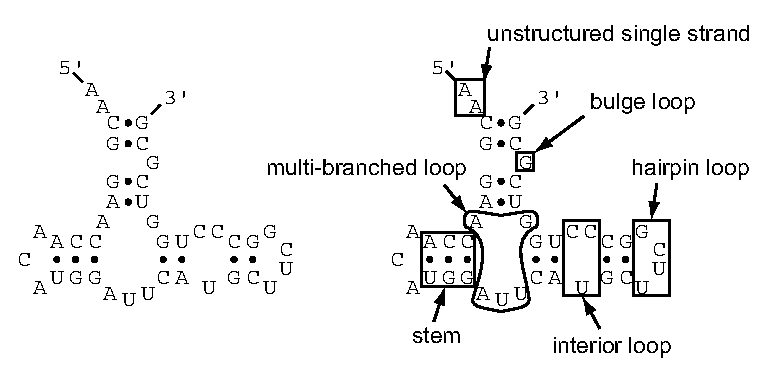
\includegraphics[scale=0.8]{Figures/rna_elements}
\end{center}
\begin{center}
\begin{BVerbatim}
  ::((((,<<<___>>>,,,<<-<<____>>-->>,))-))
  AACGGAACCAACAUGGAUUCAUGCUUCGGCCCUGGUCGCG
\end{BVerbatim}
\end{center}

\subsubsection{Full (output) WUSS notation}

In detail, symbols used by WUSS notation in \emph{output} structure
annotation strings are as follows:

\begin{sreitems}{\textbf{Bulge, interior loops}}
\item[\textbf{Base pairs}]
  Base pairs are annotated by nested matching pairs of symbols
  \verb+<>+, \verb+()+, \verb+[]+, or \verb+{}+.
  The different symbols indicate the ``depth'' of the
  helix in the RNA structure as follows:
  \verb+<>+ are used for simple terminal stems; 
  \verb+()+ are used for ``internal'' helices enclosing a multifurcation of
  all terminal stems; \verb+[]+ are used for internal helices 
  enclosing a multifurcation that includes at least one annotated
  \verb+()+ stem already; and \verb+{}+ are used for all internal
  helices enclosing deeper multifurcations.
   
\item[\textbf{Hairpin loops}]
  Hairpin loop residues are indicated by underscores, \verb+_+.
  Simple stem loops stand out as, e.g.\ \verb+<<<<____>>>>+.

\item[\textbf{Bulge, interior loops}]
  Bulge and interior loop residues are indicated by dashes, \verb+-+.
  
\item[\textbf{Multifurcation loops}]
  Multifurcation loop residues are indicated by commas, \verb+,+.
  The mnemonic is ``stem 1, stem2'', e.g.\ \verb+<<<___>>>,,<<<___>>>+.

\item[\textbf{External residues}]
  Unstructured single stranded residues completely outside the
  structure (unenclosed by any base pairs) are annotated by
  colons, \verb+:+.

\item[\textbf{Insertions}]
  Insertions relative to a known structure are indicated by periods,
  \verb+.+. Regions where local structural alignment was invoked,
  leaving regions of both target and query sequence unaligned,
  are indicated by tildes, \verb+~+. These symbols only appear in
  alignments of a known (query) structure annotation to a target
  sequence of unknown structure.

\item[\textbf{Pseudoknots}]
  WUSS notation allows pseudoknots to be annotated as pairs of
  upper case/lower case letters: for example,
  \verb+<<<<_AAAA____>>>>aaaa+ annotates a simple pseudoknot;
  additional pseudoknotted stems could be annotated by \verb+Bb+,
  \verb+Cc+, etc. Infernal cannot handle pseudoknots, however;
  pseudoknot notation never appears in Infernal output; it
  is accepted in input files, but ignored.
\end{sreitems}

An example of WUSS notation for a complicated structure
(\emph{E. coli} RNase P) is shown in Figure~\ref{fig:RNaseP}.  An
example of WUSS notation for a local Infernal alignment of
\emph{B. subtilis} RNase P to \emph{E. coli} RNase P, illustrating the
use of local alignment annotation symbols, is in
Figure~\ref{fig:bsu-alignment}.

\begin{figure}[tp]
\begin{center}
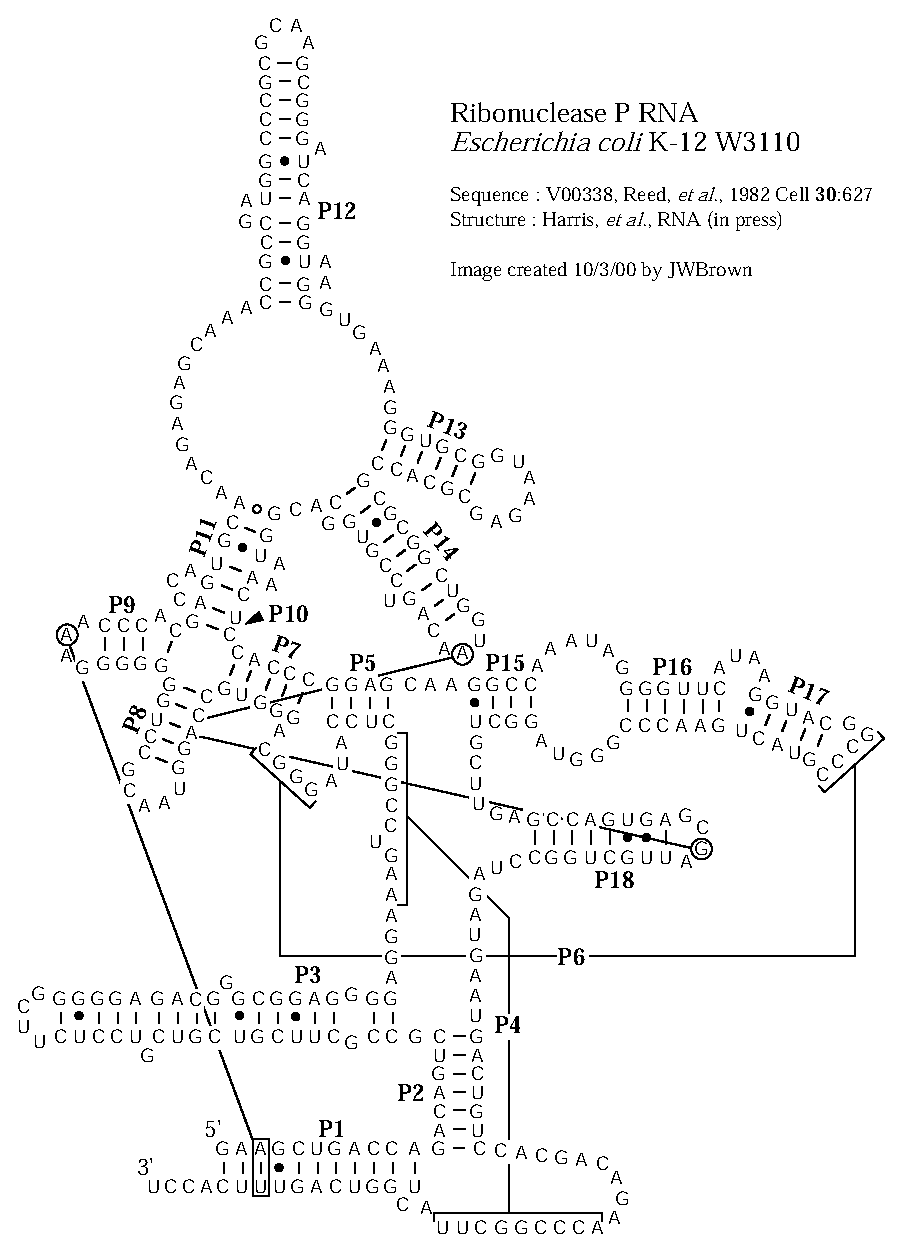
\includegraphics[scale=0.6]{Figures/rnaseP-ecoli}
\end{center}        
\begin{center}
{\scriptsize
\begin{BVerbatim}
           {{{{{{{{{{{{{{{{{{,<<<<<<<<<<<<<-<<<<<____>>>>>>>>>->>>>>>>>
         1 GAAGCUGACCAGACAGUCGCCGCUUCGUCGUCGUCCUCUUCGGGGGAGACGGGCGGAGGG 60      

           >,,,,,,,,,,,,,[[[[--------[[[[[<<<<<_____>>>>><<<<____>>>->(
        61 GAGGAAAGUCCGGGCUCCAUAGGGCAGGGUGCCAGGUAACGCCUGGGGGGGAAACCCACG 120     

           (---(((((,,,,,,,,,,,,<<<<<--<<<<<<<<____>>>>>->>>>>>-->>,,,,
       121 ACCAGUGCAACAGAGAGCAAACCGCCGAUGGCCCGCGCAAGCGGGAUCAGGUAAGGGUGA 180     

           ,,,<<<<<<_______>>>>>><<<<<<<<<____>>>->>>>>->,,)))--))))]]]
       181 AAGGGUGCGGUAAGAGCGCACCGCGCGGCUGGUAACAGUCCGUGGCACGGUAAACUCCAC 240     

           ]]]]]],,,<<<<------<<<<<<----<<<<<_____>>>>>>>>>>>----->>>>,
       241 CCGGAGCAAGGCCAAAUAGGGGUUCAUAAGGUACGGCCCGUACUGAACCCGGGUAGGCUG 300     

           ,,,,,<<<<<<<<____>>>>>>>>,,,,,,,,,,}}}}}}}------------------
       301 CUUGAGCCAGUGAGCGAUUGCUGGCCUAGAUGAAUGACUGUCCACGACAGAACCCGGCUU 360     

           -}-}}}}}}}}}}::::
       361 AUCGGUCAGUUUCACCU 377     
\end{BVerbatim} 
}
\end{center}
\caption{\small \textbf{Example of WUSS notation.} Top: Secondary
structure of \emph{E. coli} RNase P, from Jim Brown's RNase P database
\citep{Brown99}. Bottom: WUSS notation for the same structure,
annotating the \emph{E. coli} RNase P sequence. The P4 and P6
pseudoknots are not annotated in this example.}
\label{fig:RNaseP}
\end{figure}

\begin{figure}[tp]
\begin{center}
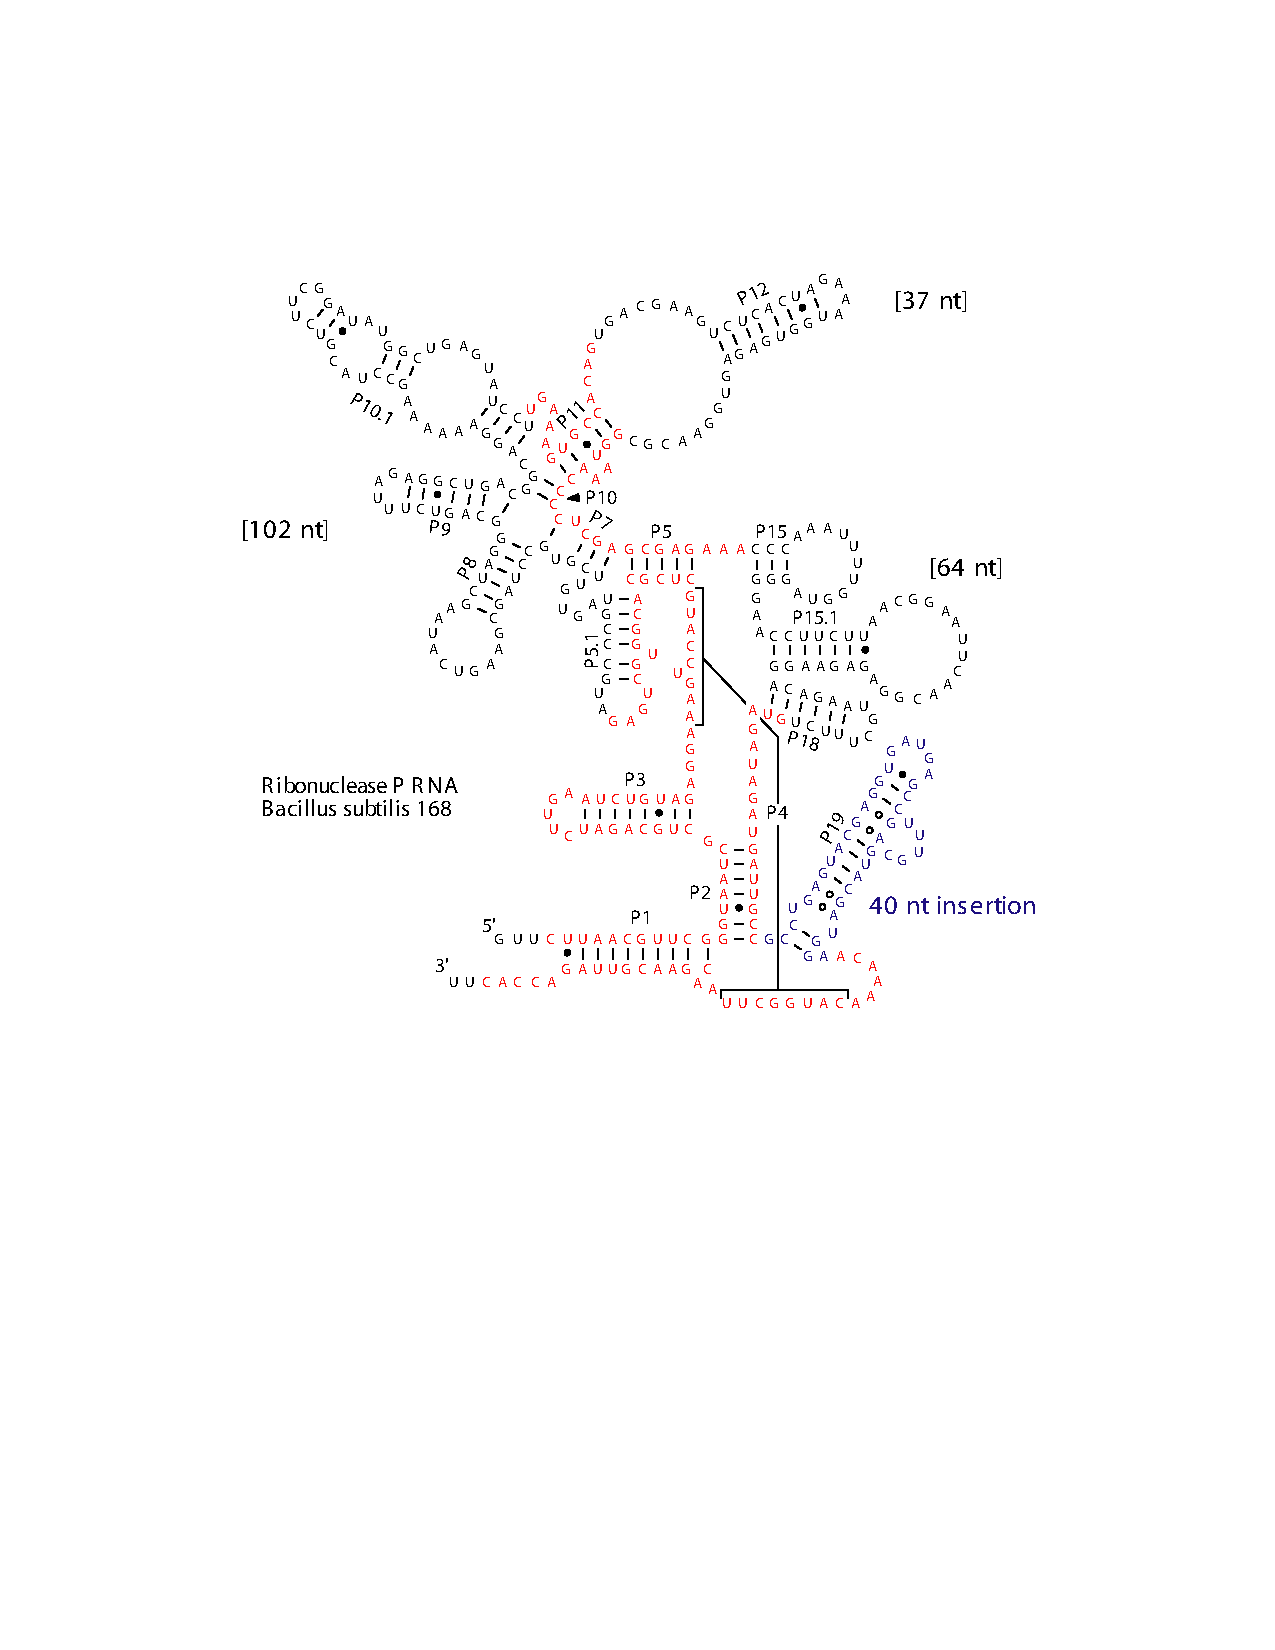
\includegraphics[scale=0.6]{Figures/rnaseP-bsu-alignment}
\end{center}
\begin{center}
{\scriptsize
\begin{BVerbatim}
>> M13175.1  
 rank     E-value  score  bias mdl mdl from   mdl to       seq from      seq to       acc trunc   gc
 ----   --------- ------ ----- --- -------- --------    ----------- -----------      ---- ----- ----
  (1) !   2.2e-20   58.0   0.0  cm        1      367 []           4         399 + .. 0.77    no 0.49

                    v                          v      v                                  vv         vvvvv    vvvv vv NC
                    {{{{{{{{{{{{{{{{{{,<<<<<<<<<______>>>>>>>>>,,,,,,,,,,,,,[[[[.--------[[[[[~~~~~~<<<<<____>>>>->( CS
  RNaseP_bact_a   1 cgagccggccgggcggucGCgcccccccuuaaaagggggggcGAGGAAAGUCCGGgCUcC.AcAGGgCAggguG*[15]*cggggGugAccccAgG 104
                       ::CG::CGGG:::UCGC::C:::: U      ::::G::GAGGAAAGUCC  GCUC  AC G GC   G:G               +++C + 
       M13175.1   4 CUUAACGUUCGGGUAAUCGCUGCAGAUCU---UGAAUCUGUAGAGGAAAGUCCAUGCUCGcACGGUGCU--GAG*[96]*---------UAUCCUU 175
                    **************************974...4579**********************98788777776..555...8...........3444468 PP

                                                                                           v   vv        vvvv        NC
                    (---(((((,,,,,,,,,,,,<<<<<<<<<<<____>>>>>>>>>-->>,,,,,,~~~~~~,,)))--))))]]]]].]]]],,,<<<<-----   CS
  RNaseP_bact_a 105 GAaAGugCcACAGAAAaaAgACCgCccgccccuuaaggggcggGcAAGGGUGAAA*[43]*uagGcAAaCCCCaccc.GgAGCAAggccAAAUA   234
                    GAAAGU:CCACAG +A  A+ :C   :::C:: +AA::G:::     G:GUG AA        GG:AAACC C:C +  GAG AA  C+AA U 
       M13175.1 176 GAAAGUGCCACAGUGACGAAGUC---UCACUAGAAAUGGUGA-----GAGUGGAA*[ 1]*GCGGUAAACCCCUCGAgCGAGAAACCCAAAUUU   256
                    99*****************8866...4455558888555444.....66999987...6..99********97665577899888765444332   PP

                          vvvv                                                                                       NC
                    ~~~~~~>>>>,,,,,,<<<<<<.<<____>>>>>>>>,,,,,,,,,,}}}}}}}---------------........................--- CS
  RNaseP_bact_a 235 *[39]*ggccGCUuGAGccggc.cgGuAAcggccggCCuAGAugAAUgaccgcccucuuguuaaauuuu........................aAC 338
                              G     :::: : C:G AA:G: :::: UAGAU++AUGA:::CC  CU + UA  +  U                        AAC
       M13175.1 257 *[32]*----GAG---AGAAGGaCAG-AAUGCUUUCUGUAGAUAGAUGAUUGCCGCCUGAGUACGAGGUgaugagccguuugcaguacgauggAAC 370
                    ...3......222...2222221222.335555566699****************9998888888888899999********************** PP

                                            v     NC
                    -------------}-}}}}}}}}}}:::: CS
  RNaseP_bact_a 339 AGAAcCCGGCUUAcaggccggcucgucuu 367
                    A AAC  GGCUUACAG::CG::    C+ 
       M13175.1 371 AAAACAUGGCUUACAGAACGUUAGACCAC 399
                    ***************************** PP
\end{BVerbatim}
}
\end{center}
\caption{\small \textbf{Local alignment annotation example.} Top:
Secondary structure of \emph{B. subtilis} RNase P, from Jim Brown's
RNase P database \citep{Brown99}. Residues in red are those that
Infernal aligns to a CM of \emph{E. coli} type RNase P's
(the RNase P bacterial type A model built from the Rfam 10.1 RF00010
seed alignment using default Infernal 1.1 \prog{cmbuild} and
\prog{cmcalibrate}). The local structural alignment is in four pieces;
three regions of the structure (96, 1, and 32 nt long) are skipped
over (i.e. not aligned to the type A model). One additional stem is
treated as a 24 nt insertion.  Bottom: the Infernal \prog{cmsearch}
output showing the RNase P type A query model, which corresponds
closely to the \emph{E. coli} structure, aligned to the
\emph{B. subtilis} sequence. The three skipped regions (96, 1, and 32
nt long) of the \emph{B. subtilis} structure from the top of the
figure are ``local end'' emissions which skip 15, 43, and 39 consensus
positions of the type A model, respectively.}
\label{fig:bsu-alignment}
\end{figure}

\subsubsection{Shorthand (input) WUSS notation}

While WUSS notation makes it easier to visually interpret
Infernal \emph{output} structural annotation, it would be
painful to be required to \emph{input} all structures in full WUSS
notation. Therefore when Infernal reads input secondary
structure annotation, it uses simpler rules:

\begin{sreitems}{\textbf{Single stranded residues}}
\item [\textbf{Base pairs}]
  Any matching nested pair of \verb+()+, \verb+()+, \verb+[]+, \verb+{}+
  symbols indicates a base pair; the exact choice of symbol has no
  meaning, so long as the left and right partners match up.

\item [\textbf{Single stranded residues}]
  All other symbols \verb+_-,:.~+ 
  indicate single stranded residues.
  The choice of symbol has no special meaning.
  Annotated pseudoknots (nested matched pairs of upper/lower case
  alphabetic characters) are also interpreted as single
  stranded residue in Infernal input.
\end{sreitems}

Thus, for instance, \verb+<<<<....>>>>+ and \verb+((((____))))+ and
\verb+<(<(._._)>)>+ all indicate a four base stem with a four base
loop (the last example is legal but weird). 

Remember that the key property of canonical (nonpseudoknotted) RNA
secondary structure is that the pairs are \emph{nested}.
\verb+((<<....))>>+ is not a legal annotation string: the pair symbols
don't match up properly. Infernal will reject such an
annotation and report an input format error, suspecting a problem with
your annotation.  If you want to annotate pseudoknots, WUSS notation
allows alphabetic symbols Aa, Bb, etc.\, see above; but remember that
Infernal ignores pseudoknotted stems and treats them as
single stranded residues.

Because many other RNA secondary structure analysis programs use a
simple bracket notation for annotating structure,
Infernal's ability to input this format makes it easier to
use data generated by other RNA software packages. Conversely,
converting Infernal output WUSS notation to simple bracket
notation is a matter of a simple Perl or sed script, substituting the
symbols appropriately.

\subsection{Stockholm, the recommended multiple sequence alignment format}

The Rfam and Pfam Consortiums have developed a multiple sequence
alignment format called ``Stockholm format'' that allows rich and
extensible annotation. 

Crucially for Infernal, Stockholm alignments support the annotation of 
a consensus secondary structure, which is why \prog{cmbuild} requires
its input alignment files to be in Stockholm format. Here is a minimal
Stockholm file with consensus secondary structure annotation in
shorthand WUSS notation (described earlier in this section).

\begin{sreoutput}
# STOCKHOLM 1.0

seq1           ACCGUC...GCAA...GG
seq2           ACCGUC...GCAA...GG
seq3           .CCUUCGUCGGAUGACGA
#=GC SS_cons   ...<<<..........>>

seq1           CGAUAC
seq2           CG..AC
seq3           ACAUCC
#=GC SS_cons   >.....
//
\end{sreoutput}

The first line in the file must be \verb+# STOCKHOLM 1.x+, where
\verb+x+ is a minor version number for the format specification
(and which currently has no effect on my parsers). This line allows a
parser to instantly identify the file format.

In the alignment, each line contains a name, followed by the aligned
sequence. A dash, period, underscore, or tilde (but not whitespace)
denotes a gap. If the alignment is too long to fit on one line, the
alignment may be split into multiple blocks, with blocks separated by
blank lines, as this example is. The number of sequences, their order,
and their names must be the same in every block. Within a given block,
each (sub)sequence (and any associated \verb+#=GR+ and \verb+#=GC+
markup, such as the \verb+SS_cons+ lines, see below) is of equal
length, called the \textit{block length}. Block lengths may differ
from block to block. The block length must be at least one residue,
and there is no maximum. 

Other blank lines are ignored. You can add comments anywhere to the
file (even within a block) on lines starting with a \verb+#+.

The \verb+SS_cons+ line defines the consensus secondary structure in
shorthand WUSS notation, as described earlier in 
this section.

All other annotation is added using a tag/value comment style. The
tag/value format is inherently extensible, and readily made
backwards-compatible; unrecognized tags will simply be ignored. Extra
annotation includes individual sequence RNA or protein secondary
structure, sequence weights, a reference coordinate system for the
columns, and database source information including name, accession
number, and coordinates (for subsequences extracted from a longer
source sequence) See below for details.

\subsubsection{syntax of Stockholm markup}

There are four types of Stockholm markup annotation, for per-file,
per-sequence, per-column, and per-residue annotation:

\begin{sreitems}{\emprog{\#=GR <seqname> <tag> <..s..>}}
\item [\emprog{\#=GF <tag> <s>}]
        Per-file annotation. \prog{<s>} is a free format text line
        of annotation type \prog{<tag>}. For example, \prog{\#=GF DATE
        April 1, 2000}. Can occur anywhere in the file, but usually
        all the \prog{\#=GF} markups occur in a header.

\item [\emprog{\#=GS <seqname> <tag> <s>}]
        Per-sequence annotation. \prog{<s>} is a free format text line
        of annotation type \prog{tag} associated with the sequence
        named \prog{<seqname>}. For example, \prog{\#=GS seq1
        SPECIES\_SOURCE Caenorhabditis elegans}. Can occur anywhere
        in the file, but in single-block formats (e.g. the Pfam
        distribution) will typically follow on the line after the
        sequence itself, and in multi-block formats (e.g. Infernal
        output), will typically occur in the header preceding the
        alignment but following the \prog{\#=GF} annotation.

\item [\emprog{\#=GC <tag> <..s..>}]
        Per-column annotation. \prog{<..s..>} is an aligned text line
        of annotation type \prog{<tag>}.
        \verb+#=GC+ lines are
        associated with a sequence alignment block; \prog{<..s..>}
        is aligned to the residues in the alignment block, and has
        the same length as the rest of the block.
        Typically \verb+#=GC+ lines are placed at the end of each block.

\item [\emprog{\#=GR <seqname> <tag> <..s..>}]
        Per-residue annotation. \prog{<..s..>} is an aligned text line
        of annotation type \prog{<tag>}, associated with the sequence
        named \prog{<seqname>}. 
        \verb+#=GR+ lines are 
        associated with one sequence in a sequence alignment block; 
        \prog{<..s..>}
        is aligned to the residues in that sequence, and has
        the same length as the rest of the block.
        Typically
        \verb+#=GR+ lines are placed immediately following the
        aligned sequence they annotate.
\end{sreitems}

\subsubsection{semantics of Stockholm markup}

Any Stockholm parser will accept syntactically correct files, but is
not obligated to do anything with the markup lines. It is up to the
application whether it will attempt to interpret the meaning (the
semantics) of the markup in a useful way. At the two extremes are the
Belvu alignment viewer and the Infernal and HMMER 
software packages.

Belvu simply reads Stockholm markup and displays it, without trying to
interpret it at all. The tag types (\prog{\#=GF}, etc.) are sufficient
to tell Belvu how to display the markup: whether it is attached to the
whole file, sequences, columns, or residues.

Infernal uses Stockholm markup to pick up a variety of information
from the Rfam multiple alignment database. The Rfam consortium
therefore agrees on additional syntax for certain tag types, so
Infernal can parse some markups for useful information. This
additional syntax is imposed by Rfam, Pfam, Infernal, HMMER, and other
software from our lab, not by Stockholm format per se. You can think
of Stockholm as akin to XML, and what our software reads as akin
to an XML DTD, if you're into that sort of structured data format
lingo.

The Stockholm markup tags that are parsed semantically by Infernal
are as follows:

\subsubsection{recognized \#=GF annotations}
\begin{sreitems}{\emprog{TC  <f> <f>}}
\item [\emprog{ID  <s>}] 
        Identifier. \emprog{<s>} is a name for the alignment;
        e.g. ``RNaseP''. One word. Unique in file.

\item [\emprog{AC  <s>}]
        Accession. \emprog{<s>} is a unique accession number for the
        alignment; e.g. 
        ``RF00001''. Used by the Rfam database, for instance. 
        Often a alphabetical prefix indicating the database
        (e.g. ``RF'') followed by a unique numerical accession.
        One word. Unique in file. 
        
\item [\emprog{DE  <s>}]
        Description. \emprog{<s>} is a free format line giving
        a description of the alignment; e.g.
        ``Ribonuclease P RNA''. One line. Unique in file.

\item [\emprog{AU  <s>}]
        Author. \emprog{<s>} is a free format line listing the 
        authors responsible for an alignment; e.g. 
        ``Bateman A''. One line. Unique in file.

\item [\emprog{GA  <f>}]
        Gathering threshold. The Infernal bit score cutoff 
        used in gathering the members of Rfam full alignments. 
        
\item [\emprog{NC <f>}] 
        Noise cutoff. The Infernal bit score cutoff, set according to
        the highest scores seen for nonhomologous sequence hits when
        gathering members of Rfam full alignments.

\item [\emprog{TC  <f>}]
        Trusted cutoff. The Infernal bit score cutoff, set according
        to the lowest scores seen for true homologous sequence hits
        that were above the GA gathering thresholds, when gathering
        members of Rfam full alignments.
\end{sreitems}

\subsubsection{recognized \#=GS annotations}

\begin{sreitems}{\emprog{WT  <f>}}
\item [\emprog{WT  <f>}]
        Weight. \emprog{<f>} is a positive real number giving the
        relative weight for a sequence, usually used to compensate
        for biased representation by downweighting similar sequences.   
        Usually the weights average 1.0 (e.g. the weights sum to
        the number of sequences in the alignment) but this is not
        required. Either every sequence must have a weight annotated, 
        or none of them can.  

\item [\emprog{AC  <s>}]
        Accession. \emprog{<s>} is a database accession number for 
        this sequence. (Compare the \prog{\#=GF AC} markup, which gives
        an accession for the whole alignment.) One word. 
        
\item [\emprog{DE  <s>}]
        Description. \emprog{<s>} is one line giving a description for
        this sequence. (Compare the \prog{\#=GF DE} markup, which gives
        a description for the whole alignment.)
\end{sreitems}


\subsubsection{recognized \#=GC annotations}

\begin{sreitems}{\emprog{SS\_cons}}
\item [\emprog{RF}]
        Reference line. Any character is accepted as a markup for a
        column. The intent is to allow labeling the columns with some
        sort of mark. \prog{cmbuild} uses this annotation to determine
        which columns are consensus versus insertion if the
        \prog{--hand} option is used; insertion columns are annotated
        by a gap symbol, and consensus columns by any non-gap symbol.
        
\item [\emprog{SS\_cons}]
	Secondary structure consensus.  When this line is generated by
        Infernal, it is generated in full WUSS notation.
        When it is read by \prog{cmbuild}, it is interpreted more
        loosely, in shorthand (input) WUSS notation: pairs of symbols
        \verb+<>+, \verb+()+, \verb+[]+, or \verb+[]+ mark consensus
        base pairs, and symbols \verb+:_-,.~+ mark single stranded
        columns (see the section on WUSS format above for details).

\end{sreitems}

\subsubsection{recognized \#=GR annotations}
\begin{sreitems}{\emprog{SS}}
\item [\emprog{SS}]
        Secondary structure consensus. See \prog{\#=GC SS\_cons}
        above.

\item [\emprog{PP}] Posterior probability for an aligned residue. This
  represents the probability that this residue is assigned to the CM
  state corresponding to this alignment column, as opposed to some
  other state. The posterior
  probability is encoded as 11 possible characters \verb+0-9*+: $0.0
  \leq p < 0.05$ is coded as 0, $0.05 \leq p < 0.15$ is coded as 1,
  (... and so on ...), $0.85 \leq p < 0.95$ is coded as 9, and $0.95
  \leq p \leq 1.0$ is coded as '*'. Gap characters appear in the PP
  line where no residue has been assigned.
\end{sreitems}

\subsection{Sequence files: FASTA format}

FASTA is probably the simplest of formats for unaligned sequences.
FASTA files are easily created in a text editor.  Each sequence is
preceded by a line starting with \verb+>+. The first word on this line
is the name of the sequence. The rest of the line is a description of
the sequence (free format). The remaining lines contain the sequence
itself. You can put as many letters on a sequence line as you want.
For example:

\begin{sreoutput}
>seq1 This is the description of my first sequence.
AGTACGTAGTAGCTGCTGCTACGTGCGCTAGCTAGTACGTCA CGACGTAGATGCTAGCTGACTCGATGC
>seq2 This is a description of my second sequence.
CGATCGATCGTACGTCGACTGATCGTAGCTACGTCGTACGTAG CATCGTCAGTTACTGCATGCTCG
CATCAGGCATGCTGCTGACTGATCGTACG
\end{sreoutput}

For better or worse, FASTA is not a documented standard. Minor (and
major) variants are in widespread use in the bioinformatics community,
all of which are called ``FASTA format''. My software attempts to
cater to all of them, and is tolerant of common deviations in FASTA
format. Certainly anything that is accepted by the database formatting
programs in NCBI BLAST or WU-BLAST (e.g. setdb, pressdb, xdformat)
will also be accepted by my software. Blank lines in a FASTA file are
ignored, and so are spaces or other gap symbols (dashes, underscores,
periods) in a sequence. Other non-amino or non-nucleic acid symbols in
the sequence are also silently ignored, mostly because some people
seem to think that ``*'' or ``.'' should be added to protein sequences
to (redundantly) indicate the end of the sequence. The parser will
also accept unlimited line lengths, which allows it to accomodate the
enormous description lines in the NCBI NR databases.

(On the other hand, any FASTA files \emph{generated} by my software
adhere closely to community standards, and should be usable by other
software packages (BLAST, FASTA, etc.) that are more picky about
parsing their input files. That means you can run a sloppy FASTA file
thru the \prog{sreformat} utility program to clean it up.)

Partly because of this tolerance, the software may have a difficult
time dealing with files that are \textit{not} in FASTA format,
especially if you're relying on file format autodetection (the
``Babelfish'').  Some (now mercifully uncommon) file formats are so
similar to FASTA format that they be erroneously called FASTA by the
Babelfish and then quietly and lethally misparsed. An example is the
old NBRF file format. If you're afraid of this, you can use the
\prog{--informat fasta} option to bypass the Babelfish and improve
robustness. However, it is still possible to construct files
perversely similar to FASTA that will still confuse the parser.  (The
gist of these caveats applies to all formats, not just FASTA.)

\subsection{Null model file format}

The Infernal source distribution includes an example null model file, 
\prog{src/rna.null}. This null model is identical to the hardcoded default
prior used by Infernal, all four RNA nucleotides are equiprobable in
the null, background model. 

A null model file must contain exactly four non-comment lines. A
comment line begins with a ``\# ``, that is a \# followed by a single
space. Each of the four non-comment lines must contain a single floating point
number, the four of which sum to 1.0. The first non-comment line is interpreted as
the background probability of an ``A'' residue, the second, third, and
fourth non-comment lines are interpreted as the background
probabilities of a ``C'', ``G'' and ``U'' respectively. 

\subsection{Clan input file format for cmscan}

The \ccode{cmscan} program has a \ccode{--clanin <f>} option that
allows the user to supply an input file \ccode{<f>} with information
on clan membership for models in the CM file. This option must be used
in combination with the \ccode{--tblout} and \ccode{--fmt 2}
options. An example clan input file is included with the Infernal
source distribution, \ccode{tutorial/Rfam.12.1.clanin}. This file
specifies the clan membership for the 2474 models in the Rfam 12.1
release, of which 311 models belong to 104 clans. This file should be
used in combination with the Rfam.cm file for Rfam 12.1, available for
download as a gzipped file here:
\url{ftp://ftp.ebi.ac.uk/pub/databases/Rfam/12.1/Rfam.cm.gz}. Note that
many of the Rfam models are not members of a clan; the clan input file does
not need to specify clan membership for all models in the CM file.

A clan input file contains one line per clan. Each line must contain
at least two space-delimited tokens. The first token is the name of
the clan (this name cannot contain spaces). Each token after the first
is the name of a model that is a member of the clan named in the first
token. These tokens must be valid names of models in the file CM file
you are using with \ccode{cmscan}. These tokens cannot be the
accessions of models. Valid model names cannot contain spaces
(enforced by \prog{cmbuild} during model construction). To determine
the names of models in a CM file, use \ccode{cmstat}. 

For example, in the file \ccode{tutorial/Rfam.12.1.clanin} the first token
of the first line is ``CL00001'' and tokens two through five are
``tRNA'', ``cyano\_tmRNA'', ``tRNA-Sec'', ``mt-tmRNA'', indicating
that these four models are members of the CL00001 clan. \ccode{cmscan}
will output the clan name of models in clans in its tabular output
file specified with \ccode{--tblout} when the \ccode{--fmt 2} option
is also used. Furthermore, you can specify
that only overlapping hits between models of the same clan are
annotated (as opposed to all overlapping hits) in the tabular output
file by additionally using the \ccode{--oclan} option. Finally, you
can specify that lower scoring overlaps within clans are not output by
additionally using the \ccode{--oskip} and the \ccode{--oclan}
options.





\subsection{Dirichlet prior files}
% Documentation of Infernal's Dirichlet prior file format
%
% Uses no sectioning commands, so it may be included as a subsection of
% a section, or a section in a chapter of file formats.
% The .tex file that includes this one provides the \section{} header.
%  
% SRE, Wed Apr  6 13:46:43 2005

A prior file is parsed into a number of whitespace-delimited,
non-comment fields. These fields are then interpreted in order.  The
order and number of the fields is important. This is not a robust,
tag-value save file format.

All whitespace is ignored, including newlines. The number of fields
per line is unimportant.

Comments begin with a \verb+#+ character. The remainder of any line
following a \verb+#+ is ignored.

The Infernal source distribution includes an example prior file,
\prog{default.pri}. This prior is identical to the hardcoded default
prior used by Infernal. The following text may only make sense if
you're looking at that example while you read.

The order of the fields in the prior file is as follows:

\begin{description}
\item[\textbf{Strategy.}] The first field is the keyword
  \emprog{Dirichlet}. Currently Dirichlet priors (mixture or not)
  are the only prior strategy used by Infernal.

\item[\textbf{Transition prior section.}] The next field is the number
  \emprog{74}, the number of different types of transition
  distributions. (See Figure~\ref{fig:magic74} for an explanation of
  where the number 74 comes from.) Then, for each of these 74
  distributions:

  \begin{description}
  \item{\emprog{<from-uniqstate> <to-node>}:} Two fields give the
  transition type: from a unique state identifier, to a node
  identifier. Example: \emprog{MATP\_MP MATP}. 

  \item{\emprog{<n>}:} One field gives the number of transition
  probabilities for this transition type; that is, the number of
  Dirichlet parameter vector $\alpha^q_1..\alpha^q_n$ for each mixture
  component $q$.

  \item{\emprog{<nq>}:} One field gives the number of mixture
  Dirichlet components for this transition type's prior. Then,
  for each of these \emprog{nq} Dirichlet components:

     \begin{description}
     \item{\emprog{p(q)}:} One field gives the mixture coefficient $p(q)$,
     the prior probability of this component $q$. For a single-component
     ``mixture'', this is always 1.0.

     \item{$\mathbf{\alpha^q_1..\alpha^q_n}$:} The next $n$ fields give the
     Dirichlet parameter vector for this mixture component $q$.
     \end{description}
  \end{description}

\item[\textbf{Base pair emission prior section.}] This next section is
  the prior for MATP\_MP emissions. One field gives \emprog{<K>}, the
  ``alphabet size'' -- the number of base pair emission probabilities
  -- which is always 16 (4x4), for RNA. The next field gives \emprog{<nq>}, the
  number of mixture components. Then, for each of these \emprog{nq}
  Dirichlet components:
     \begin{description}
     \item{\emprog{p(q)}:} One field gives the mixture coefficient $p(q)$,
     the prior probability of this component $q$. For a single-component
     ``mixture'', this is always 1.0.

     \item{$\mathbf{\alpha^q_{AA}..\alpha^q_{UU}}$:} The next 16 fields give the
     Dirichlet parameter vector for this mixture component, in alphabetical
     order (AA, AC, AG, AU, CA \ldots GU, UA, UC, UG, UU). 
     \end{description}

\item[\textbf{Consensus singlet base emission prior section.}] This
  next section is the prior for MATL\_ML and MATR\_MR emissions.  One
  field gives \emprog{<K>}, the ``alphabet size'' -- the number of
  singlet emission probabilities -- which is always 4, for RNA.  The
  next field gives \emprog{<nq>}, the number of mixture components. Then,
  for each of these \emprog{nq} Dirichlet components:
     \begin{description}
     \item{\emprog{p(q)}:} One field gives the mixture coefficient $p(q)$,
     the prior probability of this component $q$. For a single-component
     ``mixture'', this is always 1.0.

     \item{$\mathbf{\alpha^q_A..\alpha^q_U}$:} The next 4 fields give the
     Dirichlet parameter vector for this mixture component, in alphabetical
     order (A, C, G, U).
     \end{description}
  
\item[\textbf{Nonconsensus singlet base emission prior section.}] This
  next section is the prior for insertions (MATP\_IL, MATP\_IR,
  MATL\_IL, MATR\_IR, ROOT\_IL, ROOT\_IR, BEGR\_IL) as well as
  nonconsensus singlets (MATP\_ML, MATP\_MR). 
  One field gives \emprog{<K>}, the ``alphabet size'' -- the number of
  singlet emission probabilities -- which is always 4, for RNA. 
  The next field gives \emprog{<nq>}, the
  number of mixture components. Then, for each of these \emprog{nq}
  Dirichlet components:
     \begin{description}
     \item{\emprog{p(q)}:} One field gives the mixture coefficient $p(q)$,
     the prior probability of this component $q$. For a single-component
     ``mixture'', this is always 1.0.

     \item{$\mathbf{\alpha^q_A..\alpha^q_U}$:} The next 4 fields give the
     Dirichlet parameter vector for this mixture component, in alphabetical
     order (A, C, G, U).
     \end{description}
\end{description}


\begin{figure}[htp]
\begin{center}
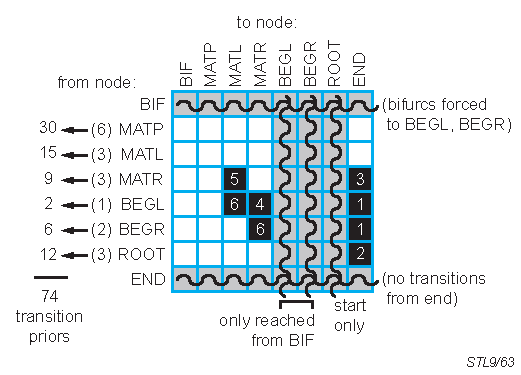
\includegraphics{Figures/stl9-63}
\end{center}
\caption{\small\textbf{Where does the magic number of 74 transition
distribution types come from?} The transition distributions are
indexed in a 2D array, from a unique statetype (20 possible) to a
downstream node (8 possible), so the total conceivable number of
different distributions is $20 \times 8 = 160$. The grid represents
these possibilities by showing the $8 \times 8$ array of all node
types to all node types; each starting node contains 1 or more unique
states (number in parentheses to the left).
Two rows are impossible (gray): bifurcations automatically transit to
determined BEGL, BEGR states with probability 1, and end nodes have no
transitions.  Three columns are impossible (gray): BEGL and BEGR can
only be reached by probability 1 transitions from a bifurcation, and
the ROOT node is special and can only start a model. 
Eight individual cells of the grid are unused (black) because of the
way \prog{cmbuild} (almost) unambiguously constructs a guide tree from
a consensus structure.  These cases are numbered as follows. (1) BEGL
and BEGR never transit to END; this would imply an empty
substructure. A bifurcation is only used if both sides of the split
contain at least one consensus pair (MATP). (2) ROOT never transits to
END; this would imply an alignment with zero consensus
columns. Infernal models assume $\geq 1$ consensus columns. (3) MATR
never transits to END. Infernal always uses MATL for unpaired columns
whenever possible. MATR is only used for internal loops,
multifurcation loops, and 3' bulges, so MATR must always be followed
by a BIF, MATP, or another MATR. (4) BEGL never transits to MATR. The
single stranded region between two bifurcated stems is unambiguously
assigned to MATL nodes on the right side of the split, not to MATR
nodes on the left. (5) MATR never transits to MATL. The only place
where this could arise (given that we already specified that MATL is
used whenever possible) is in an interior loop; there, by unambiguous
convention, MATL nodes precede MATR nodes. (6) BEGL nodes never
transit to MATL, and BEGR nodes never transit to MATR. By convention,
at any bifurcated subsequence $i,j$, $i$ and $j$ are paired but not to
each other. That is, the smallest possible subsequence is bifurcated,
so that any single stranded stretches to the left and right are
assigned to MATL and MATR nodes above the bifurcation, instead of MATL
nodes below the BEGL and MATR nodes below the BEGR.
Thus, the total number 74 comes from multiplying, for each row, the
number of unique states in each starting node by the number of
possible downstream nodes (white), and summing these up, as shown to
the left of the grid.}
\label{fig:magic74}
\end{figure}


\newpage
\section{Acknowledgements}

Infernal relies heavily on HMMER and Easel, originally created by Sean
Eddy. Several others have helped develop these two packages as well,
including Steve Johnson, Alex Coventry, Dawn Brooks, Sergi Castellano,
Michael Farrar, Travis Wheeler, and Elena Rivas.  In particular, the
improved speed of Infernal 1.1 is enabled by research and development
for the HMMER3 project, mainly from Sean, Travis and Michael. Further,
many of the changes made for Infernal 1.1 mirror features in HMMER3,
and were implemented frequently by stealing and slightly modifying
code. Even this guide is based heavily on HMMER3's guide, and some
analogous sections are identical or near identical.  Additionally, the
RSEARCH program \citep{KleinEddy03} from Robbie Klein has also had an
important impact on Infernal, which still includes some of its code.

Sean created and was the lone developer of Infernal up through the
version 0.55 release in 2003. Two graduate students, Diana Kolbe and
Eric Nawrocki, focused on improvements to Infernal for their graduate
work, beginning in 2004. Their efforts combined with Sean's led to
versions 0.56 through 1.0.2. Diana has moved onto a postdoc, but
included a snapshot of the codebase in between the 1.0.2 and 1.1
releases as supplementary material with her thesis. Eric continues to
develop Infernal and is responsible for most of the changes in the 1.1
release.

The concept of HMM banded SCFG alignment implemented in Infernal
derives from Michael Brown's RNACAD software, developed while he was
working with David Haussler at UC Santa Cruz \citep{Brown00}. HMM
filtering for CMs was pioneered by Zasha Weinberg and Larry Ruzzo at
the University of Washington
\citep{WeinbergRuzzo04,WeinbergRuzzo04b,WeinbergRuzzo06}. The CP9 HMMs
in Infernal are a reimplementation of a profile HMM architecture
introduced by Weinberg.

Infernal testing requires \emph{a lot} of compute power, and we are
extremely fortunate to have access to a highly reliable and
state-of-the-art computing cluster, thanks to Goran Ceric, Rob Lines,
Peter Bukowinski, Ken Carlile, Patrick Yeboah, and others here at
Janelia.

Infernal is primarily developed on GNU/Linux and Apple Macintosh
machines, but is tested on a variety of hardware. Over the years,
Compaq, IBM, Intel, Sun Microsystems, Silicon Graphics,
Hewlett-Packard, Paracel, and nVidia have provided generous hardware
support that makes this possible. We owe a large debt to the free
software community for the development tools we use: an incomplete
list includes GNU gcc, gdb, emacs, and autoconf; the amazing valgrind;
the indispensable Subversion; the ineffable perl; LaTeX and TeX;
PolyglotMan; and the UNIX and Linux operating systems.

\label{manualend}


\newpage
\bibliography{master,lab,books,local}
\end{document}
